% =============================================================
%  ΔΙΠΛΩΜΑΤΙΚΗ ΕΡΓΑΣΙΑ
%  Πανεπιστήμιο Αιγαίου - Πολυτεχνική Σχολή
%  Τμήμα Μηχανικών Πληροφοριακών και Επικοινωνιακών Συστημάτων
%
%  Compile with XeLaTeX (required for polyglossia/fontspec Greek support):
%     xelatex main.tex
%     biber main
%     xelatex main.tex
%     xelatex main.tex
%
%  On Overleaf: set the compiler to XeLaTeX (Menu -> Compiler -> XeLaTeX).
% =============================================================
\documentclass[12pt,a4paper,oneside]{book}

% ---------- Γλώσσα και γραμματοσειρά ----------
\usepackage{fontspec}
\usepackage{polyglossia}
\setmainlanguage{greek}
\setotherlanguage{english}

% TeX Gyre Termes: Times-συμβατή γραμματοσειρά με πλήρη κάλυψη ελληνικών
% γλυφών, διαθέσιμη by default στο Overleaf/TeX Live. Αν συντάσσετε τοπικά
% και θέλετε να χρησιμοποιήσετε την ίδια γραμματοσειρά με το πρότυπο .doc
% (Times New Roman), αντικαταστήστε τα δύο ονόματα παρακάτω με
% "Times New Roman".
\setmainfont{Times New Roman}
\newfontfamily\greekfont{Times New Roman}
% Μονόχωρη γραμματοσειρά για τα listings κώδικα του Παραρτήματος (τα
% σχόλια στον κώδικα είναι ούτως ή άλλως σε λατινικούς χαρακτήρες/greeklish
% για μέγιστη συμβατότητα).
\setmonofont{Consolas}

% ---------- Σελίδα / περιθώρια (όπως στο πρότυπο .doc: A4, ~2/2.25/2.5cm) ----------
\usepackage[a4paper,left=2cm,right=2.25cm,top=2.5cm,bottom=2.5cm]{geometry}
\usepackage{setspace}
\onehalfspacing

% ---------- Λοιπά πακέτα ----------
\usepackage{graphicx}
\usepackage{booktabs}
\usepackage{longtable}
\usepackage{array}
\usepackage{amsmath,amssymb}
\DeclareMathOperator*{\argmax}{arg\,max}
\usepackage{caption}
\usepackage{subcaption}
\usepackage{xcolor}
\usepackage{listings}
\usepackage{fancyhdr}
\usepackage{titlesec}
\usepackage[hidelinks]{hyperref}
\usepackage[backend=biber,style=ieee,sorting=none]{biblatex}
\addbibresource{references.bib}

% ---------- Ονόματα λιστών/ενοτήτων ώστε να ταιριάζουν ακριβώς με το πρότυπο ----------
\renewcommand{\contentsname}{Πίνακας περιεχομένων}
\renewcommand{\listfigurename}{Λίστα Σχημάτων}
\renewcommand{\listtablename}{Λίστα Πινάκων}
\renewcommand{\bibname}{Βιβλιογραφία}

% ---------- Κεφαλίδες ----------
\pagestyle{fancy}
\fancyhf{}
\fancyhead[R]{\small\thepage}
\fancyhead[L]{\small\leftmark}
\renewcommand{\headrulewidth}{0.4pt}
\setlength{\headheight}{14pt}

% ---------- Ρυθμίσεις listings για τμήματα κώδικα (MATLAB / Python) ----------
\lstdefinestyle{code}{
  basicstyle=\ttfamily\footnotesize,
  numbers=left,
  numberstyle=\tiny\color{gray},
  keywordstyle=\color{blue!70!black}\bfseries,
  commentstyle=\color{green!40!black}\itshape,
  stringstyle=\color{orange!70!black},
  breaklines=true,
  breakatwhitespace=false,
  frame=single,
  tabsize=2,
  columns=flexible,
  showstringspaces=false
}
\lstset{style=code}

\graphicspath{{figures/}}

\begin{document}

% ================= ΕΞΩΦΥΛΛΟ / ΠΡΟΛΟΓΙΚΕΣ ΣΕΛΙΔΕΣ =================
\frontmatter
\pagenumbering{gobble}

% Εξώφυλλο - προσαρμόστε [ΤΙΤΛΟΣ], επιβλέποντα και μέλη επιτροπής όταν οριστικοποιηθούν.
\begin{titlepage}
\centering
\vspace*{0.5cm}

{\large ΠΑΝΕΠΙΣΤΗΜΙΟ ΑΙΓΑΙΟΥ}\\[0.2cm]
{\large ΠΟΛΥΤΕΧΝΙΚΗ ΣΧΟΛΗ}\\[0.2cm]
{\large ΤΜΗΜΑ ΜΗΧΑΝΙΚΩΝ ΠΛΗΡΟΦΟΡΙΑΚΩΝ ΚΑΙ ΕΠΙΚΟΙΝΩΝΙΑΚΩΝ ΣΥΣΤΗΜΑΤΩΝ}\\[2.5cm]

\rule{0.8\textwidth}{0.4pt}\\[0.5cm]
{\large\itshape Multi-Connectivity Management in Integrated\\
Satellite-Terrestrial 6G Networks using Machine Learning Techniques}\\[0.5cm]
\rule{0.8\textwidth}{0.4pt}\\[0.2cm]

{\large ΔΙΠΛΩΜΑΤΙΚΗ ΕΡΓΑΣΙΑ}\\[0.3cm]
{\large του/της}\\[0.3cm]
{\large\bfseries Γεωργίου Ζάχου}\\[2.5cm]

\begin{flushleft}
\hspace{2cm}\begin{minipage}{0.7\textwidth}
\large
Επιβλέπων: \underline{\hspace{7cm}}\\[0.8cm]
Μέλη εξεταστικής επιτροπής:\\
\underline{\hspace{7cm}}\\[0.3cm]
\underline{\hspace{7cm}}
\end{minipage}
\end{flushleft}

\vfill
{\large Σάμος, \underline{\hspace{4cm}}}

\end{titlepage}

% Σκόπιμα λευκή σελίδα (όπως στο πρότυπο .doc)
\newpage
\thispagestyle{empty}
\vspace*{\fill}
\begin{center}
\itshape Η σελίδα αυτή είναι σκόπιμα λευκή.
\end{center}
\vspace*{\fill}
\newpage

\chapter*{Πρόλογος και ευχαριστίες}
\addcontentsline{toc}{chapter}{Πρόλογος και ευχαριστίες}

% TODO (προσωπικό κείμενο - συμπληρώστε πριν την κατάθεση):
% - Ευχαριστίες προς τον επιβλέποντα καθηγητή για την καθοδήγηση.
% - Ευχαριστίες προς οικογένεια/φίλους, αν επιθυμείτε.
% - Μία-δύο σύντομες παράγραφοι αρκούν, όπως αναφέρει και το πρότυπο.

Η παρούσα διπλωματική εργασία εκπονήθηκε στο Τμήμα Μηχανικών Πληροφοριακών
και Επικοινωνιακών Συστημάτων του Πανεπιστημίου Αιγαίου, στο πλαίσιο του
προπτυχιακού προγράμματος σπουδών.

Θα ήθελα να ευχαριστήσω τον επιβλέποντα καθηγητή μου για την καθοδήγηση,
τις εύστοχες παρατηρήσεις και την εμπιστοσύνη καθ' όλη τη διάρκεια
εκπόνησης της εργασίας.

\textit{[Συμπληρώστε εδώ τυχόν επιπλέον ευχαριστίες.]}

\newpage
\thispagestyle{empty}
\vspace*{\fill}
\begin{center}
\copyright\ 2026\\
του/της\\
\textbf{Γεωργίου Ζάχου}\\[0.5cm]
Τμήμα Μηχανικών Πληροφοριακών και Επικοινωνιακών Συστημάτων\\
ΠΑΝΕΠΙΣΤΗΜΙΟ ΑΙΓΑΙΟΥ
\end{center}
\vspace*{\fill}

% Σκόπιμα λευκή σελίδα (όπως στο πρότυπο .doc)
\newpage
\thispagestyle{empty}
\vspace*{\fill}
\begin{center}
\itshape Η σελίδα αυτή είναι σκόπιμα λευκή.
\end{center}
\vspace*{\fill}
\newpage


\pagenumbering{roman}
\tableofcontents
\listoffigures
\listoftables
\chapter*{Ακρωνύμια}
\addcontentsline{toc}{chapter}{Ακρωνύμια}

\begin{description}
\setlength{\itemsep}{0.2em}
\item[3GPP] 3rd Generation Partnership Project
\item[5G/6G] 5th / 6th Generation (mobile networks)
\item[BS] Base Station
\item[CQI] Channel Quality Indicator
\item[CSI] Channel State Information
\item[EARTH] Energy Aware Radio and NeTwork tecHnologies (μοντέλο ισχύος σταθμού βάσης)
\item[EIRP] Equivalent Isotropic Radiated Power
\item[FSPL] Free-Space Path Loss
\item[GEO] Geostationary Earth Orbit
\item[KPI] Key Performance Indicator
\item[LEO] Low Earth Orbit
\item[LOS/NLOS] Line-of-Sight / Non-Line-of-Sight
\item[MC] Multi-Connectivity
\item[MCS] Modulation and Coding Scheme
\item[ML] Machine Learning
\item[NR] New Radio
\item[NTN] Non-Terrestrial Network
\item[QoS] Quality of Service
\item[RF] Radio Frequency
\item[SC] Single-Connectivity
\item[SNR] Signal-to-Noise Ratio
\item[STIN] Satellite-Terrestrial Integrated Network
\item[TN] Terrestrial Network
\item[UE] User Equipment
\item[UMa/UMi] Urban Macro / Urban Micro (σενάρια διάδοσης 3GPP TR 38.901)
\item[3GPP TR 38.901] Study on channel model for frequencies from 0.5 to 100 GHz
\item[3GPP TR 38.821] Solutions for NR to support Non-Terrestrial Networks
\end{description}

\chapter*{Περίληψη}
\addcontentsline{toc}{chapter}{Περίληψη}

% TODO: Η περίληψη είναι ζωντανό κείμενο - ενημερώστε την όταν ολοκληρωθούν
% τα επόμενα βήματα (βλ. Κεφάλαιο 6, Μελλοντική Εργασία).

Η σύγκλιση επίγειων δικτύων 5G/6G (Terrestrial Networks - TN) με δίκτυα
δορυφόρων χαμηλής τροχιάς (Low Earth Orbit - LEO) σε Ολοκληρωμένα
Δορυφορικά-Επίγεια Δίκτυα (Satellite-Terrestrial Integrated Networks -
STINs) αποτελεί βασικό σχεδιαστικό στόχο του 6G, με στόχο την παροχή
καθολικής κάλυψης πέρα από τους περιορισμούς της επίγειας υποδομής. Η
πολυσυνδεσιμότητα (Multi-Connectivity - MC) μεταξύ επίγειων σταθμών βάσης
και δορυφόρων προτείνεται ως μηχανισμός βελτίωσης της αξιοπιστίας, της
κάλυψης και της διαχείρισης φορτίου σε τέτοια δίκτυα.

Η παρούσα διπλωματική εργασία αναπτύσσει ένα πλαίσιο προσομοίωσης σε
MATLAB για ένα σενάριο συνδεσιμότητας δύο επίγειων σταθμών βάσης (5G NR,
3GPP TR 38.901 UMa/UMi) και ενός δορυφόρου LEO, στο οποίο κάθε χρήστης
επιλέγει τον κόμβο εξυπηρέτησης (επίγειο ή δορυφορικό) με βάση το
υψηλότερο SNR (greedy single-connectivity επιλογή). Το μοντέλο υπολογίζει
απώλειες διάδοσης βάσει 3GPP TR 38.901 (με στοχαστική επιλογή LOS/NLOS
ανά ζεύξη και log-normal shadow fading) για το επίγειο σκέλος, και
ελεύθερου χώρου (FSPL) με μάσκα ελάχιστης γωνίας ανύψωσης για το
δορυφορικό σκέλος, και εξάγει δείκτες απόδοσης (KPIs) ανά χρήστη:
χωρητικότητα Shannon, και ενέργεια ανά bit βάσει γραμμικού μοντέλου
ισχύος (EARTH για τον σταθμό βάσης, μοντέλο απόδοσης ενισχυτή ισχύος για
τον δορυφόρο).

Πέρα από το στατικό σενάριο αναφοράς, η εργασία επεκτείνει την
προσομοίωση σε δύο κατευθύνσεις: (α) επαναλαμβανόμενες εκτελέσεις της
ίδιας τοπολογίας με διαφορετική στοχαστική πραγματοποίηση καναλιού, ώστε
να χαρακτηριστεί η διακύμανση των KPI, και (β) χρονική εξέλιξη πολλαπλών
διαδοχικών μεταδόσεων κατά τη διάρκεια ενός πάσσου του δορυφόρου LEO,
όπου το υποδορυφορικό σημείο μετακινείται με πραγματική ταχύτητα ίχνους
εδάφους υπολογισμένη από την Κεπλεριανή τροχιακή περίοδο, ώστε να
αποτυπωθεί η μεταβολή της γωνίας ανύψωσης, του καναλιού, και των
handovers μεταξύ κόμβων με τον χρόνο. Επιπλέον, ένα πρώτο πλαίσιο Monte
Carlo παράγει ένα ετικετοποιημένο σύνολο δεδομένων πάνω σε τυχαιοποιημένες
τοπολογίες, το οποίο χρησιμοποιείται για μια πρώτη δοκιμή μοντέλων
μηχανικής μάθησης (Λογιστική Παλινδρόμηση, Random Forest) που προβλέπουν
τον τύπο εξυπηρέτησης (επίγειος/δορυφορικός) από τα χαρακτηριστικά των
υποψήφιων ζεύξεων.

Τα αποτελέσματα δείχνουν σαφή διαφοροποίηση μεταξύ επίγειας και
δορυφορικής εξυπηρέτησης ως προς τα τρία εξεταζόμενα KPI (throughput,
ενέργεια ανά bit, SNR), με τον δορυφόρο να προσφέρει χαμηλότερο ρυθμό
αλλά σημαντικά καλύτερη ενεργειακή απόδοση ανά bit. Η χρονική
προσομοίωση πάσσου αναδεικνύει δύο περιορισμούς του τρέχοντος μοντέλου
επιλογής κόμβου που δεν ήταν ορατοί στο στατικό σενάριο: (i) τεχνητά
συχνά handovers λόγω μη-συσχετισμένου (i.i.d.) shadow fading ανά χρονικό
βήμα, και (ii) απουσία κατάστασης "outage" όταν κανένας υποψήφιος κόμβος
δεν προσφέρει χρησιμοποιήσιμο SNR. Τα ευρήματα αυτά καθορίζουν τη
μελλοντική κατεύθυνση της εργασίας: χρονικά συσχετισμένο μοντέλο shadow
fading, ρητή διαχείριση outage, και επέκταση του μοντέλου μηχανικής
μάθησης πέρα από την τετριμμένη πρόβλεψη argmax(SNR) προς πιο ρεαλιστικούς
στόχους πρόβλεψης.

\vspace{1em}
\noindent\textbf{Λέξεις Κλειδιά:} πολυσυνδεσιμότητα, ολοκληρωμένα
δορυφορικά-επίγεια δίκτυα, 6G, δορυφόροι LEO, 3GPP TR 38.901, μηχανική
μάθηση, ενεργειακή απόδοση, handover

\chapter*{Abstract}
\addcontentsline{toc}{chapter}{Abstract}
\begin{english}

The convergence of terrestrial 5G/6G networks (TN) with Low Earth Orbit
(LEO) satellite networks into Satellite-Terrestrial Integrated Networks
(STINs) is a core design goal of 6G, aimed at extending coverage to areas
where terrestrial infrastructure is limited or absent. Multi-Connectivity
(MC) between base stations and satellites has been proposed as a way to
improve reliability, coverage, and load management in such networks.

This thesis develops a MATLAB simulation framework for a connectivity
scenario consisting of two terrestrial base stations (5G NR, 3GPP TR
38.901 UMa/UMi) and one LEO satellite, in which each user connects to
every candidate node (terrestrial, satellite) whose SNR clears a minimum
usable threshold -- simultaneously to both when both clear it
(multi-connectivity, greedy per-user decision). The model computes
propagation loss according to
3GPP TR 38.901 (a per-link stochastic LOS/NLOS draw and log-normal shadow
fading) for the terrestrial link, and free-space path loss (FSPL) under a
minimum-elevation visibility mask for the satellite link, and derives
per-user key performance indicators (KPIs): Shannon capacity and energy
per bit, the latter based on a linear power-consumption model (the EARTH
model for the base station, a power-amplifier efficiency model for the
satellite).

Beyond the static reference scenario, the simulation is extended in two
directions: repeated runs of the same topology, redrawing the channel
independently each time, to characterize KPI variance; and a simulation
of multiple consecutive transmissions across a satellite pass, with the
sub-satellite point moving at its real ground-track speed, derived from
the Keplerian orbital period, to capture how elevation, channel quality,
and handovers evolve over time. A first Monte Carlo framework further
generates a labeled dataset over randomized topologies, used to train two
classifiers (Logistic Regression, Random Forest) in three variants with
progressively less, more realistic SNR information available: exact,
instantaneous SNR (unrealistic, useful only as a pipeline sanity check),
noisy SNR standing in for a real, imperfect measurement, and no SNR at
all (geometry only).

Results show a clear split between terrestrial and satellite service
across the three KPIs examined: the satellite offers lower throughput but
markedly better energy efficiency per bit. The pass simulation initially
exposed frequent, unrealistic node switching caused by independent
(i.i.d.) per-step shadow fading; this was subsequently addressed by
adopting a spatially correlated shadow-fading model (Gudmundson, 1991),
which brought handovers down to a physically plausible level (zero
genuine handovers in the final pass scenario). The initial lack of an
explicit outage state was also addressed: when no candidate offers a
practically usable SNR, the user is now explicitly recorded as out of
coverage instead of being assigned to whichever one is "least bad." The
same usable-SNR threshold was then applied independently to each
candidate link rather than to a single winner: the user now connects
simultaneously to a terrestrial base station \emph{and} a satellite
whenever both clear the threshold (multi-connectivity, the four-state
SS-SBS model), with additive capacity/energy across both active links.
This change surfaced an unexpected finding: given this scenario's
coverage geometry, the "terrestrial-only" category nearly disappeared
from the dataset, which in turn noticeably reshaped all three machine
learning experiments below. Hysteresis and a time-to-trigger were also
added to the connectivity decision, following the 3GPP TS~38.331 Event~A3
pattern, and validated on a purpose-built stress-test scenario ($67\%$
fewer artificial state transitions). A load-based
fairness mechanism was then added, in two variants: a per-base-station
one, where an overloaded base station preferentially disconnects users
who also have a satellite alternative, protecting users with no
alternative at all -- with a measured, honestly reported benefit
($+33\%$ capacity for the protected group) and a corresponding cost for
the other; and a network-wide one, which instead looks for the most
overloaded base station across the whole network and prefers moving a
user sideways to another, less-loaded base station over dropping it to
the satellite alone -- letting even users with no satellite alternative
be actively helped, not just protected. On a purpose-built two-overlapping-cell
scenario the network-wide variant fully rebalances an overload the
per-station one cannot touch at all, though again honestly, its
greedy destination choice can dilute a previously lightly-loaded
neighbour enough to lower the population's mean capacity even as every
individually moved user improves. A full joint multi-node optimization
-- one that weighs aggregate throughput against load balance, rather
than simply chasing free capacity -- now sets the immediate next
priority for the work. For machine learning, the three
experiments spanning exact, noisy, and no SNR at all initially collapsed
to near-identical accuracy after multi-connectivity was added
($99.72\%\rightarrow99.15\%\rightarrow99.15\%$, Random Forest) --
traced to the scenario generator of the time, which never placed a user
near the actual usable-SNR boundary and had stopped producing any
terrestrial-only case at all, leaving nothing for a noisy or missing SNR
reading to actually help resolve. Fixing the generator (genuine
terrestrial-only cases, near-user placement spanning the real coverage
edge) restored a real, honestly measured gap: exact SNR reaches
$100.00\%$ accuracy, noisy SNR $93.12\%$ -- the result this thesis
treats as representative of a real deployment -- and geometry alone
$93.93\%$, a clear step below exact SNR rather than a near-tie.

\vspace{1em}
\noindent\textbf{Keywords:} multi-connectivity, satellite-terrestrial
integrated networks, 6G, LEO satellites, 3GPP TR 38.901, machine
learning, energy efficiency, handover

\end{english}


% ================= ΚΥΡΙΟ ΣΩΜΑ =================
\mainmatter

\chapter{Εισαγωγή}
\label{ch:introduction}

\section{Το πλαίσιο: Ολοκληρωμένα Δορυφορικά-Επίγεια Δίκτυα στην εποχή του 6G}
\label{sec:intro-context}

Η ζήτηση για ασύρματη συνδεσιμότητα υψηλού ρυθμού και καθολικής κάλυψης
αυξάνεται συνεχώς, καθώς εφαρμογές έντασης δεδομένων, όπως η ροή βίντεο,
οι υπηρεσίες υπολογιστικού νέφους και το Διαδίκτυο των Πραγμάτων (IoT),
γίνονται ολοένα πιο απαιτητικές. Τα συμβατικά επίγεια δίκτυα
(Terrestrial Networks - TN), παρά τη συνεχή εξέλιξή τους από τη 2η έως
την 5η γενιά κινητών επικοινωνιών, παραμένουν περιορισμένα από το κόστος
και την πολυπλοκότητα ανάπτυξης υποδομής σε αγροτικές, απομακρυσμένες ή
δύσβατες περιοχές, καθώς και σε θαλάσσιες και εναέριες περιοχές όπου η
εγκατάσταση σταθμών βάσης είναι απλά ανέφικτη. Η επικοινωνία μέσω
δορυφόρων (Satellite Communication - SatCom) προσφέρει, αντίθετα, σχεδόν
καθολική γεωγραφική κάλυψη, αλλά ιστορικά υστερούσε σε ρυθμό μετάδοσης,
καθυστέρηση και κόστος ανάπτυξης και συντήρησης σε σχέση με τα επίγεια
δίκτυα.

Η μείωση του κόστους εκτόξευσης και η εμπορική ανάπτυξη πυκνών
αστερισμών δορυφόρων χαμηλής τροχιάς (Low Earth Orbit - LEO) τα
τελευταία χρόνια κατέστησαν εφικτή την ενσωμάτωση μη-επίγειων δικτύων
(Non-Terrestrial Networks - NTN) στα πρότυπα κινητών επικοινωνιών. Το
3GPP συμπεριέλαβε επίσημα την υποστήριξη NTN στο Release~17 του 5G New
Radio (NR)~\cite{tr38821}, ανοίγοντας τον δρόμο για δίκτυα που
συνδυάζουν επίγειους σταθμούς βάσης και δορυφόρους σε ένα ενιαίο,
τρισδιάστατο δίκτυο πρόσβασης. Τέτοια δίκτυα αναφέρονται στη διεθνή
βιβλιογραφία ως Ολοκληρωμένα Δορυφορικά-Επίγεια Δίκτυα
(Satellite-Terrestrial Integrated Networks - STINs) και αποτελούν έναν
από τους βασικούς σχεδιαστικούς στόχους του 6G~\cite{li2025advancing,
noh2024tnntn}.

Η απλή συνύπαρξη TN και NTN δεν αρκεί ωστόσο για να αξιοποιηθούν πλήρως
τα συμπληρωματικά τους πλεονεκτήματα. Όταν ένας χρήστης μπορεί να
συνδεθεί είτε σε επίγειο σταθμό βάσης είτε σε δορυφόρο, αλλά επιλέγει
πάντα μόνο τον έναν από τους δύο (single-connectivity), το δίκτυο δεν
εκμεταλλεύεται τη δυνατότητα ταυτόχρονης ή δυναμικά εναλλασσόμενης
χρήσης και των δύο ζεύξεων. Η \emph{πολυσυνδεσιμότητα} (Multi-Connectivity
- MC) -- η ταυτόχρονη ή συντονισμένη σύνδεση ενός χρήστη σε περισσότερους
από έναν κόμβους δικτύου -- έχει προταθεί ως μηχανισμός βελτίωσης της
αξιοπιστίας, της κάλυψης, της διαχείρισης φορτίου και της ενεργειακής
απόδοσης σε STINs, και παραμένει ενεργό αντικείμενο έρευνας τόσο στη
βιβλιογραφία όσο και στο ίδιο το 3GPP~\cite{majamaa2024toward,
pupiales2021multiconnectivity, shang2024multiconnectivity}.

Η ενσωμάτωση πολυσυνδεσιμότητας σε ένα σύστημα όπου ο ένας από τους δύο
υποψήφιους κόμβους (ο δορυφόρος LEO) κινείται με ταχύτητα ίχνους εδάφους
της τάξης μερικών km/s φέρνει, ωστόσο, προκλήσεις άγνωστες στα καθαρά
επίγεια δίκτυα: το κανάλι προς τον δορυφόρο αλλάζει γρήγορα με τον χρόνο,
οι αποφάσεις επιλογής ή εναλλαγής κόμβου (handover) πρέπει να λαμβάνονται
συχνά και υπό αβεβαιότητα, και η ισορροπία μεταξύ ρυθμού μετάδοσης και
κατανάλωσης ισχύος διαφέρει ριζικά ανάμεσα σε επίγεια και δορυφορική
ζεύξη. Το σημείο εκκίνησης της παρούσας εργασίας είναι ακριβώς η
κατανόηση αυτής της δυναμικής μέσω προσομοίωσης, πριν από οποιαδήποτε
προσπάθεια βελτιστοποίησης ή αυτοματοποίησης με τεχνικές μηχανικής
μάθησης.

\section{Αντικείμενο διπλωματικής}
\label{sec:intro-objective}

Η παρούσα διπλωματική εργασία αναπτύσσει και αξιολογεί ένα πλαίσιο
προσομοίωσης σε MATLAB για ένα ελάχιστο αλλά ρεαλιστικό σενάριο STIN: δύο
επίγειοι σταθμοί βάσης 5G NR και ένας δορυφόρος LEO εξυπηρετούν από κοινού
ένα σύνολο χρηστών, καθένας εκ των οποίων συνδέεται σε κάθε υποψήφιο κόμβο
(επίγειο σταθμό βάσης, δορυφόρο) του οποίου το SNR ξεπερνά ένα ελάχιστο
χρησιμοποιήσιμο κατώφλι -- ταυτόχρονα και στους δύο όταν και οι δύο το
ξεπερνούν (πολυσυνδεσιμότητα, greedy per-user απόφαση). Συγκεκριμένα, η
εργασία:

\begin{enumerate}
  \item Μοντελοποιεί το επίγειο κανάλι σύμφωνα με το πρότυπο 3GPP
    TR~38.901~\cite{tr38901} (σενάρια UMa/UMi, στοχαστική επιλογή
    LOS/NLOS ανά ζεύξη βάσει της απόστασης, log-normal shadow fading), και
    το δορυφορικό κανάλι με απώλειες ελεύθερου χώρου (FSPL) υπό μάσκα
    ελάχιστης γωνίας ανύψωσης.
  \item Υπολογίζει, ανά χρήστη, δείκτες απόδοσης (Key Performance
    Indicators - KPIs): ρυθμό μετάδοσης (χωρητικότητα Shannon μετά από
    ισομερή κατανομή εύρους ζώνης), και ενέργεια ανά bit, βάσει γραμμικών
    μοντέλων κατανάλωσης ισχύος (μοντέλο EARTH~\cite{auer2011earth} για
    τον σταθμό βάσης, μοντέλο απόδοσης ενισχυτή ισχύος για τον δορυφόρο).
  \item Επεκτείνει το εγγενώς στατικό σενάριο αναφοράς προς δύο
    κατευθύνσεις που το πλησιάζουν σε ρεαλιστική λειτουργία: πολλαπλές
    εκτελέσεις της ίδιας τοπολογίας με νέα τυχαία πραγματοποίηση καναλιού
    κάθε φορά, ώστε να χαρακτηριστεί η διακύμανση των KPI, και προσομοίωση
    διαδοχικών μεταδόσεων κατά τη διάρκεια μίας διέλευσης του δορυφόρου LEO,
    με το υποδορυφορικό σημείο να κινείται με πραγματική ταχύτητα ίχνους
    εδάφους, υπολογισμένη από την τροχιακή περίοδο Kepler.
  \item Παράγει, μέσω ενός Monte Carlo driver πάνω σε τυχαιοποιημένες
    τοπολογίες, ένα ετικετοποιημένο σύνολο δεδομένων, και εκπαιδεύει τρεις
    παραλλαγές δύο μοντέλων μηχανικής μάθησης (Λογιστική Παλινδρόμηση,
    Random Forest) που προβλέπουν την κατάσταση σύνδεσης
    (\texttt{ServingType}: επίγειος/δορυφορικός/ταυτόχρονα-και-τα-δύο)
    από τα χαρακτηριστικά των υποψήφιων ζεύξεων, με προοδευτικά λιγότερη,
    πιο ρεαλιστική πληροφορία SNR διαθέσιμη στο μοντέλο σε κάθε παραλλαγή
    (Ενότητα~\ref{sec:results-ml-realistic}): από το ακριβές, στιγμιαίο
    SNR (μη ρεαλιστικό, χρήσιμο μόνο για έλεγχο ορθότητας του pipeline),
    μέσω ενός θορυβώδους SNR που προσομοιώνει μια πραγματική, ατελή
    μέτρηση (το σενάριο που η εργασία θεωρεί αντιπροσωπευτικό μιας
    πραγματικής ανάπτυξης), έως την πλήρη απουσία SNR (μόνο γεωμετρία).
\end{enumerate}

Ο απώτερος στόχος, πέραν της παρούσας εργασίας, είναι η ανάπτυξη ενός
μοντέλου μηχανικής μάθησης που θα υποκαθιστά τον απλό κανόνα σύγκρισης
SNR με μια πιο ρεαλιστική απόφαση επιλογής ή εναλλαγής κόμβου, ανθεκτική
σε μερική ή θορυβώδη πληροφορία. Η παρούσα εργασία θέτει τα θεμέλια
αυτής της προσπάθειας, και κάνει ήδη ένα πρώτο βήμα προς αυτήν: τον
προσομοιωτή που παράγει τα δεδομένα εκπαίδευσης, την ποσοτικοποίηση της
συμπεριφοράς του σε στατικά και χρονικά μεταβαλλόμενα σενάρια, και τη
σύγκριση μοντέλων μηχανικής μάθησης υπό ρεαλιστικά διαθέσιμη πληροφορία
αντί για ιδανική (βλ.~Κεφάλαιο~\ref{ch:results} και
Κεφάλαιο~\ref{ch:discussion}).

\subsection{Ερευνητικά ερωτήματα}
\label{subsec:intro-questions}

Η εργασία διαρθρώνεται γύρω από τα εξής ερωτήματα:

\begin{itemize}
  \item[\textbf{Ε1.}] Ποια είναι η αναμενόμενη απόδοση (throughput, ενέργεια
    ανά bit, SNR) ενός χρήστη όταν εξυπηρετείται από επίγειο σταθμό βάσης
    έναντι δορυφόρου LEO, σε ένα ρεαλιστικό μοντέλο καναλιού 3GPP;
  \item[\textbf{Ε2.}] Πώς μεταβάλλονται αυτοί οι δείκτες, και η ίδια η
    απόφαση επιλογής κόμβου, καθώς ο δορυφόρος LEO διασχίζει τον ουρανό
    πάνω από την περιοχή κάλυψης κατά τη διάρκεια μίας διέλευσης;
  \item[\textbf{Ε3.}] Ποιοι περιορισμοί του τρέχοντος (greedy, στιγμιαίας
    σύγκρισης SNR) κανόνα επιλογής κόμβου αναδεικνύονται όταν η
    προσομοίωση επεκτείνεται από ένα μεμονωμένο στατικό σενάριο σε
    διαδοχικές μεταδόσεις με κινούμενο δορυφόρο, και τι θα χρειαστεί
    ώστε ένα μελλοντικό μοντέλο μηχανικής μάθησης να τους αντιμετωπίσει;
\end{itemize}

\section{Συνεισφορά}
\label{sec:intro-contribution}

Η συνεισφορά της εργασίας συνοψίζεται ως εξής:

\begin{itemize}
  \item Ένα πλήρες, αναπαραγώγιμο (fixed RNG seed) πλαίσιο προσομοίωσης
    link-budget για σενάρια STIN με δύο επίγειους σταθμούς βάσης και έναν
    δορυφόρο LEO, βασισμένο σε πρότυπα 3GPP και στο 5G Toolbox της
    MATLAB.
  \item Στατιστική ανάλυση τριών KPI (throughput, ενέργεια ανά bit, SNR)
    πάνω από πολλαπλές τυχαίες πραγματοποιήσεις μιας σταθερής τοπολογίας
    αναφοράς.
  \item Μια επέκταση της προσομοίωσης σε \emph{χρονική} διάσταση, απούσα
    από την αρχική, στατική της έκδοση, με ρεαλιστική κίνηση του
    δορυφόρου κατά τη διάρκεια μίας διέλευσης, και καταγραφή handovers
    και συμπεριφοράς KPI με τον χρόνο.
  \item Ένα χωρικά συσχετισμένο μοντέλο shadow fading κατά Gudmundson
    (Ενότητα~\ref{subsec:meth-correlated-sf}), που διόρθωσε ένα πρόβλημα
    το οποίο ανέδειξε ακριβώς αυτή η χρονική επέκταση: μη ρεαλιστικά
    συχνά handovers, οφειλόμενα σε ανεξάρτητο δειγματισμό σκίασης ανά
    χρονικό βήμα.
  \item Τρεις παραλλαγές μοντέλων μηχανικής μάθησης, με προοδευτικά
    λιγότερη πληροφορία SNR: μία που επαληθεύει την ορθότητα του
    συνολικού pipeline (MATLAB $\rightarrow$ CSV $\rightarrow$ Python) με
    ακριβές SNR (μη ρεαλιστική ως στόχος, χρήσιμη μόνο ως έλεγχος), μία
    με θορυβώδες SNR που αναπαριστά μια ρεαλιστική, ατελή μέτρηση --
    αυτή θεωρείται η αντιπροσωπευτική επίδοση της εργασίας -- και μία
    χωρίς καθόλου SNR, μόνο γεωμετρία, ως κατώτατο όριο σύγκρισης.
  \item Μια ρητή κατάσταση outage στον κανόνα επιλογής κόμβου
    (εξίσωση~\eqref{eq:node-selection}), που διόρθωσε ένα δεύτερο
    πρόβλημα ανιχνευμένο από την ίδια χρονική επέκταση: χρήστες χωρίς
    κανέναν πρακτικά χρησιμοποιήσιμο υποψήφιο ανατίθονταν στον "λιγότερο
    κακό" κόμβο αντί να καταγράφονται ως εκτός κάλυψης.
  \item Επέκταση του κανόνα επιλογής κόμβου σε πραγματική
    πολυσυνδεσιμότητα (εξίσωση~\eqref{eq:node-selection}): ένας χρήστης
    εξυπηρετείται πλέον ταυτόχρονα από BS \emph{και} δορυφόρο όταν και οι
    δύο ξεπερνούν το ελάχιστο χρησιμοποιήσιμο SNR (το τετρα-καταστασιακό
    μοντέλο SS-SBS της Ενότητας~\ref{subsec:bg-architectures}), με
    αθροιστική χωρητικότητα/ενέργεια στις δύο ενεργές ζεύξεις. Η αλλαγή
    αυτή ανέδειξε με τη σειρά της ένα εύρημα για το ίδιο το σενάριο
    προσομοίωσης (Ενότητα~\ref{sec:results-ml-realistic}): με τη
    γεωμετρία δορυφόρου/κάλυψης του σεναρίου αναφοράς, η ταυτόχρονη
    σύνδεση και στους δύο κόμβους αποδεικνύεται ο κανόνας παρά η
    εξαίρεση, γεγονός που άλλαξε αισθητά και τη συμπεριφορά των τριών
    πειραμάτων μηχανικής μάθησης παραπάνω.
  \item Μια μηχανή υστέρησης (hysteresis) και time-to-trigger στην
    ενεργοποίηση/απενεργοποίηση κάθε ζεύξης (εξίσωση~\eqref{eq:hysteresis}),
    κατά το πρότυπο Event~A3 του 3GPP TS~38.331. Επειδή το ίδιο το
    σενάριο αναφοράς αποδείχθηκε "ήσυχο" (καθόλου ταλάντωση κοντά στο
    κατώφλι σε ακίνητους χρήστες), ο μηχανισμός επικυρώθηκε ξεχωριστά σε
    ένα ειδικά κατασκευασμένο σενάριο πίεσης: $67\%$ μείωση τεχνητών
    εναλλαγών κατάστασης ($12\rightarrow4$ σε $80$ βήματα), με εμφανή
    καταστολή ping-pong. Η joint/fairness-aware πολυσυνδεσιμότητα ορίζει
    πλέον την επόμενη προτεραιότητα της εργασίας.
\end{itemize}

\section{Δομή της διπλωματικής}
\label{sec:intro-structure}

Το Κεφάλαιο~\ref{ch:background} παρουσιάζει το θεωρητικό υπόβαθρο και τη
σχετική βιβλιογραφία: αρχιτεκτονικές πολυσυνδεσιμότητας σε STINs, τις
προκλήσεις σχεδίασής τους, την πορεία τυποποίησης TN-NTN στο 3GPP, και τα
μοντέλα διάδοσης καναλιού στα οποία βασίζεται η προσομοίωση. Το
Κεφάλαιο~\ref{ch:methodology} περιγράφει αναλυτικά τη μεθοδολογία: το
μοντέλο επίγειου και δορυφορικού καναλιού, τον κανόνα επιλογής κόμβου, τα
μοντέλα χωρητικότητας και ενέργειας, και το μοντέλο κίνησης του δορυφόρου
που αναπτύχθηκε για τη χρονική προσομοίωση. Το
Κεφάλαιο~\ref{ch:implementation} περιγράφει την υλοποίηση σε λογισμικό
(δομή κώδικα, ροή δεδομένων, αναπαραγωγιμότητα). Το
Κεφάλαιο~\ref{ch:results} παρουσιάζει τα αποτελέσματα: το σενάριο
αναφοράς, τη στατιστική ανάλυση KPI, την προσομοίωση διέλευσης, και την
αξιολόγηση των τριών παραλλαγών μηχανικής μάθησης (ακριβές, θορυβώδες,
χωρίς SNR). Το
Κεφάλαιο~\ref{ch:discussion} σχολιάζει τα ευρήματα, καταγράφει τους
περιορισμούς του τρέχοντος μοντέλου, και σχεδιάζει τη μελλοντική εργασία.
Το Κεφάλαιο~\ref{ch:conclusions} συνοψίζει τα συμπεράσματα. Το
Παράρτημα~Ι περιλαμβάνει επιλεγμένα τμήματα κώδικα που υλοποιούν τον
πυρήνα της προσομοίωσης.

\chapter{Θεωρητικό Υπόβαθρο και Σχετική Βιβλιογραφία}
\label{ch:background}

\section{Από το 5G NTN στην ενοποίηση TN-NTN στο 6G}
\label{sec:bg-3gpp-evolution}

Η ενσωμάτωση μη-επίγειων δικτύων στα πρότυπα κινητών επικοινωνιών ξεκίνησε
επίσημα με μελέτες σκοπιμότητας του 3GPP στα Release~15 και Release~16, και
έλαβε πλήρεις προδιαγραφές στο Release~17 (TR~38.821~\cite{tr38821}), το
οποίο ορίζει πρόσβαση 5G NR μέσω δορυφόρου σε ζώνες συχνοτήτων S και L, με
έμφαση σε \emph{transparent payload} αρχιτεκτονική (ο δορυφόρος λειτουργεί
ως αναμεταδότης ραδιοσυχνοτήτων, ενώ η λειτουργικότητα gNB παραμένει στο
έδαφος) και σε τερματικά χειρός.

Είναι σημαντικό να τονιστεί ότι, όπως περιγράφουν οι
Noh~κ.ά.~\cite{noh2024tnntn}, οι προδιαγραφές NTN μέχρι και το Release~19
προϋποθέτουν ότι ένα τερματικό χρήστη (UE) \emph{δεν} διατηρεί ταυτόχρονα
ζεύξη TN και NTN: η μία ζεύξη πρέπει να απενεργοποιηθεί πριν ολοκληρωθεί η
διαδικασία επανεπιλογής κυψέλης ή handover προς την άλλη. Δηλαδή, μηχανισμοί
όπως το carrier aggregation (CA) και το dual connectivity (DC), που είναι
πλήρως τυποποιημένοι για επίγεια δίκτυα, \emph{δεν} υποστηρίζονται ακόμα για
NTN. Η ταυτόχρονη ή δυναμικά εναλλασσόμενη λειτουργία TN και NTN --
αναφερόμενη ως \emph{TN-NTN aggregation} και \emph{TN-NTN unification}
αντίστοιχα -- παραμένει, επομένως, ανοιχτό ζήτημα που αναμένεται να
αντιμετωπιστεί σε μελλοντικά releases προς το 6G.

Ένα πρακτικό εμπόδιο για την ταυτόχρονη λειτουργία TN-NTN που αναδεικνύουν
οι Noh~κ.ά.~\cite{noh2024tnntn} είναι το μεγάλο εύρος ισχύος λήψης
(\emph{dynamic range}) που πρέπει να διαχειριστεί ο δέκτης ενός UE όταν
λαμβάνει ταυτόχρονα από επίγειο σταθμό βάσης και δορυφόρο: λόγω των πολύ
διαφορετικών επιπέδων EIRP και απωλειών διάδοσης μεταξύ TN, LEO σε
διαφορετικά υψόμετρα, και GEO, το εύρος αυτό μπορεί να φτάσει τα 70~dB στη
ζώνη S, απαιτώντας δέκτες υψηλής δυναμικής περιοχής ή μηχανισμούς
εξισορρόπησης ισχύος (power control) και στις δύο κατευθύνσεις. Το εύρημα
αυτό είναι ενδεικτικό του γενικότερου προβλήματος: η ετερογένεια μεταξύ
επίγειων και δορυφορικών ζεύξεων δεν είναι απλώς ζήτημα κάλυψης, αλλά
επηρεάζει και τον σχεδιασμό του hardware και των πρωτοκόλλων.

\section{Πολυσυνδεσιμότητα σε Ολοκληρωμένα Δορυφορικά-Επίγεια Δίκτυα}
\label{sec:bg-mc-stin}

\subsection{Αρχιτεκτονικές ανάπτυξης}
\label{subsec:bg-architectures}

Οι Li και Shang~\cite{li2025advancing} προτείνουν τρεις θεμελιώδεις
αρχιτεκτονικές ανάπτυξης πολυσυνδεσιμότητας σε STINs:

\begin{description}
  \item[Multi-Satellite (MS)] Πολλαπλοί δορυφόροι συντονίζονται από μια
    κεντρική μονάδα επεξεργασίας (CPU/CCS) εγκατεστημένη σε έναν από
    αυτούς, και μεταδίδουν από κοινού προς τον χρήστη στο ίδιο
    time-frequency resource block. Προσφέρει σχεδόν καθολική κάλυψη σε
    περιοχές χωρίς επίγεια υποδομή (ωκεανοί, πολικές περιοχές, καταστάσεις
    έκτακτης ανάγκης), με το κόστος αυξημένου λανθάνοντα χρόνου και
    πολυπλοκότητας διαχείρισης φάσματος/ισχύος μεταξύ δορυφόρων.
  \item[Single-Satellite Single-Base-Station (SS-SBS)] Ένας δορυφόρος και
    ένας επίγειος σταθμός βάσης είναι διαθέσιμοι για έναν χρήστη, με
    τέσσερις πιθανές καταστάσεις σύνδεσης (εξυπηρέτηση από τους δύο
    ταυτόχρονα, μόνο από τον δορυφόρο, μόνο από τον σταθμό βάσης, ή από
    κανέναν). Είναι η απλούστερη αρχιτεκτονική σε όρους συντονισμού και
    λανθάνοντα χρόνου, και αποτελεί το φυσικό σημείο εκκίνησης για
    πρώιμες αναπτύξεις STIN. \textbf{Το σενάριο της παρούσας εργασίας
    (δύο επίγειοι σταθμοί βάσης, ένας δορυφόρος LEO, single-connectivity
    ανά χρήστη) αποτελεί μια απλοποιημένη, πολλαπλών-BS παραλλαγή αυτής
    ακριβώς της αρχιτεκτονικής.}
  \item[Multi-Satellite Multi-Base-Station (MS-MBS)] Γενίκευση των δύο
    παραπάνω, με από κοινού συντονισμό της κεντρικής μονάδας NTN και της
    κεντρικής μονάδας TN. Προσφέρει τη μέγιστη χωρητικότητα και
    αξιοπιστία, αλλά και τη μεγαλύτερη πολυπλοκότητα υλοποίησης
    (συγχρονισμός, κατανομή πόρων, διαχείριση handover) και κόστος
    υποδομής.
\end{description}

\subsection{Προκλήσεις σχεδίασης σε επίπεδο συστήματος}
\label{subsec:bg-challenges}

Πέρα από την αρχιτεκτονική ανάπτυξης, οι~\cite{li2025advancing} εντοπίζουν
τέσσερις βασικές τεχνικές προκλήσεις για την πολυσυνδεσιμότητα σε STINs:

\begin{itemize}
  \item \textbf{Δικτύωση δορυφόρων} (cell-free ή multi-tier σχήματα
    συνεργασίας μεταξύ δορυφόρων).
  \item \textbf{Beamforming}, όπου η ταυτόχρονη κατεύθυνση δεσμών προς
    πολλαπλούς χρήστες από επίγειους και δορυφορικούς κόμβους περιπλέκεται
    από την κινητικότητα του δορυφόρου και τη μεταβλητή ζήτηση των
    χρηστών.
  \item \textbf{Εκτίμηση καναλιού}, όπου η μεγάλη και μεταβλητή καθυστέρηση
    διάδοσης δυσχεραίνει την απόκτηση επίκαιρης πληροφορίας κατάστασης
    καναλιού (CSI) και για τις δύο ζεύξεις.
  \item \textbf{Συγχρονισμός}, όπου οι καθυστερήσεις διάδοσης δορυφόρου και
    επίγειου σταθμού βάσης πρέπει να αντισταθμιστούν ώστε τα σήματα να
    φτάνουν στον χρήστη στο ίδιο χρονικό παράθυρο (π.χ. εντός του κυκλικού
    προθέματος).
\end{itemize}

Ο Majamaa~\cite{majamaa2024toward} εστιάζει ειδικά στην πολυσυνδεσιμότητα
επιπέδου PDCP (Multi-Radio Dual Connectivity - MR-DC), όπου ένα UE
συνδέεται σε έναν κόμβο-master (MN) και έναν κόμβο-secondary (SN) μέσω της
διεπαφής Xn. Ενώ το MR-DC είναι πλήρως τυποποιημένο για TN, η υποστήριξή
του για NTN δεν έχει ακόμα οριστικοποιηθεί (είχε προγραμματιστεί για το
Release~19 αλλά αφαιρέθηκε από το πεδίο εφαρμογής). Ο συγγραφέας συνοψίζει
επτά κατηγορίες προβλημάτων ειδικών για NTN MC, οι σημαντικότερες εκ των
οποίων για την παρούσα εργασία είναι:

\begin{itemize}
  \item \textbf{Κινητικότητα}: Η υψηλή ταχύτητα των δορυφόρων LEO προκαλεί
    συχνές αλλαγές/προσθήκες/αφαιρέσεις δευτερεύοντος κόμβου (SN), σε
    αντίθεση με τα στατικά επίγεια δίκτυα όπου η κινητικότητα προέρχεται
    μόνο από τον χρήστη. Προτεινόμενη λύση: προγνωστικά σχήματα βασισμένα
    σε δεδομένα εφημερίδας τροχιάς (ephemeris) του δορυφόρου και σε
    δεδομένα GNSS του χρήστη.
  \item \textbf{Κριτήριο προσθήκης δευτερεύοντος κόμβου}: Στα TN,
    χρησιμοποιείται συνήθως η ισχύς λαμβανόμενου σήματος αναφοράς. Στα
    NTN, λόγω επαναχρησιμοποίησης συχνότητας και μικρών διαφορών ισχύος
    μεταξύ γειτονικών δεσμών, προτείνονται εναλλακτικά κριτήρια όπως η
    θέση ή η γωνία ανύψωσης -- ακριβώς το κριτήριο (γωνία ανύψωσης άνω
    ενός ελάχιστου ορίου) που υιοθετεί και η προσομοίωση της παρούσας
    εργασίας (βλ.~Ενότητα~\ref{sec:meth-sat-channel}).
  \item \textbf{Κατανάλωση ισχύος}: Προτείνεται η χρήση της καλύτερης
    ζεύξης ανά πάσα στιγμή (best-link selection) στην ανοδική ζεύξη ως
    μηχανισμός μείωσης κατανάλωσης στο UE -- η ίδια λογική με τον greedy
    SNR κανόνα επιλογής κόμβου που υλοποιεί η παρούσα προσομοίωση, αν και
    εδώ εφαρμόζεται στην καθοδική ζεύξη και συνδυάζεται με ρητή
    μοντελοποίηση ενέργειας ανά bit.
\end{itemize}

\section{Θέση της παρούσας εργασίας}
\label{sec:bg-positioning}

Η βιβλιογραφία που παρουσιάστηκε παραπάνω είναι, ως επί το πλείστον,
αρχιτεκτονική/επισκοπητική (\cite{li2025advancing, majamaa2024toward}) ή
εστιάζει σε συγκεκριμένα ζητήματα πρωτοκόλλου
(\cite{noh2024tnntn}), και βασίζεται σε αναλυτικά μοντέλα stochastic
geometry ή σε προσομοιώσεις επιπέδου σύστησης (system-level) με ιδιαίτερη
έμφαση στην κάλυψη (coverage probability) ως συνάρτηση κατωφλίου SINR
(βλ. την περίπτωση μελέτης πολυσυνδεσιμότητας έναντι μονο-συνδεσιμότητας
στο~\cite{li2025advancing}, ή τα αναλυτικά μοντέλα κάλυψης cooperative LEO
δικτύων στο~\cite{shang2023coverage}).

Η παρούσα εργασία διαφοροποιείται ως εξής: αντί για αναλυτικά μοντέλα
κάλυψης ή high-level περιγραφή αρχιτεκτονικών, αναπτύσσει μια
\emph{αναλυτική, per-link προσομοίωση} πάνω σε συγκεκριμένη γεωμετρία
(πραγματικές γεωγραφικές συντεταγμένες σταθμών βάσης, χρηστών και
δορυφόρου), με πρότυπα μοντέλα διάδοσης 3GPP TR~38.901 για το επίγειο
σκέλος, και ρητή μοντελοποίηση ενεργειακής κατανάλωσης. Αυτό επιτρέπει την
εξαγωγή συγκεκριμένων, αναπαραγώγιμων αριθμητικών KPI (όχι μόνο πιθανότητα
κάλυψης, αλλά throughput και ενέργεια ανά bit ανά χρήστη), και -- κυρίως --
την επέκταση σε χρονική διάσταση με πραγματική κίνηση του δορυφόρου, κάτι
που δεν καλύπτεται από τα παραπάνω άρθρα παρά μόνο σε επίπεδο συζήτησης
(π.χ. η αναφορά των Majamaa~\cite{majamaa2024toward} σε \emph{quasi-earth
fixed} έναντι \emph{earth-moving} beam deployments, χωρίς αριθμητική
προσομοίωση). Η προσομοίωση αυτή αποτελεί επίσης τον γεννήτορα δεδομένων
για την πρώτη προσπάθεια εφαρμογής μηχανικής μάθησης στην απόφαση επιλογής
κόμβου, θέμα που δεν θίγεται καθόλου στα~\cite{li2025advancing,
noh2024tnntn, majamaa2024toward}.

\section{Μοντέλα διάδοσης καναλιού 3GPP TR~38.901}
\label{sec:bg-channel-model}

Το πρότυπο 3GPP TR~38.901~\cite{tr38901} ορίζει στοχαστικά γεωμετρικά
μοντέλα καναλιού για συχνότητες από 0.5 έως 100~GHz, καλύπτοντας σενάρια
όπως Urban Macro (UMa), Urban Micro Street Canyon (UMi), Rural Macro (RMa)
κ.ά. Δύο στοιχεία του προτύπου είναι κεντρικά για τη μεθοδολογία της
παρούσας εργασίας (αναλυτικά στην Ενότητα~\ref{sec:meth-terrestrial}):

\begin{itemize}
  \item Η \textbf{πιθανότητα οπτικής επαφής} (Line-of-Sight - LOS) μεταξύ
    πομπού και δέκτη, η οποία στο TR~38.901 (§7.4.2) εκφράζεται ως
    συνάρτηση της οριζόντιας απόστασης $d_{2D}$ και, στο σενάριο UMa, και
    του ύψους του χρήστη, και χρησιμοποιείται για μια στοχαστική
    (Bernoulli) απόφαση LOS/NLOS ανά ζεύξη, αντί για μια σταθερή, καθολική
    παραδοχή.
  \item Το \textbf{shadow fading}, μοντελοποιημένο ως log-normal
    τυχαία μεταβλητή γύρω από τη μέση απώλεια διάδοσης, με τυπική απόκλιση
    που εξαρτάται από το σενάριο και την κατάσταση LOS/NLOS (§7.4.1).
\end{itemize}

Η στοχαστικότητα αυτών των δύο στοιχείων -- ένα διαφορετικό δείγμα LOS και
shadow fading ανά ζεύξη και ανά εκτέλεση -- είναι αυτό ακριβώς που κάνει
ουσιαστική τη στατιστική ανάλυση επαναλαμβανόμενων εκτελέσεων στην
Ενότητα~\ref{sec:results-repeated}, και αυτό που, όπως θα δειχθεί στην
Ενότητα~\ref{sec:results-temporal}, γίνεται προβληματικό όταν εφαρμόζεται
\emph{ανεξάρτητα σε κάθε χρονικό βήμα} μιας χρονικής προσομοίωσης, καθώς
δεν αντιστοιχεί σε μια φυσικά συσχετισμένη, χρονικά εξελισσόμενη
πραγματικότητα.

Για το δορυφορικό σκέλος, η παρούσα εργασία δεν χρησιμοποιεί το πλήρες
μοντέλο NTN καναλιού του TR~38.821~\cite{tr38821} (το οποίο περιλαμβάνει
επιπλέον απώλειες λόγω ατμόσφαιρας/σπινθηρισμού και κερδών κεραίας), αλλά
ένα απλοποιημένο μοντέλο απωλειών ελεύθερου χώρου (Free-Space Path Loss -
FSPL) με μάσκα ελάχιστης γωνίας ανύψωσης -- μια συνειδητή απλοποίηση που
συζητείται περαιτέρω ως κατεύθυνση μελλοντικής εργασίας στο
Κεφάλαιο~\ref{ch:discussion}.

\section{Ενεργειακή μοντελοποίηση σταθμών βάσης}
\label{sec:bg-energy-model}

Για τη μοντελοποίηση της κατανάλωσης ισχύος του επίγειου σταθμού βάσης, η
εργασία υιοθετεί το γραμμικό μοντέλο ισχύος EARTH των
Auer~κ.ά.~\cite{auer2011earth}, $P = N_{\text{TRX}}(P_0 + \Delta_P
P_{\text{out}})$ σε ενεργή λειτουργία, όπου $P_0$ είναι η σταθερή
κατανάλωση ισχύος ανεξάρτητα από το φορτίο κίνησης, $\Delta_P$ η κλίση
κατανάλωσης ως προς την εκπεμπόμενη ισχύ $P_{\text{out}}$, και
$N_{\text{TRX}}$ ο αριθμός πομποδεκτών ανά σταθμό βάσης. Το μοντέλο αυτό
παραμένει σημείο αναφοράς στη βιβλιογραφία ενεργειακής απόδοσης δικτύων,
ακριβώς επειδή αποσυνδέει τη σταθερή από τη μεταβλητή-ως-προς-φορτίο
κατανάλωση, επιτρέποντας ρεαλιστικές συγκρίσεις ενέργειας ανά bit μεταξύ
κόμβων με πολύ διαφορετική κλίμακα ισχύος εκπομπής -- όπως ακριβώς
συμβαίνει μεταξύ ενός επίγειου σταθμού βάσης (43~dBm) και ενός δορυφόρου
LEO (34~dBm EIRP payload, αλλά με πολύ μικρότερη σταθερή κατανάλωση
υποδομής) στο σενάριο της παρούσας εργασίας.

\section{Μηχανική μάθηση για διαχείριση συνδεσιμότητας}
\label{sec:bg-ml}

Η χρήση μηχανικής μάθησης για αποφάσεις επιλογής κόμβου, handover ή
κατανομής πόρων σε STINs αναφέρεται συχνά ως μελλοντική κατεύθυνση στα
άρθρα επισκόπησης (π.χ. learning-based channel prediction και precoding
στο~\cite{li2025advancing}, AI/ML-based scheduling
στο~\cite{majamaa2024toward}), χωρίς όμως να αναπτύσσεται πλήρως ως
εφαρμογή. Η παρούσα εργασία κάνει ένα πρώτο, μικρής κλίμακας βήμα προς
αυτή την κατεύθυνση: χρησιμοποιεί τυπικούς ταξινομητές (Λογιστική
Παλινδρόμηση, Random Forest, υλοποιημένους με τη βιβλιοθήκη
scikit-learn~\cite{pedregosa2011sklearn}) πάνω σε ένα σύνολο δεδομένων
που παράγεται από το ίδιο το προσομοιωμένο μοντέλο link-budget, με στόχο
να επαληθευτεί η ορθότητα του συνολικού pipeline δεδομένων πριν επενδυθεί
προσπάθεια σε πιο σύνθετους, ρεαλιστικούς στόχους πρόβλεψης (βλ.
Ενότητα~\ref{sec:results-ml} και Κεφάλαιο~\ref{ch:discussion}).

\chapter{Μεθοδολογία - Μοντέλο Προσομοίωσης}
\label{ch:methodology}

\section{Επισκόπηση}
\label{sec:meth-overview}

Το σενάριο αναφοράς αποτελείται από δύο επίγειους σταθμούς βάσης (BS1,
BS2), έναν δορυφόρο LEO (SAT-1) σε υψόμετρο $550$~km, και έξι χρήστες,
τοποθετημένους σε πραγματικές γεωγραφικές συντεταγμένες γύρω από την
περιοχή της Αθήνας (τρεις χρήστες κοντά στους σταθμούς βάσης, τρεις σε
απόσταση 100+~km, όπου μόνο ο δορυφόρος προσφέρει ρεαλιστική κάλυψη). Για
κάθε χρήστη, η προσομοίωση υπολογίζει το SNR κάθε υποψήφιας ζεύξης (προς
κάθε σταθμό βάσης, και προς τον δορυφόρο), επιλέγει ως εξυπηρετητή τον
κόμβο με το υψηλότερο SNR (single-connectivity), και εξάγει χωρητικότητα
και ενέργεια ανά bit για τον νικητή. Συνοπτικά, η ροή υπολογισμού είναι:
γεωμετρία $\rightarrow$ path loss (ανά υποψήφιο) $\rightarrow$ SNR (ανά
υποψήφιο) $\rightarrow$ επιλογή κόμβου $\rightarrow$ κατανομή εύρους
ζώνης $\rightarrow$ χωρητικότητα/ενέργεια.

Ο πυρήνας αυτής της λογικής υλοποιείται στη συνάρτηση \texttt{simulateScenario.m}
(βλ.~Παράρτημα~Ι). Η συνάρτηση αυτή καλείται είτε μία φορά (στατικό
σενάριο αναφοράς, \texttt{test\_simulation.m}), είτε επαναληπτικά πάνω σε
τυχαιοποιημένες τοπολογίες (\texttt{monteCarloDriver.m}), είτε
επαναληπτικά με την ίδια τοπολογία αλλά διαφορετική στοχαστική
πραγματοποίηση καναλιού (\texttt{kpiRepeatedRuns.m}), είτε επαναληπτικά
με κινούμενο δορυφόρο στον χρόνο (\texttt{temporalPassSimulation.m}). Οι
τρεις τελευταίοι driver scripts μοιράζονται τον ίδιο πυρήνα υπολογισμού
link-budget· διαφοροποιούνται μόνο ως προς το τι μεταβάλλουν μεταξύ
διαδοχικών κλήσεων (γεωμετρία, seed τυχαιότητας, ή/και θέση δορυφόρου).

\section{Μοντέλο επίγειου καναλιού}
\label{sec:meth-terrestrial}

Για κάθε ζεύξη χρήστη-σταθμού βάσης, υπολογίζεται πρώτα η 3D απόσταση
$d_{3D}$ (μέσω μετατροπής γεωδαιτικών συντεταγμένων σε τοπικό ENU πλαίσιο
αναφοράς, WGS84 ελλειψοειδές) και η οριζόντια απόσταση $d_{2D}$.

\subsection{Στοχαστική επιλογή LOS/NLOS}

Αντί για μία σταθερή, καθολική παραδοχή οπτικής επαφής, κάθε ζεύξη
αποφασίζεται ανεξάρτητα ως LOS ή NLOS με πιθανότητα $p_{\text{LOS}}(d_{2D})$
όπως ορίζεται στο TR~38.901 §7.4.2 (Πίνακας 7.4.2-1). Για το σενάριο UMa,
που χρησιμοποιείται στην παρούσα εργασία:
\begin{equation}
p_{\text{LOS}}(d_{2D}) =
\begin{cases}
1, & d_{2D} \le 18\text{~m} \\[4pt]
\left(\dfrac{18}{d_{2D}} + e^{-d_{2D}/63}\left(1 - \dfrac{18}{d_{2D}}\right)\right)
\left(1 + C'(d_{2D}, h_{\text{UT}})\right), & d_{2D} > 18\text{~m}
\end{cases}
\label{eq:los-prob-uma}
\end{equation}
όπου $h_{\text{UT}}$ το ύψος του χρήστη και $C'$ ένας διορθωτικός όρος που
μηδενίζεται για $h_{\text{UT}} \le 13$~m (η συνήθης περίπτωση πεζού/κινητού
χρήστη). Η απόφαση LOS/NLOS προκύπτει τότε από μια δοκιμή Bernoulli:
$\text{LOS} \Leftrightarrow U < p_{\text{LOS}}(d_{2D})$, με $U \sim
\mathcal{U}(0,1)$ ανεξάρτητο ανά ζεύξη και ανά εκτέλεση.

\subsection{Path loss και shadow fading}

Δεδομένης της κατάστασης LOS/NLOS, η μέση απώλεια διάδοσης
$\overline{PL}$ υπολογίζεται μέσω της συνάρτησης \texttt{nrPathLoss} του
5G Toolbox (μοντέλο TR~38.901, σενάριο UMa ή UMi), η οποία επιστρέφει
επίσης την τυπική απόκλιση shadow fading $\sigma_{SF}$ του σεναρίου/κατάστασης.
Η τελική (στοχαστική) απώλεια διάδοσης είναι
\begin{equation}
PL = \overline{PL} + \sigma_{SF} \cdot Z, \qquad Z \sim \mathcal{N}(0,1),
\label{eq:pathloss-shadowing}
\end{equation}
όπου, στο στατικό σενάριο αναφοράς, κάθε ζεύξη σε κάθε εκτέλεση της
προσομοίωσης αντλεί το δικό της, ανεξάρτητο δείγμα shadow fading (στη
χρονική προσομοίωση αυτό τροποποιείται· βλ.
Ενότητα~\ref{subsec:meth-correlated-sf}).

\subsection{SNR}

Το SNR της ζεύξης προς σταθμό βάσης υπολογίζεται σε dB ως
\begin{equation}
\text{SNR}_{\text{BS}}[\text{dB}] = (P_{Tx} - 30) - PL - N_{\text{BS}}[\text{dBW}],
\label{eq:snr-bs}
\end{equation}
όπου $P_{Tx} = 43$~dBm η ισχύς εκπομπής ανά σταθμό βάσης, και
$N_{\text{BS}}$ η ισχύς θορύβου θερμικής προέλευσης,
\begin{equation}
N_{\text{BS}}[\text{dBW}] = 10\log_{10}\!\big(k_B \, T_{\text{eq}} \, B_{\text{BS}}\big),
\qquad T_{\text{eq}} = T_0 + 290(F - 1),
\label{eq:noise-power}
\end{equation}
με $k_B$ τη σταθερά Boltzmann, $T_0 = 290$~K τη θερμοκρασία κεραίας λήψης,
$F$ τον γραμμικό λόγο του noise figure δέκτη ($5$~dB), και $B_{\text{BS}}$
το εύρος ζώνης του φέροντος (υπολογισμένο από τον αριθμό Resource Blocks
του NR carrier configuration: $51$ RB $\times 12$ subcarriers $\times
30$~kHz subcarrier spacing $\approx 18.4$~MHz).

\section{Μοντέλο δορυφορικού καναλιού}
\label{sec:meth-sat-channel}

Για τη ζεύξη χρήστη-δορυφόρου, υπολογίζεται πρώτα η γωνία ανύψωσης
(elevation) και η slant range απόσταση μέσω μετατροπής γεωδαιτικών
συντεταγμένων σε Azimuth-Elevation-Range (AER). Η ζεύξη θεωρείται ορατή
μόνο εάν η γωνία ανύψωσης υπερβαίνει ένα ελάχιστο όριο ορατότητας
$\theta_{\min} = 10^\circ$, μια συνήθη τιμή μάσκας ορατότητας δορυφόρου
στη βιβλιογραφία NTN. Όταν ορατή, η απώλεια διάδοσης υπολογίζεται ως
απώλεια ελεύθερου χώρου (FSPL):
\begin{equation}
PL_{\text{sat}}[\text{dB}] = 20\log_{10}\!\left(\frac{4\pi \, d_{\text{slant}}}{\lambda}\right),
\qquad \lambda = \frac{c}{f_c},
\label{eq:fspl}
\end{equation}
με $f_c = 2.01$~GHz (ζώνη S) και $d_{\text{slant}}$ τη slant range
απόσταση. Το SNR της δορυφορικής ζεύξης είναι τότε
\begin{equation}
\text{SNR}_{\text{sat}}[\text{dB}] = (\text{EIRP} - 30) - PL_{\text{sat}} - N_{\text{sat}}[\text{dBW}],
\label{eq:snr-sat}
\end{equation}
όπου $\text{EIRP} = P_{Tx,\text{sat}} + G_{\text{ant}} = 34 + 30 =
64$~dBm (ισχύς ενισχυτή $34$~dBm, κέρδος κατευθυντικής κεραίας $30$~dBi,
σύμφωνα με τυπικές τιμές TR~38.821 για δορυφόρο LEO), και $N_{\text{sat}}$
η ισχύς θορύβου του δέκτη υπολογισμένη όπως στην~\eqref{eq:noise-power}
αλλά με το εύρος ζώνης του δορυφόρου ($20$~MHz). Όταν η γωνία ανύψωσης
είναι μικρότερη του ορίου ορατότητας, η ζεύξη θεωρείται μη-διαθέσιμη
($PL_{\text{sat}} = \infty$, $\text{SNR}_{\text{sat}} = -\infty$).

Πρόκειται για ένα ηθελημένα απλοποιημένο μοντέλο: δεν λαμβάνει υπόψη
ατμοσφαιρικές ή σπινθηριστικές απώλειες (TR~38.821 §6.1), ούτε κέρδος
κεραίας δέκτη εξαρτώμενο από τη γωνία. Πιο σημαντικό για τα ευρήματα του
Κεφαλαίου~\ref{ch:results} είναι ότι δεν εμπεριέχει καμία στοχαστική
συνιστώσα (fading) στη δορυφορική ζεύξη· η δορυφορική ζεύξη είναι, στην
τρέχουσα προσομοίωση, πολύ πιο προβλέψιμη από την επίγεια, κάτι που
πρέπει να ληφθεί υπόψη κατά την ερμηνεία των αποτελεσμάτων του
Κεφαλαίου~\ref{ch:results}, και αναφέρεται ως κατεύθυνση μελλοντικής
εργασίας στο Κεφάλαιο~\ref{ch:discussion}.

\section{Επιλογή κόμβου εξυπηρέτησης}
\label{sec:meth-node-selection}

Για κάθε χρήστη $u$, ο κόμβος εξυπηρέτησης επιλέγεται ως
\begin{equation}
n^\star(u) = \argmax_{n \in \{\text{BS}_1, \ldots, \text{BS}_{N_{\text{BS}}}, \text{SAT-1}\}} \text{SNR}_n(u),
\label{eq:node-selection}
\end{equation}
δηλαδή μια \emph{greedy}, ανά χρήστη επιλογή του υποψήφιου με το υψηλότερο
στιγμιαίο SNR, χωρίς καμία μορφή υστέρησης (hysteresis) ή περιθωρίου
απόφασης. Είναι single-connectivity σχήμα: κάθε χρήστης συνδέεται σε
έναν και μόνο κόμβο. Η επέκταση προς πραγματική πολυσυνδεσιμότητα (π.χ.
ταυτόχρονη εξυπηρέτηση από BS \emph{και} δορυφόρο, όπως στο Mode~1 της
αρχιτεκτονικής SS-SBS των~\cite{li2025advancing}), σε αντίθεση με τα
σχήματα που συζητούνται στο Κεφάλαιο~\ref{ch:background}, παραμένει
ανοιχτή κατεύθυνση μελλοντικής εργασίας.

Ο κανόνας~\eqref{eq:node-selection} δεν προβλέπει κατάσταση
\emph{outage}: ακόμα και όταν και οι δύο υποψήφιοι
προσφέρουν αμελητέο ή αρνητικό SNR (π.χ. χρήστης εκτός εμβέλειας κάθε
σταθμού βάσης, με τον δορυφόρο ταυτόχρονα κάτω από το όριο ορατότητας), ο
χρήστης θα ανατεθεί στον "λιγότερο κακό" υποψήφιο. Το φαινόμενο αυτό
τεκμηριώνεται εμπειρικά στην Ενότητα~\ref{sec:results-temporal}.

\section{Κατανομή εύρους ζώνης και χωρητικότητα}
\label{sec:meth-capacity}

Το συνολικό εύρος ζώνης κάθε κόμβου ($B_{\text{BS}}$ για σταθμό βάσης,
$B_{\text{sat}} = 20$~MHz για τον δορυφόρο) κατανέμεται ισομερώς μεταξύ
όλων των χρηστών που εξυπηρετεί ο συγκεκριμένος κόμβος (\emph{node load}
$L_n$):
\begin{equation}
B_u = \frac{B_n}{L_n}, \qquad L_n = \big|\{u' : n^\star(u') = n\}\big|.
\label{eq:bw-split}
\end{equation}
Η χωρητικότητα ανά χρήστη υπολογίζεται τότε μέσω του τύπου Shannon πάνω
στο μερίδιο εύρους ζώνης του χρήστη και το SNR του νικητή κόμβου:
\begin{equation}
C_u = B_u \log_2\!\big(1 + \text{SNR}_{n^\star(u)}(u)\big) \quad [\text{bit/s}].
\label{eq:shannon-capacity}
\end{equation}
Πρόκειται και εδώ για μια αισιόδοξη, μη-κβαντισμένη (unbounded Shannon)
προσέγγιση της χωρητικότητας. Ο περιορισμός της σε πραγματικά επίπεδα
MCS/CQI (TS~38.214~\cite{ts38214}) αναφέρεται ως κατεύθυνση μελλοντικής
εργασίας.

\section{Ενεργειακό μοντέλο και ενέργεια ανά bit}
\label{sec:meth-energy}

Η κατανάλωση ισχύος κάθε κόμβου υπολογίζεται με διαφορετικό μοντέλο ανά
τύπο κόμβου. Για τον επίγειο σταθμό βάσης, υιοθετείται το γραμμικό μοντέλο
EARTH~\cite{auer2011earth}:
\begin{equation}
P_{\text{BS}} = N_{\text{TRX}}\big(P_0 + \Delta_P \, P_{\text{out}}\big),
\label{eq:earth-power}
\end{equation}
με $N_{\text{TRX}} = 1$ (μονο-sector μοντέλο), $P_0 = 130$~W (σταθερή
κατανάλωση σε ενεργή λειτουργία), $\Delta_P = 4.7$ (κλίση κατανάλωσης ως
προς την εκπεμπόμενη ισχύ), και $P_{\text{out}}$ η γραμμική εκπεμπόμενη
ισχύς ($43$~dBm $= 20$~W). Για τον δορυφόρο, υιοθετείται ένα απλό γραμμικό
μοντέλο απόδοσης ενισχυτή ισχύος (PA):
\begin{equation}
P_{\text{sat}} = P_{\text{fix}} + \frac{P_{\text{out,sat}}}{\eta_{\text{PA}}},
\label{eq:pa-power}
\end{equation}
με $P_{\text{fix}} = 0$~W (συντηρητική παραδοχή -- δεν μοντελοποιείται
ξεχωριστά η κατανάλωση του υπόλοιπου payload) και $\eta_{\text{PA}} =
0.4$ (τυπική τιμή απόδοσης SSPA/TWTA, εντός του εύρους $0.35$-$0.5$).

Η ισχύς κάθε κόμβου κατανέμεται επίσης ισομερώς στους $L_n$ χρήστες που
εξυπηρετεί (ίδια λογική με το εύρος ζώνης), και η ενέργεια ανά bit
προκύπτει διαιρώντας με τον ρυθμό bit του χρήστη:
\begin{equation}
E_u \, [\mu\text{J/bit}] = \frac{P_n / L_n}{C_u} \times 10^6.
\label{eq:energy-per-bit}
\end{equation}
Το μοντέλο αυτό είναι proxy, όχι μέτρηση υλικού: δεν λαμβάνει υπόψη την
κατανάλωση κόμβων σε αδράνεια (χωρίς εξυπηρετούμενους χρήστες), παρά
μόνο ενεργών κόμβων.

\section{Μοντέλο κίνησης δορυφόρου LEO για τη χρονική προσομοίωση}
\label{sec:meth-temporal}

Το στατικό σενάριο αναφοράς (Ενότητες~\ref{sec:meth-terrestrial}-\ref{sec:meth-energy})
δεν περιλαμβάνει καμία χρονική εξέλιξη: η θέση του δορυφόρου, όπως και οι
θέσεις σταθμών βάσης/χρηστών, παραμένουν σταθερές. Ο επιβλέπων καθηγητής
ζήτησε να εξεταστεί πώς συμπεριφέρεται το μοντέλο επιλογής κόμβου καθώς ο
δορυφόρος LEO κινείται πάνω από την περιοχή κάλυψης, ώστε να αποτυπωθεί
τόσο η κίνησή του όσο και η μεταβολή του καναλιού σε διαδοχικές
μεταδόσεις. Για τον σκοπό αυτό αναπτύχθηκε ένα απλοποιημένο μοντέλο
ίχνους εδάφους (ground track).

\subsection{Ταχύτητα ίχνους εδάφους}

Η ταχύτητα με την οποία το υποδορυφορικό σημείο διασχίζει την επιφάνεια
της Γης υπολογίζεται από την Κεπλεριανή τροχιακή περίοδο μιας κυκλικής
τροχιάς σε υψόμετρο $h$:
\begin{equation}
T_{\text{orbit}} = 2\pi\sqrt{\frac{a^3}{\mu}}, \qquad a = R_\oplus + h,
\label{eq:orbital-period}
\end{equation}
με $\mu = 3.986004418\times10^{14}$~m$^3$/s$^2$ τη βαρυτική παράμετρο της
Γης και $R_\oplus = 6371$~km τη μέση ακτίνα της. Η ταχύτητα ίχνους εδάφους
προκύπτει τότε ως
\begin{equation}
v_{\text{ground}} = \frac{2\pi}{T_{\text{orbit}}} \, R_\oplus,
\label{eq:ground-speed}
\end{equation}
μια προσέγγιση που αγνοεί τη συνεισφορά της ιδίας περιστροφής της Γης
(δηλαδή υπολογίζει την ταχύτητα του ίχνους ως προς μη-περιστρεφόμενη Γη).
Για $h = 550$~km, οι εξισώσεις~\eqref{eq:orbital-period}-\eqref{eq:ground-speed}
δίνουν $T_{\text{orbit}} \approx 5730$~s ($\approx 95.5$~λεπτά) και
$v_{\text{ground}} \approx 6986$~m/s, τιμές συνεπείς με πραγματικούς
δορυφόρους LEO στο συγκεκριμένο υψόμετρο.

\subsection{Ίχνος εδάφους και χρονικός βρόχος προσομοίωσης}

Το υποδορυφορικό σημείο μετακινείται σε σταθερό γεωγραφικό πλάτος (ίσο με
το πλάτος του κέντρου του BS cluster) προς ανατολάς, με ταχύτητα
$v_{\text{ground}}$:
\begin{equation}
\text{lon}_{\text{sub}}(t) = \text{lon}_{\text{center}} +
\frac{\Delta x_0 + v_{\text{ground}} \, t}{111.32 \cdot \cos(\text{lat}_{\text{center}}) \; [\text{km/}^\circ]},
\label{eq:ground-track}
\end{equation}
όπου $\Delta x_0$ η αρχική μετατόπιση (km) ώστε ο δορυφόρος να ξεκινά
αόρατος/οριακά ορατός. Πρόκειται για μια απλοποίηση επίπεδης γεωμετρίας
(όχι πλήρη ορβιτογράφο SGP4 ή γεωδαιτικό υπολογισμό great-circle), αρκετή
ωστόσο ώστε το προκύπτον προφίλ γωνίας ανύψωσης να αναπαράγει πιστά το
αναμενόμενο σχήμα μίας διέλευσης δορυφόρου (άνοδος από το όριο ορατότητας
έως σχεδόν το ζενίθ και επάνοδος), όπως επιβεβαιώνεται εμπειρικά στην
Ενότητα~\ref{sec:results-temporal}.

Σε κάθε χρονικό βήμα $t_k = k \cdot \Delta t$ (η προσομοίωση χρησιμοποιεί
$\Delta t = 5$~s), υπολογίζεται η νέα θέση δορυφόρου μέσω
της~\eqref{eq:ground-track}, καλείται εκ νέου ο πυρήνας υπολογισμού
link-budget (Ενότητες~\ref{sec:meth-terrestrial}-\ref{sec:meth-energy}), και
καταγράφονται όλα τα per-user KPI. Ο βρόχος τερματίζει όταν ο δορυφόρος
γίνει και πάλι αόρατος σε όλους τους χρήστες, αφού έχει προηγουμένως γίνει
ορατός σε τουλάχιστον έναν, καλύπτοντας έτσι ολόκληρη τη διέλευση.

\subsection{Χωρική συσχέτιση shadow fading μεταξύ διαδοχικών βημάτων}
\label{subsec:meth-correlated-sf}

Στο στατικό σενάριο αναφοράς, κάθε κλήση του πυρήνα link-budget αντλεί ένα
νέο, ανεξάρτητο δείγμα LOS/shadow fading ανά ζεύξη BS-χρήστη, κάτι σωστό
όταν κάθε κλήση αντιπροσωπεύει μια εντελώς νέα, ανεξάρτητη πραγματοποίηση
του δικτύου (π.χ. στις επαναλαμβανόμενες εκτελέσεις της
Ενότητας~\ref{sec:results-repeated} ή στα σενάρια του Monte Carlo
generator, Ενότητα~\ref{sec:meth-montecarlo}). Στη χρονική προσομοίωση
όμως οι σταθμοί βάσης και οι χρήστες παραμένουν ακίνητοι από βήμα σε
βήμα, μόνο ο δορυφόρος κινείται, οπότε η επίγεια ζεύξη κάθε χρήστη
βρίσκεται πρακτικά στην ίδια θέση· η επανάληψη ενός τελείως ανεξάρτητου
δείγματος σκίασης κάθε $5$~s δεν αντιστοιχεί σε καμία φυσική μεταβολή του
περιβάλλοντος.

Για τον λόγο αυτό, η χρονική προσομοίωση περνάει την κατάσταση καναλιού
(LOS/NLOS και δείγμα shadow fading ανά ζεύξη) από βήμα σε βήμα, και το νέο
δείγμα shadow fading προκύπτει από το προηγούμενο μέσω εκθετικής
αυτοσυσχέτισης κατά Gudmundson~\cite{gudmundson1991correlation}:
\begin{equation}
\rho(\Delta d) = \exp\!\left(-\frac{\Delta d}{d_{\text{corr}}}\right), \qquad
\text{SF}_k = \rho \cdot \text{SF}_{k-1} + \sqrt{1-\rho^2}\,\sigma_{\text{SF}}\,\mathcal{N}(0,1),
\label{eq:correlated-sf}
\end{equation}
όπου $\Delta d$ η μετατόπιση του χρήστη από το προηγούμενο βήμα ($0$ στην
παρούσα προσομοίωση, αφού οι χρήστες είναι ακίνητοι) και $d_{\text{corr}}$
η "correlation distance in the horizontal plane" του TR~38.901,
Πίνακας~7.5-6 ($37$~m για UMa LOS, $50$~m για UMa NLOS). Η κατάσταση
LOS/NLOS διατηρείται με την ίδια πιθανότητα $\rho$ αντί να
επαναδειγματίζεται σε κάθε βήμα, καθώς το TR~38.901 δεν ορίζει ξεχωριστή
correlation distance για την ίδια την κατηγορική κατάσταση LOS/NLOS·
πρόκειται συνεπώς για μια απλοποίηση συνεπή με τη λογική "drop-based"
παραγωγής παραμέτρων μεγάλης κλίμακας του προτύπου (§7.5, Βήματα 2 και 4).
Με $\Delta d = 0$ (ακίνητος χρήστης), η εξίσωση~\eqref{eq:correlated-sf} δίνει
$\rho = 1$, δηλαδή το shadow fading κάθε επίγειας ζεύξης παραμένει σχεδόν
αναλλοίωτο καθ' όλη τη διέλευση: την αναμενόμενη συμπεριφορά, αφού
τίποτα δεν έχει μετακινηθεί. Η μετάβαση από το ανεξάρτητο στο συσχετισμένο
μοντέλο έχει άμεση, ορατή επίπτωση στη συχνότητα handover που καταγράφεται
(Ενότητα~\ref{sec:results-temporal}).

\section{Monte Carlo generator τυχαιοποιημένων τοπολογιών}
\label{sec:meth-montecarlo}

Για την παραγωγή ενός συνόλου δεδομένων εκπαίδευσης για το μοντέλο
μηχανικής μάθησης (Ενότητα~\ref{sec:meth-ml}), ο πυρήνας link-budget
καλείται επαναληπτικά πάνω σε τυχαιοποιημένες τοπολογίες: αριθμός σταθμών
βάσης ($1$-$4$) και χρηστών ($3$-$10$) ανά σενάριο, θέσεις σταθμών βάσης
γύρω από ένα κέντρο αναφοράς, χρήστες είτε κοντά σε τυχαίο σταθμό βάσης
είτε σε μεγάλη απόσταση (με πιθανότητα $30\%$, ώστε να υπάρχουν και
σενάρια όπου κυριαρχεί ο δορυφόρος), τυχαιοποιημένη γεωμετρία δορυφόρου
(υποδορυφορικό σημείο και υψόμετρο εντός $500$-$600$~km), και τυχαία
επιλογή σεναρίου διάδοσης UMa/UMi. Το ραδιο-configuration (ισχύς, εύρος
ζώνης, μοντέλα ισχύος) παραμένει σταθερό, ίδιο με το στατικό σενάριο
αναφοράς, ώστε το παραγόμενο σύνολο δεδομένων να παραμένει συγκρίσιμο.
Κάθε σειρά του CSV αντιστοιχεί σε έναν χρήστη ενός σεναρίου, και
περιλαμβάνει τόσο τα χαρακτηριστικά/KPI του νικητή κόμβου όσο και
per-candidate διαγνωστικά (καλύτερο BS SNR/distance/path loss, δορυφορικό
SNR/elevation/slant range/path loss), ανεξάρτητα από το ποιος τελικά
κέρδισε, ώστε ένα μοντέλο να μπορεί να μάθει τη \emph{σύγκριση}, όχι
απλώς να διαβάσει το αποτέλεσμα.

\section{Pipeline μηχανικής μάθησης (πρώτη προσέγγιση)}
\label{sec:meth-ml}

Πάνω στο σύνολο δεδομένων της Ενότητας~\ref{sec:meth-montecarlo},
εκπαιδεύονται δύο ταξινομητές -- Λογιστική Παλινδρόμηση και Random Forest
($300$ δέντρα, μέγιστο βάθος $12$) -- με στόχο πρόβλεψης τη μεταβλητή
\texttt{ServingType} (Terrestrial/Satellite), χρησιμοποιώντας
\emph{αποκλειστικά} τα per-candidate χαρακτηριστικά (SNR, path loss,
distance/elevation υποψηφίων), \emph{όχι} τα χαρακτηριστικά του ήδη-
επιλεγμένου νικητή κόμβου, ώστε να αποφευχθεί η τετριμμένη περίπτωση όπου
η ετικέτα διαβάζεται απευθείας από ένα χαρακτηριστικό που ήδη την κωδικοποιεί.
Ο διαχωρισμός εκπαίδευσης/ελέγχου γίνεται ανά \texttt{ScenarioID} (όχι ανά
γραμμή), ώστε χρήστες του ίδιου σεναρίου -- που μοιράζονται γεωμετρία BS/
δορυφόρου -- να μην διαρρέουν πληροφορία μεταξύ συνόλου εκπαίδευσης και
ελέγχου.

Όπως συζητείται αναλυτικά στην Ενότητα~\ref{sec:results-ml}, επειδή η
ετικέτα είναι στην ουσία $\argmax(\text{SNR}_{\text{BS}},
\text{SNR}_{\text{sat}})$ (η ίδια η εξίσωση~\eqref{eq:node-selection}), ένα
μοντέλο στο οποίο δίνονται και τα δύο αυτά SNR αναμένεται να αναπαράγει
τον κανόνα σχεδόν τέλεια. Ο σκοπός αυτής της πρώτης δοκιμής δεν είναι να
αποδείξει προγνωστική ισχύ, αλλά να επαληθεύσει την ορθότητα ολόκληρου του
pipeline δεδομένων (MATLAB $\rightarrow$ CSV $\rightarrow$ Python
$\rightarrow$ εκπαιδευμένο μοντέλο $\rightarrow$ μετρικές), πριν
επενδυθεί προσπάθεια σε πιο απαιτητικούς, μη-τετριμμένους στόχους
πρόβλεψης (βλ.~Κεφάλαιο~\ref{ch:discussion}).

\chapter{Υλοποίηση}
\label{ch:implementation}

\section{Εργαλεία και τεχνολογίες}
\label{sec:impl-tools}

Η προσομοίωση link-budget υλοποιείται εξ ολοκλήρου σε MATLAB, αξιοποιώντας
τρία πακέτα εργαλείων (toolboxes):

\begin{itemize}
  \item Το \textbf{5G Toolbox}~\cite{matlab5gtoolbox} (\texttt{nrCarrierConfig},
    \texttt{nrPathLossConfig}, \texttt{nrPathLoss}), για τη διαμόρφωση του
    φέροντος NR και τον υπολογισμό path loss κατά TR~38.901.
  \item Το \textbf{Mapping Toolbox} (\texttt{wgs84Ellipsoid},
    \texttt{geodetic2enu}, \texttt{geodetic2aer}, \texttt{distance}), για
    γεωδαιτικούς υπολογισμούς (μετατροπές συντεταγμένων, αποστάσεις, γωνία
    ανύψωσης).
  \item Το \textbf{Communications/Phased Array Toolbox}
    (\texttt{fspl}, \texttt{physconst}), για τον υπολογισμό απωλειών
    ελεύθερου χώρου και φυσικών σταθερών (ταχύτητα φωτός, σταθερά Boltzmann).
\end{itemize}

Το δεύτερο, μεταγενέστερο σκέλος -- η δοκιμή μηχανικής μάθησης -- υλοποιείται
σε Python, με τις βιβλιοθήκες pandas (διαχείριση δεδομένων),
scikit-learn~\cite{pedregosa2011sklearn} (ταξινομητές, προεπεξεργασία,
μετρικές αξιολόγησης), και matplotlib (γραφήματα).

\section{Δομή λογισμικού}
\label{sec:impl-structure}

Ο κώδικας οργανώνεται σε δύο κύριους φακέλους:

\begin{description}
  \item[\texttt{PROD/}] Ο πυρήνας της προσομοίωσης και οι driver scripts.
  \begin{description}
    \item[\texttt{simulateScenario.m}] Ο πυρήνας υπολογισμού: δέχεται
      γεωμετρία (θέσεις BS/χρηστών/δορυφόρου) και ραδιο-παραμέτρους,
      επιστρέφει per-user KPI και per-candidate διαγνωστικά. Καλείται από
      όλα τα υπόλοιπα scripts -- είναι η μοναδική υλοποίηση του link-budget,
      ώστε στατικό σενάριο, Monte Carlo dataset, στατιστική ανάλυση, και
      χρονική προσομοίωση να χρησιμοποιούν \emph{ακριβώς} το ίδιο μοντέλο
      καναλιού.
    \item[\texttt{test\_simulation.m}] Το σενάριο αναφοράς: ορίζει τη
      στατική τοπολογία και τις ραδιο-παραμέτρους, καλεί μία φορά τη
      \texttt{simulateScenario}, και εμφανίζει πίνακα αποτελεσμάτων
      (\texttt{array.m}) και τρισδιάστατη οπτικοποίηση (\texttt{visual.m}).
    \item[\texttt{monteCarloDriver.m}] Παράγει το ετικετοποιημένο σύνολο
      δεδομένων για το Μέρος~2 (μηχανική μάθηση), καλώντας τη
      \texttt{simulateScenario} πάνω σε τυχαιοποιημένες τοπολογίες
      (Ενότητα~\ref{sec:meth-montecarlo}).
    \item[\texttt{kpiRepeatedRuns.m}] Επαναλαμβάνει το \emph{ίδιο} στατικό
      σενάριο με διαφορετικό RNG seed ανά εκτέλεση, ώστε να ποσοτικοποιηθεί
      η διακύμανση KPI λόγω στοχαστικότητας καναλιού
      (Ενότητα~\ref{sec:results-repeated}).
    \item[\texttt{temporalPassSimulation.m}] Η χρονική προσομοίωση πάσσου
      LEO (Ενότητα~\ref{sec:meth-temporal}, αποτελέσματα στην
      Ενότητα~\ref{sec:results-temporal}).
  \end{description}
  \item[\texttt{Model/}] Το δεύτερο σκέλος (Python).
  \begin{description}
    \item[\texttt{train\_model.py}] Φορτώνει το CSV που παράγει ο
      \texttt{monteCarloDriver.m}, εκπαιδεύει τους δύο ταξινομητές
      (Ενότητα~\ref{sec:meth-ml}), και αποθηκεύει μετρικές/γραφήματα.
  \end{description}
\end{description}

\section{Ροή δεδομένων}
\label{sec:impl-dataflow}

Η συνολική ροή δεδομένων του pipeline απεικονίζεται σχηματικά ως εξής:

\begin{center}
\small
\texttt{γεωγραφικές συντεταγμένες + ραδιο-παράμετροι}
$\rightarrow$ \texttt{simulateScenario.m}
$\rightarrow$ \texttt{per-user KPI (MATLAB table)}
$\rightarrow$ \texttt{CSV (writetable)}
$\rightarrow$ \texttt{pandas DataFrame}
$\rightarrow$ \texttt{scikit-learn pipeline}
$\rightarrow$ \texttt{μετρικές (JSON) + γραφήματα (PNG)}
\end{center}

Η ενδιάμεση αποθήκευση σε CSV -- αντί, π.χ., για απευθείας κλήση Python
μέσα από τη MATLAB -- κρατά τα δύο σκέλη (προσομοίωση link-budget σε
MATLAB, εκπαίδευση μοντέλου σε Python) πλήρως ανεξάρτητα και εύκολα
ελέγξιμα το καθένα ξεχωριστά, με το CSV να λειτουργεί ως σαφές,
ανθρωπίνως αναγνώσιμο συμβόλαιο μεταξύ τους.

\section{Αναπαραγωγιμότητα}
\label{sec:impl-reproducibility}

Όλα τα scripts καλούν \texttt{rng(seed)} με ρητή τιμή σπόρου πριν από κάθε
στοχαστική εκτέλεση: σταθερό seed (\texttt{rng(42)}) για το στατικό
σενάριο αναφοράς και τον Monte Carlo dataset generator, και διαφορετικό,
αλλά ντετερμινιστικά καθορισμένο seed ανά επανάληψη (\texttt{rng(r)} για
το $r$-οστό run, \texttt{rng(step+1)} για το $\text{step}$-οστό χρονικό
βήμα) στα \texttt{kpiRepeatedRuns.m} και \texttt{temporalPassSimulation.m}
αντίστοιχα. Αυτό εξασφαλίζει ότι κάθε αριθμητικό αποτέλεσμα που
παρουσιάζεται στο Κεφάλαιο~\ref{ch:results} είναι πλήρως αναπαραγώγιμο.

\chapter{Αποτελέσματα}
\label{ch:results}

\section{Στατικό σενάριο αναφοράς}
\label{sec:results-static}

Ο Πίνακας~\ref{tab:static-scenario} παρουσιάζει την έξοδο μιας μεμονωμένης
εκτέλεσης του σεναρίου αναφοράς (\texttt{rng(42)}), με τον κανόνα
πολυσυνδεσιμότητας της εξίσωσης~\eqref{eq:node-selection}: οι τέσσερις
χρήστες κοντά στους δύο σταθμούς βάσης εξυπηρετούνται πλέον
\emph{ταυτόχρονα} από τον καλύτερο BS \emph{και} τον δορυφόρο
(DualConnectivity), ενώ οι δύο απομακρυσμένοι χρήστες (100+~km από κάθε
σταθμό βάσης) εξυπηρετούνται μόνο από τον δορυφόρο, με γωνία ανύψωσης
$78^\circ$-$89^\circ$ (σχεδόν στο ζενίθ) και για τους έξι.

\begin{table}[htbp]
\centering
\caption{Αποτελέσματα στατικού σεναρίου αναφοράς (μία εκτέλεση, \texttt{rng(42)}), με πολυσυνδεσιμότητα. Cand.~BS/Sat.~SNR: SNR του καλύτερου υποψήφιου BS / δορυφόρου, ανεξάρτητα από το αν χρησιμοποιείται τελικά.}
\label{tab:static-scenario}
\small
\begin{tabular}{@{}c c c c c c c@{}}
\toprule
User & Node & Type & Cand.~BS SNR (dB) & Cand.~Sat.~SNR (dB) & Capacity (Mbps) & Energy (\textmu J/bit) \\
\midrule
1 & BS1+SAT-1 & DualConnectivity & 33.83  & 6.61 & 110.25 & 2.0392 \\
2 & BS2+SAT-1 & DualConnectivity & 57.24  & 6.61 & 42.26  & 1.7897 \\
3 & BS2+SAT-1 & DualConnectivity & 39.67  & 6.61 & 42.26  & 1.7897 \\
4 & BS2+SAT-1 & DualConnectivity & 5.36   & 6.61 & 21.42  & 3.5306 \\
5 & SAT-1     & Satellite        & $-612.1$ & 6.43 & 8.10 & 0.1292 \\
6 & SAT-1     & Satellite        & $-58.68$ & 6.61 & 8.27 & 0.1266 \\
\bottomrule
\end{tabular}
\end{table}

Ο χρήστης~$4$ είναι το πιο διαφωτιστικό παράδειγμα της αλλαγής κανόνα: το
BS SNR του ($5.36$~dB) είναι \emph{χαμηλότερο} από το SNR του δορυφόρου
($6.61$~dB) -- κάτω από τον παλιό, single-connectivity κανόνα $\argmax$
θα είχε ανατεθεί \emph{μόνο} στον δορυφόρο, όπως συνέβαινε πριν την
εισαγωγή της πολυσυνδεσιμότητας. Και τα δύο SNR ξεπερνούν όμως το
ελάχιστο χρησιμοποιήσιμο κατώφλι $\text{SNR}_{\min} \approx -7.53$~dB,
οπότε ο νέος κανόνας τον συνδέει και στους δύο ταυτόχρονα: η
χωρητικότητά του ($21.42$~Mbps) είναι το άθροισμα μιας μικρής επίγειας
συνεισφοράς (μοιρασμένη σε $3$ χρήστες στο BS2, με χαμηλή φασματική
απόδοση λόγω του οριακού SNR) και της δορυφορικής συνεισφοράς, ενώ η
ενέργειά του ανά bit ($3.5306$~\textmu J/bit) είναι η υψηλότερη μεταξύ
των DualConnectivity χρηστών -- πληρώνει την ισχύ \emph{δύο} ενεργών
ραδιοσυστημάτων για μια σχετικά μικρή αύξηση χωρητικότητας. Αντίθετα, οι
χρήστες $5$-$6$, με βαθιά αρνητικό BS SNR (εκτός εμβέλειας/NLOS σε
$100+$~km), παραμένουν Satellite-only: το κατώφλι τούς αποκλείει από τη
DualConnectivity, όχι επειδή δεν προσπάθησαν, αλλά επειδή ο επίγειος
υποψήφιός τους είναι πραγματικά μη-χρησιμοποιήσιμος (βλ.
Ενότητα~\ref{subsec:results-outage} για το πλήρες σκεπτικό του
κατωφλίου).

Οι χρήστες $2$-$3$, που μοιράζονται το BS2, καταλήγουν στην \emph{ίδια}
επίγεια συνεισφορά παρότι το BS SNR τους διαφέρει κατά $17.6$~dB -- και οι
δύο είναι κορεσμένοι στο όριο MCS/CQI (εξίσωση~\eqref{eq:shannon-capacity},
$\eta_{\max} = 5.5547$~bit/s/Hz), οπότε η χωρητικότητά τους καθορίζεται
αποκλειστικά από το μερίδιο εύρους ζώνης, όχι πια από το SNR· ο
χρήστης~$1$, μόνος στο $B_{\text{BS}}$ του BS1, φτάνει την υψηλότερη
συνολική χωρητικότητα ($110.25$~Mbps).

Το σενάριο αυτό είναι χρήσιμο ως σημείο αναφοράς και ως βάση ελέγχου
ορθότητας της υλοποίησης, παραμένει όμως μια \emph{μεμονωμένη} στοχαστική
πραγματοποίηση: μια διαφορετική επιλογή LOS/NLOS ή shadow fading σε
οποιαδήποτε ζεύξη θα έδινε διαφορετικούς αριθμούς. Οι Ενότητες
\ref{sec:results-repeated} και \ref{sec:results-temporal} επεκτείνουν την
ανάλυση πέρα από αυτή τη μεμονωμένη στιγμιότυπη εικόνα.

\section{Στατιστική ανάλυση KPI (500 επαναλαμβανόμενα runs)}
\label{sec:results-repeated}

Για να χαρακτηριστεί η διακύμανση των KPI που οφείλεται αποκλειστικά στη
στοχαστικότητα του καναλιού (LOS draw και shadow fading, ενότητα
\ref{sec:meth-terrestrial}), η \emph{ίδια} τοπολογία εκτελέστηκε $500$
φορές με διαφορετικό RNG seed ανά φορά (\texttt{kpiRepeatedRuns.m}). Με
τον κανόνα πολυσυνδεσιμότητας (εξίσωση~\eqref{eq:node-selection}), οι
τέσσερις κοντινοί χρήστες καταλήγουν \texttt{DualConnectivity} σε
\emph{κάθε} μία από τις $500$ επαναλήψεις -- το BS SNR τους παραμένει
πάντα αρκετά πάνω από $\text{SNR}_{\min}$ ώστε η στοχαστικότητα του
καναλιού να μην το ρίξει ποτέ κάτω από το κατώφλι -- οπότε η κατηγορία
"Terrestrial-only" δεν εμφανίζεται καθόλου σε αυτό το σύνολο
επαναλήψεων· ο Πίνακας~\ref{tab:repeated-runs-summary} συνοψίζει
Throughput/Energy ανά τις δύο κατηγορίες που όντως εμφανίζονται.
Το SNR δεν έχει νόημα ως ένα ενιαίο νούμερο για μια DualConnectivity
γραμμή (δύο ζεύξεις πολύ διαφορετικής κλίμακας ταυτόχρονα), οπότε
αναφέρεται ξεχωριστά, ανά \emph{ζεύξη} αντί ανά νικητή, στον
Πίνακα~\ref{tab:link-snr-std}.

\begin{table}[htbp]
\centering
\caption{Στατιστική σύνοψη KPI πάνω από 500 επαναλήψεις της σταθερής
τοπολογίας αναφοράς (mean $\pm$ std, [min, max]). Outage: $0/3000$ γραμμές.}
\label{tab:repeated-runs-summary}
\small
\begin{tabular}{@{}l c c@{}}
\toprule
KPI & DualConnectivity ($n=1991$) & Satellite ($n=1009$) \\
\midrule
Throughput (Mbps)       & $52.0 \pm 23.5$ \, [9.9, 110.3]   & $8.19 \pm 0.08$ \, [8.10, 8.27] \\
Energy per bit (\textmu J/bit) & $2.61 \pm 1.59$ \, [1.69, 12.06]    & $0.1279 \pm 0.0013$ \, [0.1266, 0.1292] \\
\bottomrule
\end{tabular}
\end{table}

\begin{table}[htbp]
\centering
\caption{Τυπική απόκλιση SNR ανά \emph{ζεύξη} (όχι ανά νικητή κόμβο),
πάνω στους χρησιμοποιήσιμους υποψηφίους των ίδιων 500 επαναλήψεων --
πηγή του noise sigma της Ενότητας~\ref{sec:results-ml-realistic}.}
\label{tab:link-snr-std}
\begin{tabular}{@{}l c@{}}
\toprule
Ζεύξη & std SNR (dB) \\
\midrule
Terrestrial (καλύτερο BS)  & $19.67$ \\
Satellite                   & $0.0682$ \\
\bottomrule
\end{tabular}
\end{table}

\begin{figure}[htbp]
\centering
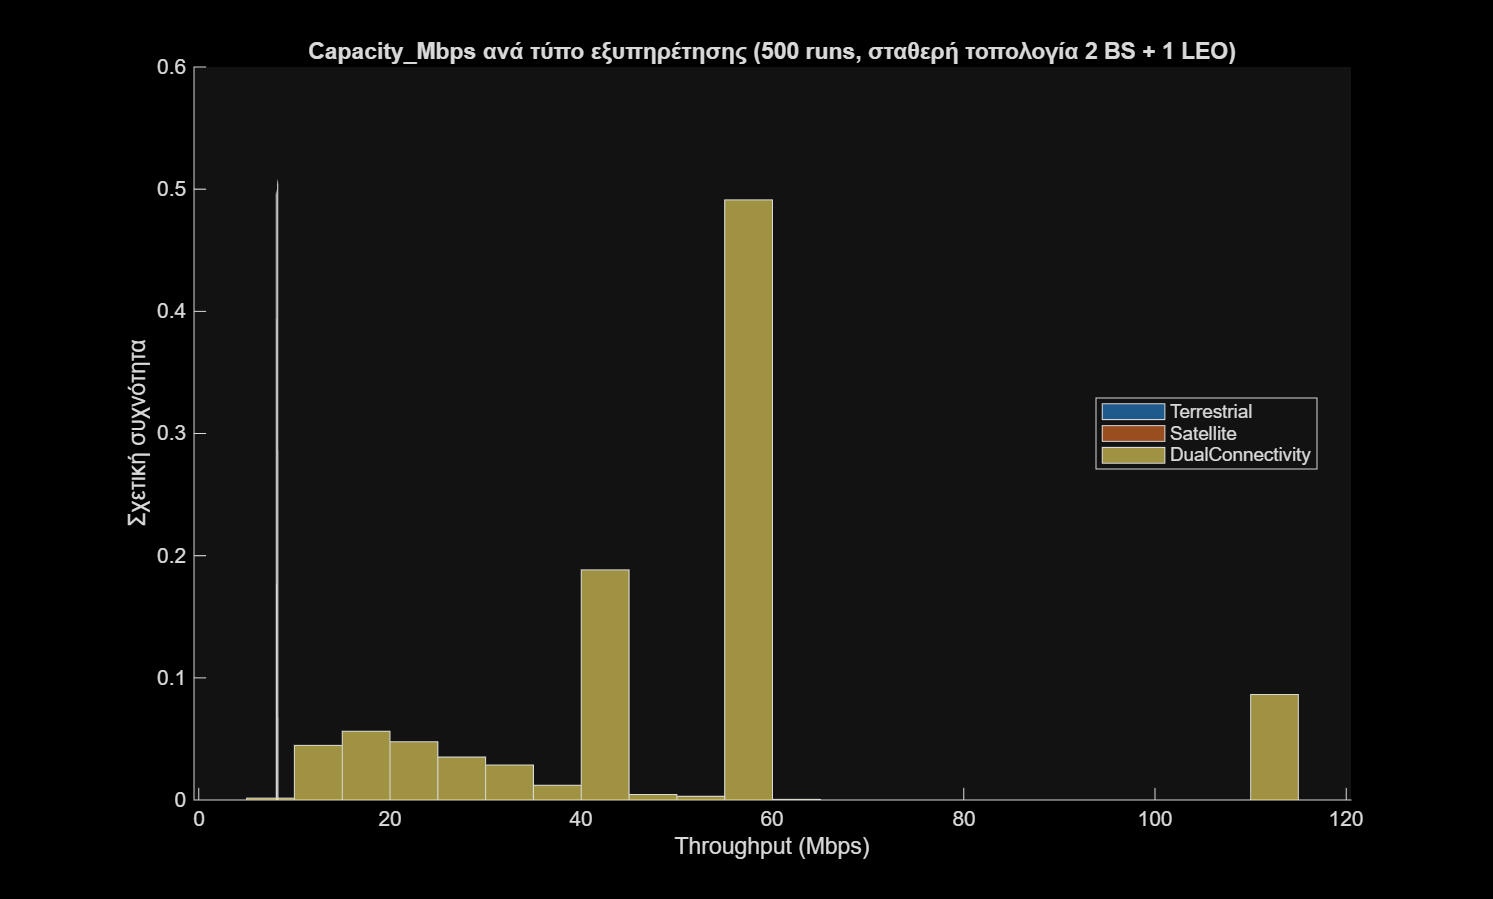
\includegraphics[width=0.75\textwidth]{kpi_hist_Capacity_Mbps.png}
\caption{Κατανομή throughput (Mbps) ανά τύπο εξυπηρέτησης, πάνω από 500 επαναλήψεις.}
\label{fig:kpi-hist-capacity}
\end{figure}

\begin{figure}[htbp]
\centering
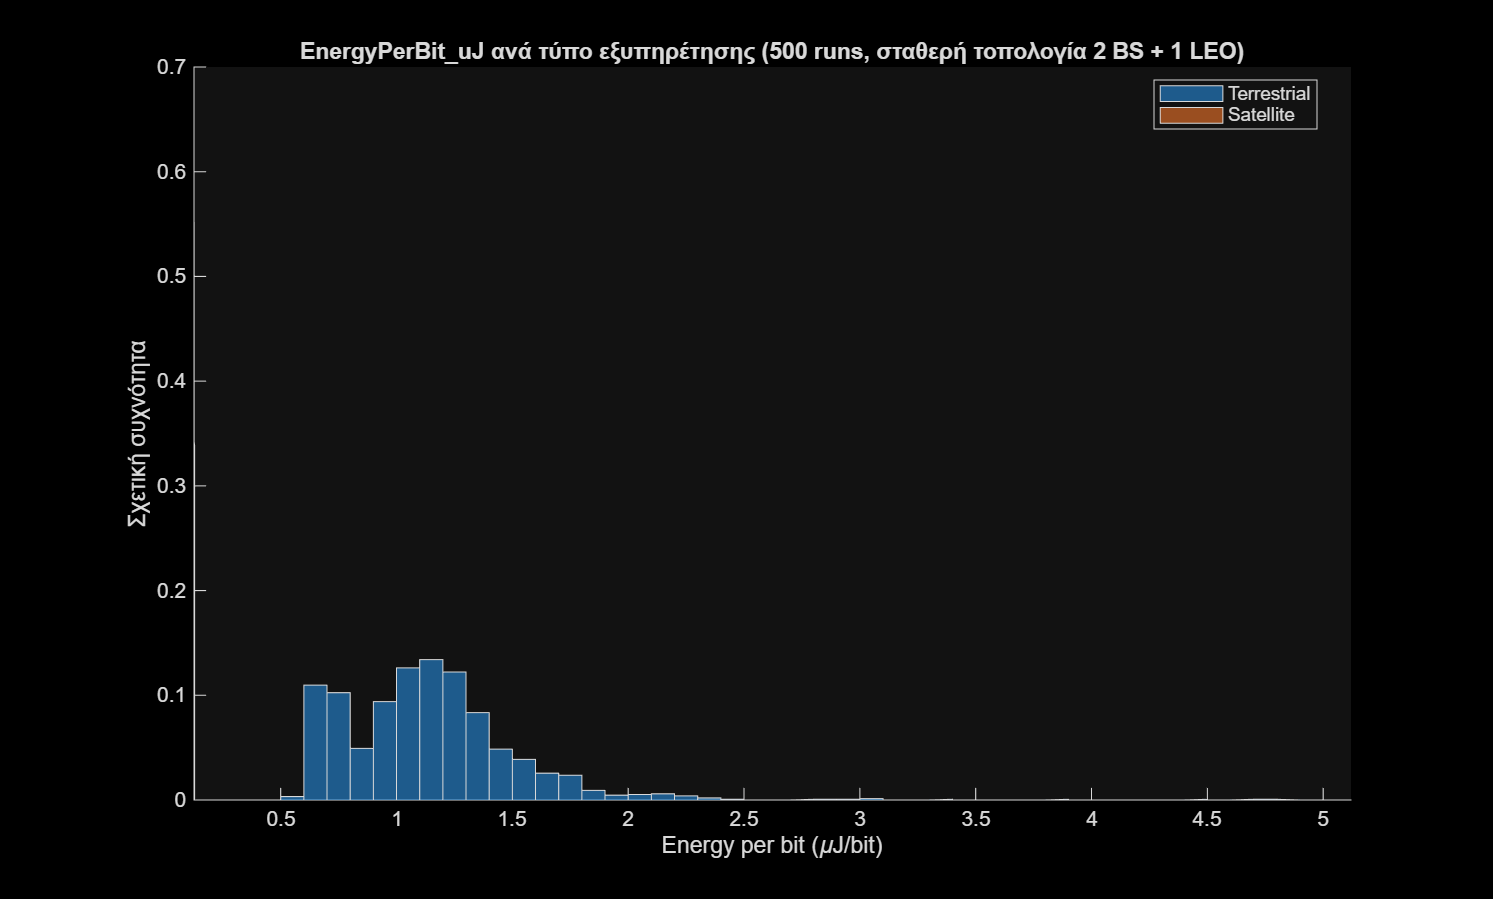
\includegraphics[width=0.75\textwidth]{kpi_hist_EnergyPerBit_uJ.png}
\caption{Κατανομή ενέργειας ανά bit (\textmu J/bit) ανά τύπο εξυπηρέτησης, πάνω από 500 επαναλήψεις.}
\label{fig:kpi-hist-energy}
\end{figure}

\begin{figure}[htbp]
\centering
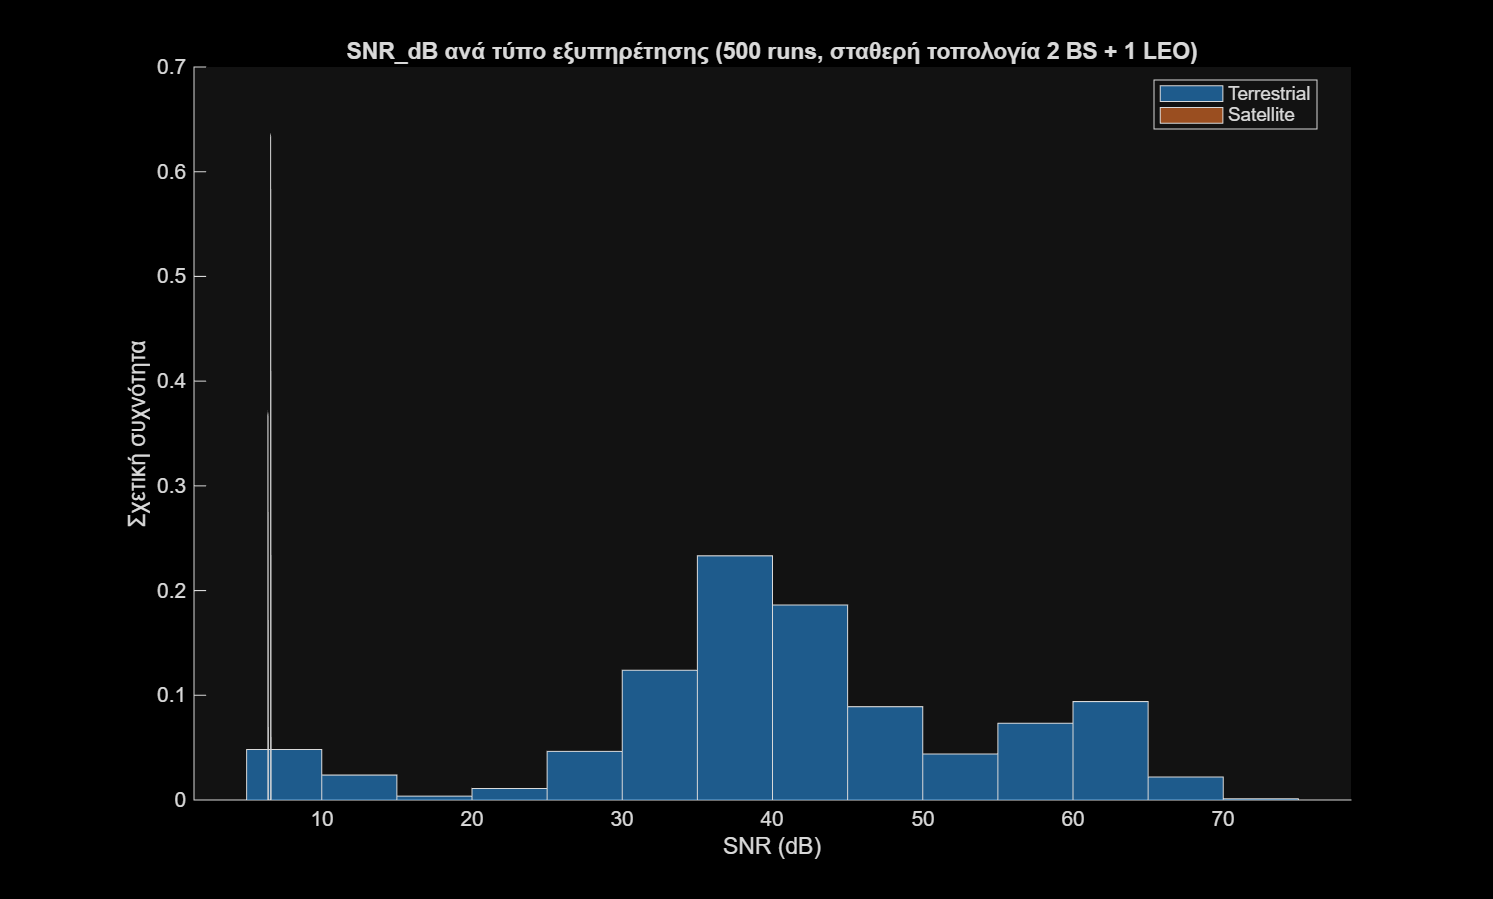
\includegraphics[width=0.75\textwidth]{kpi_hist_SNR_dB.png}
\caption{Κατανομή SNR (dB) του νικητή κόμβου, πάνω από 500 επαναλήψεις.
Μόνο η κατηγορία Satellite εμφανίζει ουσιαστική κατανομή εδώ -- ένας
DualConnectivity χρήστης δεν έχει ένα ενιαίο "SNR νικητή" (η στήλη
\texttt{SNR\_dB} είναι \texttt{NaN} για αυτές τις γραμμές, βλ.
Ενότητα~\ref{sec:meth-node-selection}), και η κατηγορία Terrestrial-only
δεν εμφανίζεται καθόλου (Πίνακας~\ref{tab:repeated-runs-summary}). Η
διακύμανση SNR ανά ζεύξη (αντί ανά νικητή) δίνεται στον
Πίνακα~\ref{tab:link-snr-std}.}
\label{fig:kpi-hist-snr}
\end{figure}

Δύο παρατηρήσεις προκύπτουν άμεσα:

\begin{itemize}
  \item \textbf{Ασύμμετρη ενεργειακή απόδοση.} Ένας Satellite-only
    χρήστης έχει $\sim\!6.3\times$ χαμηλότερο μέσο throughput από έναν
    DualConnectivity χρήστη, αλλά $\sim\!20\times$ χαμηλότερη ενέργεια
    ανά bit. Αυτό προκύπτει άμεσα από την εξίσωση~\eqref{eq:energy-per-bit}:
    η πολύ μικρότερη κατανάλωση ισχύος υποδομής του δορυφορικού payload
    (Ενότητα~\ref{sec:meth-energy}, $P_{\text{sat}} \approx 6.3$~W
    συνολικά, μοιρασμένα σε όλους τους συνδεδεμένους στον δορυφόρο --
    Satellite-only \emph{και} DualConnectivity χρήστες μαζί -- έναντι
    $P_{\text{BS}} \approx 223.8$~W ανά ενεργό BS) υπερκαλύπτει τον
    χαμηλότερο ρυθμό μετάδοσης. Ένας DualConnectivity χρήστης, αντίθετα,
    πληρώνει το ενεργειακό κόστος \emph{και} των δύο ζεύξεών του
    (εξίσωση~\eqref{eq:energy-per-bit}, άθροισμα πάνω σε
    $\mathcal{N}(u)$) για μια χωρητικότητα που κυριαρχείται σχεδόν
    αποκλειστικά από την επίγεια συνεισφορά του -- η δορυφορική ζεύξη
    προσθέτει μόλις μερικά Mbps πάνω σε δεκάδες, αλλά προσθέτει πλήρως
    το δικό της ενεργειακό μερίδιο, γι' αυτό και η ενέργεια ανά bit ενός
    DualConnectivity χρήστη ($2.61$~\textmu J/bit μέσος όρος) δεν
    διαφέρει πολύ από αυτή ενός καθαρά επίγειου χρήστη πριν την
    πολυσυνδεσιμότητα.
  \item \textbf{Ασύμμετρη διακύμανση SNR ανά ζεύξη.} Ο
    Πίνακας~\ref{tab:link-snr-std} δείχνει ότι η τυπική απόκλιση SNR στο
    επίγειο σκέλος ($19.67$~dB) είναι περίπου δύο τάξεις μεγέθους
    μεγαλύτερη από αυτή του δορυφορικού σκέλους ($0.068$~dB). Πρόκειται
    για άμεση συνέπεια της μοντελοποίησης: το επίγειο κανάλι διαθέτει
    στοχαστικό LOS/NLOS draw και shadow fading
    (εξισώσεις~\eqref{eq:los-prob-uma}-\eqref{eq:pathloss-shadowing}),
    ενώ το δορυφορικό μοντέλο (εξισώσεις~\eqref{eq:fspl}-\eqref{eq:gas-atten})
    παραμένει καθαρά ντετερμινιστικό δεδομένης της γεωμετρίας -- η
    προσθήκη της ατμοσφαιρικής απόσβεσης αερίων δεν εισάγει καμία
    στοχαστικότητα, μόνο μια μικρή, ντετερμινιστική διόρθωση. Ο δορυφόρος
    εμφανίζεται με άλλα λόγια τεχνητά "σταθερός", επειδή το μοντέλο δεν
    του αποδίδει καμία στοχαστική συνιστώσα -- ένα όριο της τρέχουσας
    μοντελοποίησης που συζητείται στο Κεφάλαιο~\ref{ch:discussion}. Αυτή
    η ίδια, μετρημένη διακύμανση είναι η πηγή του θορύβου SNR στο τρίτο
    πείραμα μηχανικής μάθησης (Ενότητα~\ref{sec:results-ml-realistic}).
\end{itemize}

\section{Χρονική εξέλιξη διέλευσης LEO}
\label{sec:results-temporal}

Η χρονική προσομοίωση (\texttt{temporalPassSimulation.m}, Ενότητα
\ref{sec:meth-temporal}) εκτέλεσε $93$ διαδοχικά χρονικά βήματα
($\Delta t = 5$~s, συνολική διάρκεια $\approx 460$~s), με το υποδορυφορικό
σημείο να κινείται με ταχύτητα $\approx 6986$~m/s (τροχιακή περίοδος
$\approx 5730$~s). Το Σχήμα~\ref{fig:temporal-elevation} δείχνει το
προκύπτον προφίλ γωνίας ανύψωσης: μια καθαρή, αναμενόμενη καμπύλη διέλευσης,
με μέγιστη γωνία ανύψωσης $\approx 89.9^\circ$ (σχεδόν ζενίθ) γύρω στα
$t \approx 215$~s.

\begin{figure}[htbp]
\centering
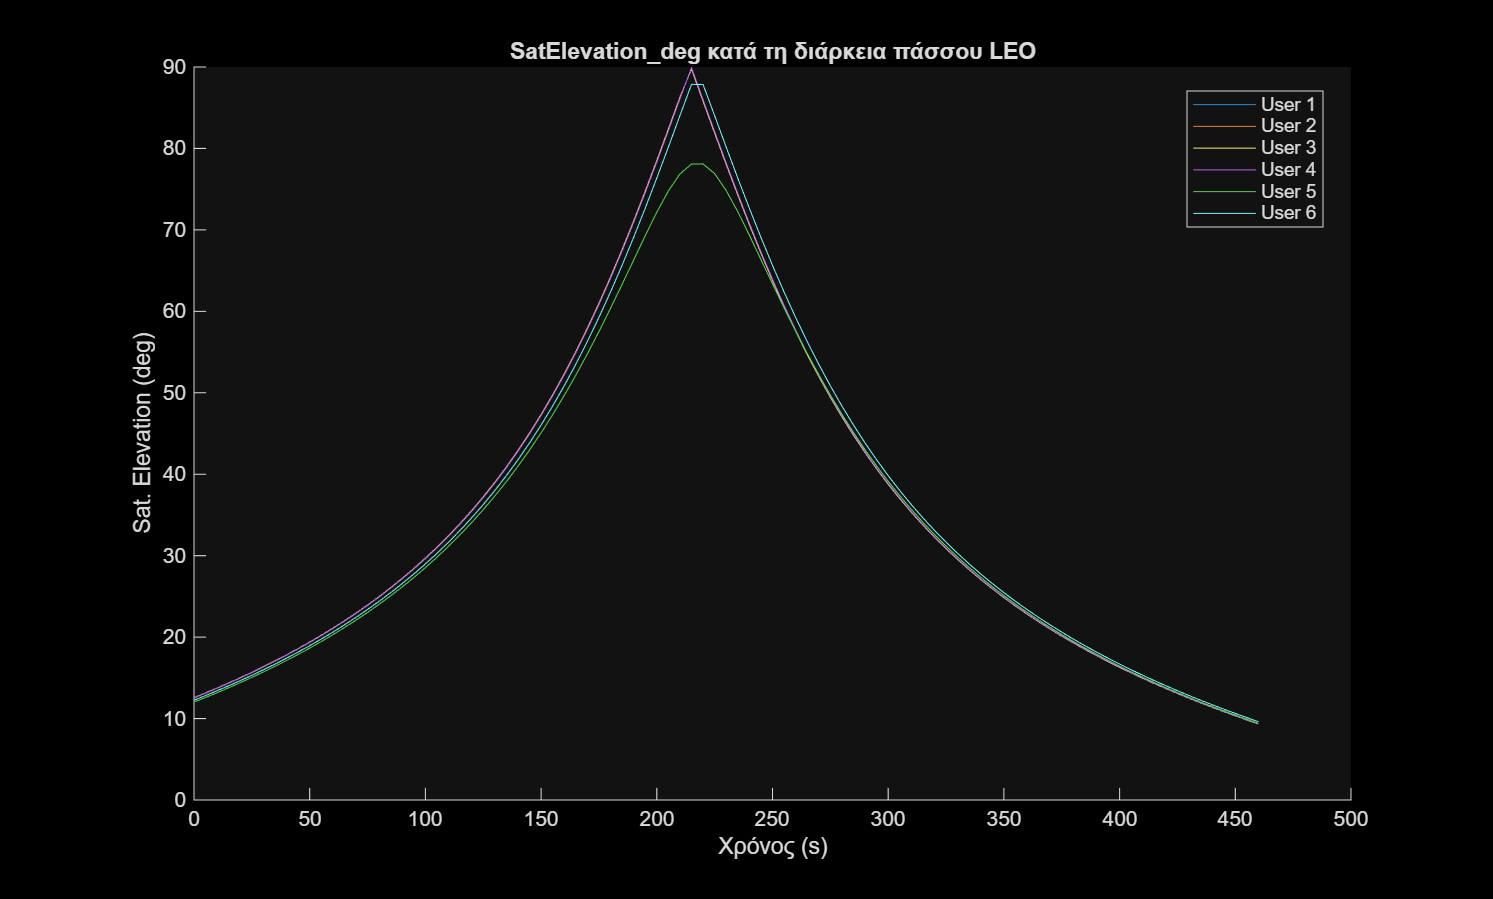
\includegraphics[width=0.8\textwidth]{temporal_SatElevation_deg.png}
\caption{Γωνία ανύψωσης δορυφόρου ανά χρήστη κατά τη διάρκεια της διέλευσης (93 βήματα, $\Delta t = 5$~s).}
\label{fig:temporal-elevation}
\end{figure}

\begin{figure}[htbp]
\centering
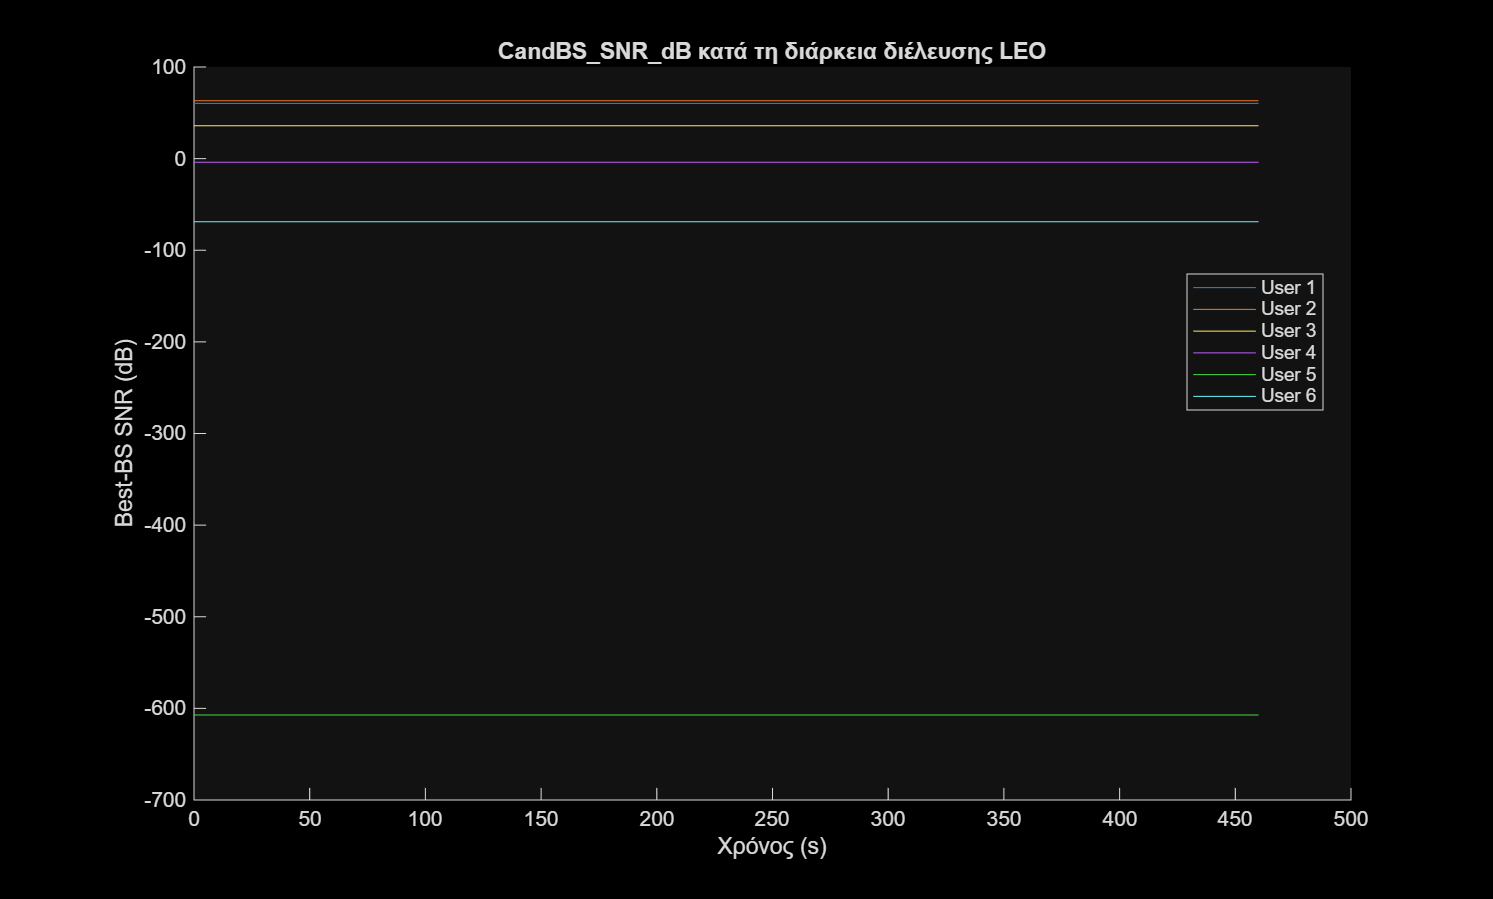
\includegraphics[width=0.8\textwidth]{temporal_CandBS_SNR_dB.png}
\caption{SNR του καλύτερου υποψήφιου BS ανά χρήστη κατά τη διάρκεια της
διέλευσης (ανεξάρτητα από το αν χρησιμοποιείται τελικά -- σταθερό, αφού
ούτε οι χρήστες ούτε οι σταθμοί βάσης μετακινούνται). Οι χρήστες $1$-$4$
έχουν σταθερά χρησιμοποιήσιμο BS SNR καθ' όλη τη διέλευση· οι χρήστες
$5$-$6$ έχουν βαθιά αρνητικό BS SNR (εκτός εμβέλειας/NLOS), πάντα κάτω
από $\text{SNR}_{\min}$.}
\label{fig:temporal-bs-snr}
\end{figure}

\begin{figure}[htbp]
\centering
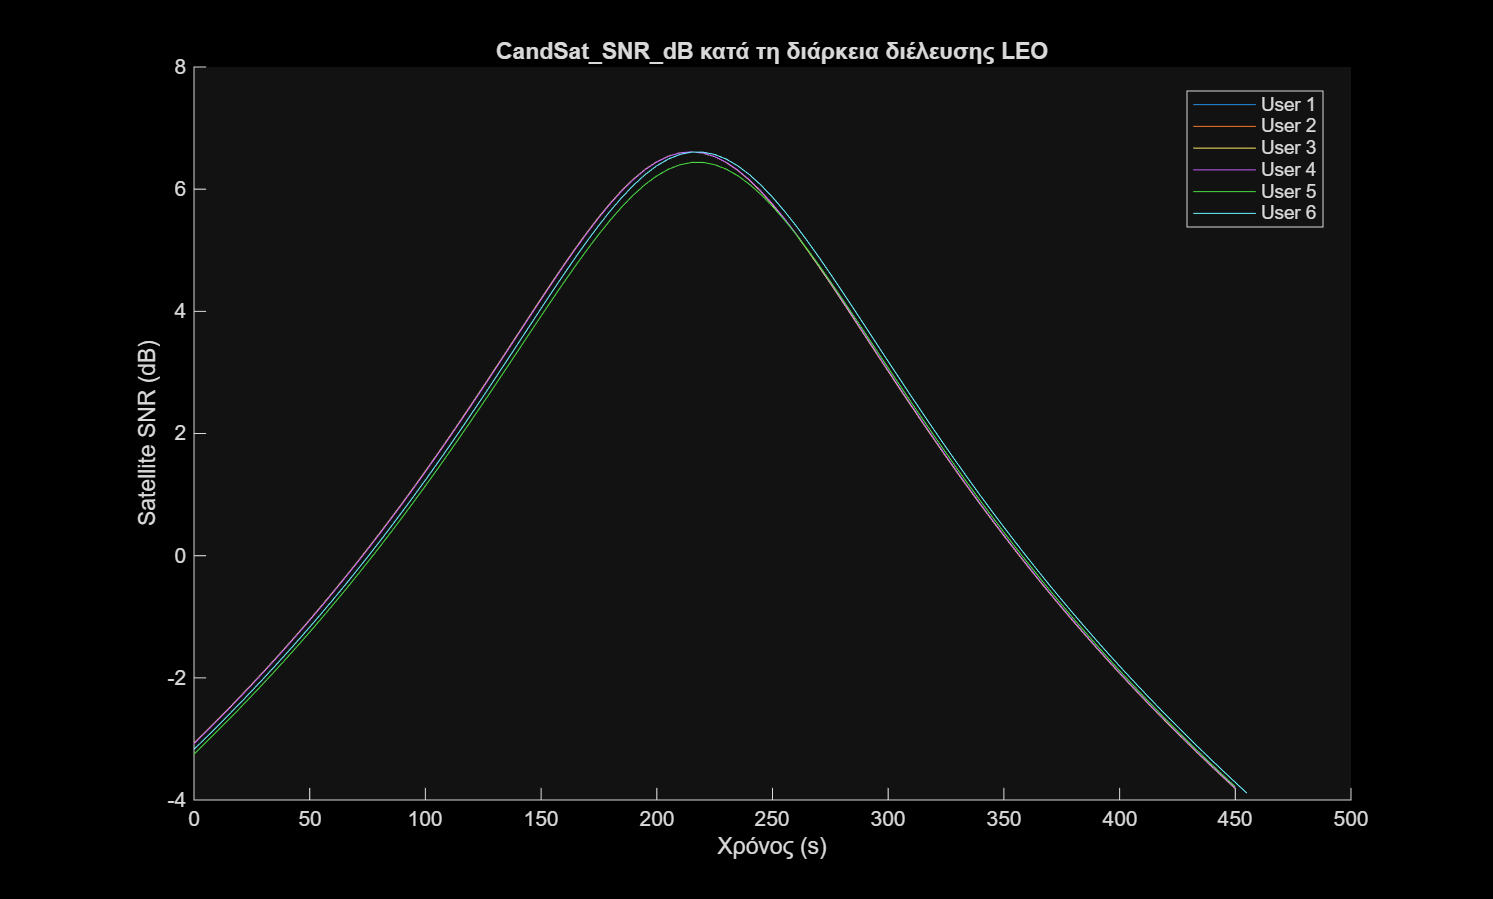
\includegraphics[width=0.8\textwidth]{temporal_CandSat_SNR_dB.png}
\caption{SNR του δορυφόρου ανά χρήστη κατά τη διάρκεια της διέλευσης
(σχεδόν ταυτόσημο και για τους $6$ χρήστες, αφού βρίσκονται όλοι κοντά
μεταξύ τους σε σχέση με το υψόμετρο του δορυφόρου). Η γραμμή διακόπτεται
όποτε ο δορυφόρος είναι εκτός ορατότητας
($\text{SNR}_{\text{sat}} = -\infty$). Η μετάβαση κάτω από
$\text{SNR}_{\min} \approx -7.53$~dB προς το τέλος της διέλευσης οδηγεί
τους χρήστες $1$-$4$ σε SN event (αποβολή του δορυφόρου, παραμονή στο
BS) και τους χρήστες $5$-$6$ σε ρητή κατάσταση outage
(Ενότητα~\ref{subsec:results-outage}).}
\label{fig:temporal-sat-snr}
\end{figure}

\subsection{Handovers, SN events και outage events}
\label{subsec:results-handovers}

Ο Πίνακας~\ref{tab:handovers} καταγράφει τρεις ξεχωριστούς τύπους
μετάβασης ανά χρήστη κατά τη διάρκεια της διέλευσης: \emph{handover}
(αλλάζει ο σταθμός βάσης -- ο "master node" MN, στην ορολογία MR-DC του
Majamaa~\cite{majamaa2024toward} που ήδη αναφέρθηκε στο
Κεφάλαιο~\ref{ch:background}), \emph{SN event} (προστίθεται ή αφαιρείται
ο δορυφόρος -- ο "secondary node" SN -- ενώ ο MN παραμένει ο ίδιος), και
\emph{outage event} (μετάβαση προς \texttt{ServingNode="None"}). Η
διάκριση αυτή είναι απαραίτητη μετά την πολυσυνδεσιμότητα
(εξίσωση~\eqref{eq:node-selection}): μια μετάβαση
DualConnectivity$\rightarrow$Terrestrial δεν αλλάζει τον σταθμό βάσης
που εξυπηρετεί τον χρήστη, οπότε δεν είναι πραγματικό handover, παρότι η
τιμή του \texttt{ServingType} αλλάζει.

\begin{table}[htbp]
\centering
\caption{Αριθμός handovers, SN events και outage events ανά χρήστη κατά
τη διάρκεια της διέλευσης (93 διαδοχικά βήματα), με το χωρικά
συσχετισμένο μοντέλο shadow fading (εξίσωση~\eqref{eq:correlated-sf}),
πολυσυνδεσιμότητα και ρητή κατάσταση outage
(εξίσωση~\eqref{eq:node-selection}).}
\label{tab:handovers}
\begin{tabular}{@{}c c c c c c@{}}
\toprule
User & Handovers & SN events & Outage events & Αρχικός κόμβος & Τελικός κόμβος \\
\midrule
1 & 0 & 1 & 0 & BS2+SAT-1 & BS2 \\
2 & 0 & 1 & 0 & BS2+SAT-1 & BS2 \\
3 & 0 & 1 & 0 & BS1+SAT-1 & BS1 \\
4 & 0 & 1 & 0 & BS2+SAT-1 & BS2 \\
5 & 0 & 0 & 1 & SAT-1     & None (outage) \\
6 & 0 & 0 & 1 & SAT-1     & None (outage) \\
\bottomrule
\end{tabular}
\end{table}

Η εικόνα εδώ διαφέρει σημαντικά από αυτή που έδινε τόσο το αρχικό,
ανεξάρτητο-ανά-βήμα μοντέλο σκίασης, όσο και το προγενέστερο,
single-connectivity μοντέλο επιλογής κόμβου. Δεν καταγράφεται \emph{κανένα}
πραγματικό handover: οι χρήστες $1$-$4$ (κοντά σε σταθμό βάσης καθ' όλη τη
διέλευση) διατηρούν σταθερά τον ίδιο "master" σταθμό βάσης, κάτι
αναμενόμενο αφού ούτε οι ίδιοι ούτε οι σταθμοί βάσης μετακινούνται· δεν
υπάρχει δηλαδή φυσικός λόγος να αλλάζει ο νικητής BS1/BS2 ανά βήμα, και το
συσχετισμένο μοντέλο πλέον το αντικατοπτρίζει σωστά. Αντ' αυτού, οι
χρήστες $1$-$4$ ξεκινούν \emph{ήδη} σε DualConnectivity (το BS SNR τους
είναι σταθερά αρκετά καλό, Σχήμα~\ref{fig:temporal-bs-snr}, ενώ ο
δορυφόρος είναι ήδη ορατός/χρησιμοποιήσιμος από την αρχή της διέλευσης,
Σχήμα~\ref{fig:temporal-sat-snr}) και καταλήγουν σε Terrestrial-only μόνο
όταν ο δορυφόρος βγαίνει εκτός ορατότητας στο τέλος -- μια \emph{αφαίρεση
δευτερεύοντος κόμβου} (SN event), όχι handover: ο σταθμός βάσης που τους
εξυπηρετεί δεν αλλάζει ποτέ. Οι χρήστες $5$-$6$ (πολύ μακριά από κάθε
σταθμό βάσης, BS SNR πάντα βαθιά κάτω από $\text{SNR}_{\min}$) χάνουν την
ίδια ορατότητα δορυφόρου προς το τέλος της διέλευσης, αλλά, δίχως ποτέ
κανέναν χρησιμοποιήσιμο επίγειο υποψήφιο, καταλήγουν σε ρητή κατάσταση
outage αντί σε Terrestrial-only (βλ. Ενότητα~\ref{subsec:results-outage}).
Αυτή η διαφοροποίηση -- ίδιο γεγονός στον δορυφόρο (απώλεια ορατότητας),
διαφορετική έκβαση ανάλογα με το αν υπάρχει χρησιμοποιήσιμος επίγειος
υποψήφιος -- είναι η αναμενόμενη, φυσικά ερμηνεύσιμη συμπεριφορά ενός
ρεαλιστικού κανόνα επιλογής κόμβου. Η σύγκριση με το αρχικό, ασυσχέτιστο
μοντέλο σκίασης (όπου οι ίδιοι χρήστες εμφάνιζαν έως και $29$ handovers
μέσα σε $460$~s) επιβεβαιώνει ότι το τεχνητά συχνό ping-pong της
Ενότητας~\ref{sec:meth-temporal} ήταν πράγματι μεθοδολογικό τεχνούργημα
(artifact) του ανεξάρτητου δειγματισμού σκίασης και όχι φυσικό φαινόμενο,
και ότι διορθώνεται πλήρως με τη χωρική συσχέτιση κατά
Gudmundson~\cite{gudmundson1991correlation}.

\subsection{Ρητή κατάσταση outage}
\label{subsec:results-outage}

Ένα δεύτερο εύρημα εντοπίστηκε αρχικά στο τέλος της διέλευσης, όταν η
γωνία ανύψωσης του δορυφόρου έπεφτε κάτω από το όριο ορατότητας για τους
απομακρυσμένους χρήστες. Στα βήματα $92$-$93$ ($t = 455$-$460$~s), ο
χρήστης $5$, σε απόσταση $\sim\!107$~km από τον πλησιέστερο σταθμό
βάσης, με γωνία ανύψωσης δορυφόρου κάτω από $10^\circ$ (οριακά εκτός
ορατότητας), αναγκαζόταν από τον αρχικό κανόνα -- ένα καθαρό $\argmax$
χωρίς κατώφλι ελάχιστης αποδεκτής ποιότητας -- να ανατεθεί στον
"καλύτερο" επίγειο υποψήφιο, ο οποίος όμως είχε:
\[
\text{PathLoss} = 754.6\text{~dB}, \qquad \text{SNR} = -607.2\text{~dB},
\qquad \text{Capacity} \to 0, \qquad \text{Energy/bit} \to \infty.
\]
Το να "εξυπηρετείται" επίσημα ένας χρήστης από έναν κόμβο με μηδενική
πρακτική χρησιμότητα δεν ήταν σφάλμα υλοποίησης, αλλά άμεση συνέπεια της
απουσίας κατωφλίου στον αρχικό κανόνα επιλογής: επέλεγε πάντα τον
"λιγότερο κακό" υποψήφιο, ακόμα κι όταν κανένας δεν ήταν στην
πραγματικότητα χρησιμοποιήσιμος. Κάτι τέτοιο δεν θα μπορούσε να
παρατηρηθεί στο στατικό σενάριο αναφοράς (Ενότητα~\ref{sec:results-static}),
όπου η γεωμετρία επιλέχθηκε ώστε ο δορυφόρος να παραμένει πάντα ορατός με
άνεση περιθωρίου -- εδώ φάνηκε η αξία της χρονικής προσομοίωσης ως
εργαλείου εντοπισμού ορίων του μοντέλου.

Το εύρημα αυτό αντιμετωπίστηκε ήδη εντός του Μέρους~1, με την προσθήκη
του κατωφλίου $\text{SNR}_{\min} \approx -7.53$~dB στον κανόνα επιλογής
κόμβου (εξίσωση~\eqref{eq:node-selection}, Ενότητα~\ref{sec:meth-node-selection}).
Ξανατρέχοντας την ίδια ακριβώς διέλευση με τον διορθωμένο κανόνα, ο
χρήστης $5$ (και ομοίως ο χρήστης $6$) καταγράφεται πλέον σωστά ως
\texttt{ServingNode="None"} / \texttt{ServingType="Outage"} στα βήματα
$92$-$93$ (Πίνακας~\ref{tab:handovers}) αντί να ανατεθεί στο ανύπαρκτο
BS2: η χωρητικότητα γίνεται ρητά $0$ (όχι απλώς αριθμητικά αμελητέα λόγω
του σχεδόν μηδενικού SNR) και δεν αποδίδεται καθόλου κατανάλωση ισχύος σε
έναν κόμβο που στην πραγματικότητα δεν εξυπηρετεί κανέναν. Τα διαγνωστικά
του "καλύτερου" (αλλά μη-χρησιμοποιήσιμου) υποψηφίου -- ίδιο
$\text{PathLoss} = 754.6$~dB, $\text{SNR} = -607.2$~dB όπως παραπάνω --
παραμένουν διαθέσιμα στην έξοδο για ανάλυση, απλά δεν καθορίζουν πλέον
μια ψευδή ανάθεση εξυπηρέτησης. Σημειώνεται ότι ο χρήστης $4$, σε
αντίστοιχη απόσταση από τον δορυφόρο, \emph{δεν} καταλήγει σε outage
(Ενότητα~\ref{subsec:results-handovers}) -- έχει έναν επίγειο υποψήφιο
αρκετά καλό ώστε να ξεπερνά το $\text{SNR}_{\min}$ σε όλη τη διάρκεια
της διέλευσης, οπότε παραμένει απλώς εξυπηρετούμενος από τον σταθμό
βάσης (μια αφαίρεση δευτερεύοντος κόμβου, όχι απώλεια κάλυψης) όταν ο
δορυφόρος γίνεται αόρατος. Η διαφοροποίηση αυτή είναι ακριβώς το
ζητούμενο: το μοντέλο πλέον διακρίνει "υπάρχει κάλυψη έστω και από μία
μόνο ζεύξη" από "δεν υπάρχει καθόλου κάλυψη", αντί να τα συγχέει.

\section{Αποτελέσματα πρώτου μοντέλου μηχανικής μάθησης}
\label{sec:results-ml}

Πάνω σε ένα σύνολο δεδομένων $200$ τυχαιοποιημένων σεναρίων
($1313$ γραμμές χρηστών, \texttt{rng(42)}) που παρήγαγε ο
\texttt{monteCarloDriver.m} (Ενότητα~\ref{sec:meth-montecarlo}, το
τεκμηριωμένο default του driver), τα δύο μοντέλα της
Ενότητας~\ref{sec:meth-ml} πέτυχαν τις επιδόσεις του
Πίνακα~\ref{tab:ml-results} (grouped split 961/352 γραμμών σε
150/50 σενάρια εκπαίδευσης/ελέγχου). Η κατανομή κλάσεων στο σύνολο
δεδομένων είναι $0\%$ Terrestrial-only, $32\%$ Satellite, $68\%$
DualConnectivity -- η κατηγορία Terrestrial-only \emph{δεν εμφανίζεται
καθόλου}, αφού η ίδια η δορυφορική γεωμετρία/κάλυψη του σεναρίου κάνει
τον δορυφόρο σχεδόν πάντα ταυτόχρονα χρησιμοποιήσιμο όποτε είναι
χρησιμοποιήσιμος και ο επίγειος υποψήφιος (βλ. συζήτηση στο τέλος αυτής
της ενότητας). Οι μετρικές F1/ROC-AUC υπολογίζονται macro-averaged πάνω
στις κλάσεις που όντως εμφανίζονται στο test set (Terrestrial-only
εξαιρείται αυτόματα, αφού έχει μηδενική υποστήριξη παντού).

\begin{table}[htbp]
\centering
\caption{Επιδόσεις πρόβλεψης \texttt{ServingType} (Terrestrial/
Satellite/DualConnectivity), grouped train/test split ανά
\texttt{ScenarioID} (75/25).}
\label{tab:ml-results}
\begin{tabular}{@{}l c c c@{}}
\toprule
Μοντέλο & Accuracy & F1 (macro) & ROC-AUC (macro, OvR) \\
\midrule
Λογιστική Παλινδρόμηση & 0.9858 & 0.9840 & 0.9993 \\
Random Forest          & 0.9972 & 0.9968 & 1.0000 \\
\bottomrule
\end{tabular}
\end{table}

\begin{figure}[htbp]
\centering
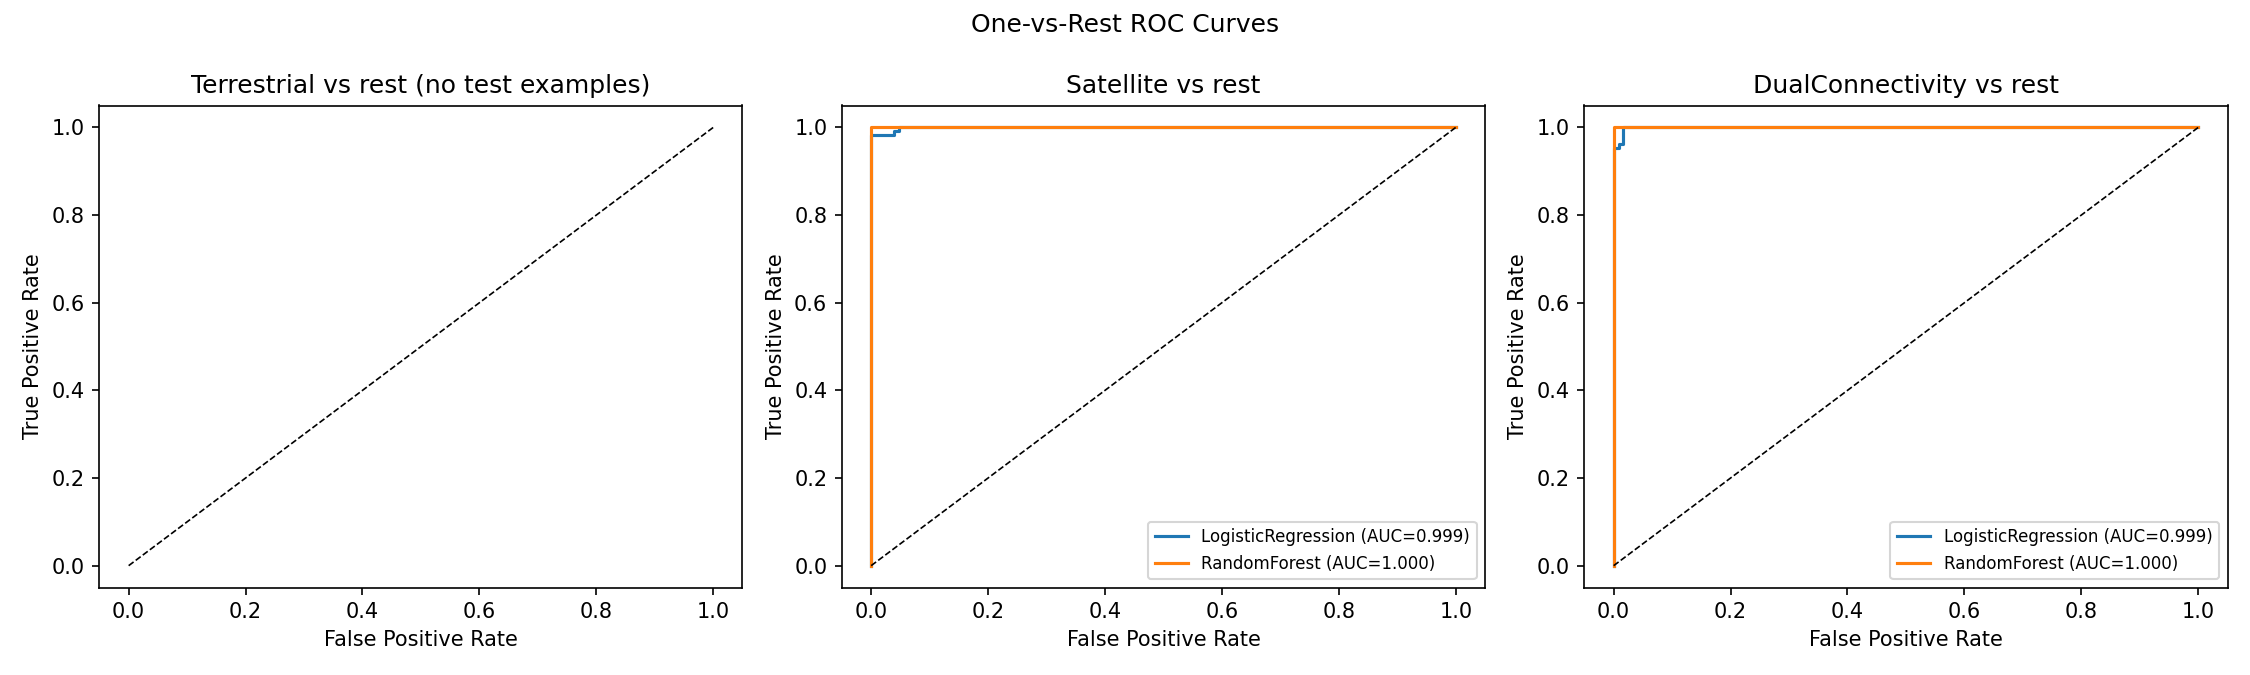
\includegraphics[width=\textwidth]{roc_curve.png}
\caption{One-vs-rest καμπύλες ROC για τα δύο μοντέλα, ανά κλάση. Το
υποπλαίσιο Terrestrial δεν έχει καμπύλες, αφού η κλάση αυτή δεν
εμφανίζεται στο test set.}
\label{fig:ml-roc}
\end{figure}

\begin{figure}[htbp]
\centering
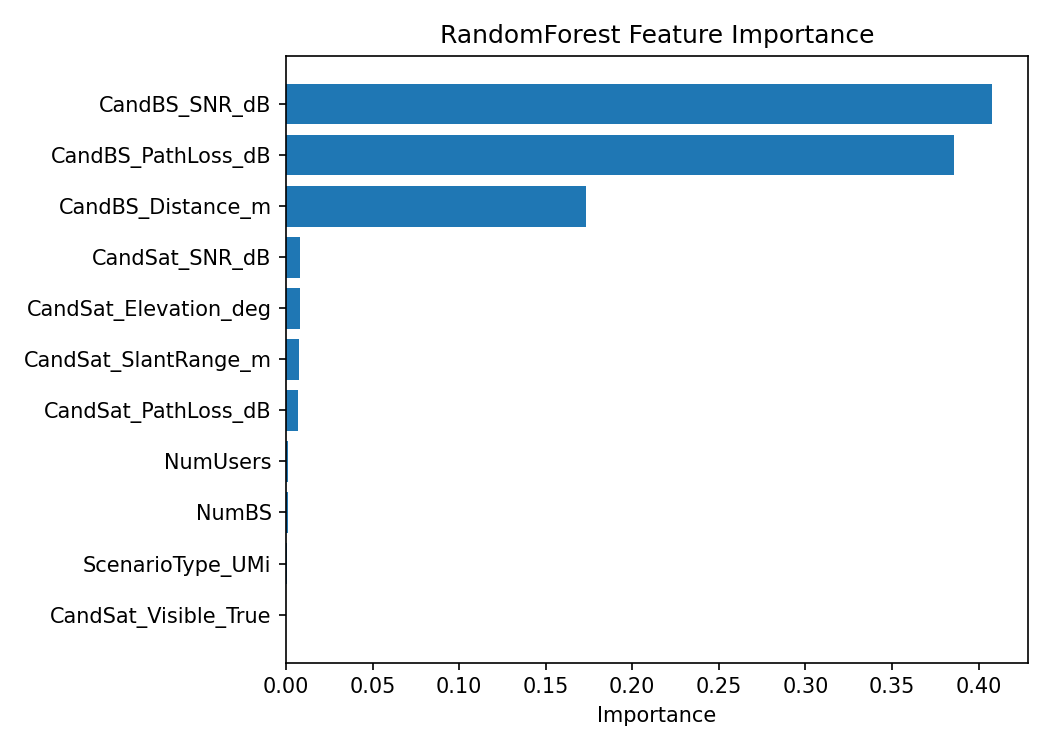
\includegraphics[width=0.7\textwidth]{feature_importance_RandomForest.png}
\caption{Σπουδαιότητα χαρακτηριστικών (Random Forest). Τα δύο υποψήφια SNR
κυριαρχούν, όπως αναμενόταν από τον κανόνα κατωφλίου της
εξίσωσης~\eqref{eq:node-selection}.}
\label{fig:ml-feature-importance}
\end{figure}

Το Random Forest παραμένει, όπως προβλέφθηκε στην
Ενότητα~\ref{sec:meth-ml}, ουσιαστικά τέλειο ($99.72\%$ Accuracy,
$100\%$ ROC-AUC): αναμενόμενη συνέπεια του ότι η ίδια η ετικέτα ορίζεται
σχεδόν ντετερμινιστικά από δύο από τα χαρακτηριστικά εισόδου
(\texttt{CandBS\_SNR\_dB}, \texttt{CandSat\_SNR\_dB}), κάτι που
επιβεβαιώνεται και από το Σχήμα~\ref{fig:ml-feature-importance}, όπου τα
δύο αυτά χαρακτηριστικά κυριαρχούν σαφώς έναντι όλων των υπολοίπων. Η
Λογιστική Παλινδρόμηση πλησιάζει πλέον πολύ κοντά ($98.58\%$ Accuracy) --
σε αντίθεση με το αρχικό, δυαδικό πείραμα πριν την πολυσυνδεσιμότητα,
όπου η Λογιστική Παλινδρόμηση υστερούσε αισθητά ($88.35\%$): με τρεις
κλάσεις αντί για δύο, και με την DualConnectivity κλάση να είναι πλέον η
πλειοψηφική ($68\%$), το πρόβλημα ταξινόμησης είναι σε γενικές γραμμές
ευκολότερο για ένα γραμμικό μοντέλο, αφού η κυρίαρχη κλάση είναι και η
πιο εύκολα διαχωρίσιμη (ξεπερνά και τα δύο κατώφλια SNR ταυτόχρονα). Η
αξία αυτού του πρώτου πειράματος βρίσκεται συνεπώς αμιγώς στην
επαλήθευση ορθότητας του συνολικού pipeline δεδομένων
(Ενότητα~\ref{sec:impl-dataflow}), όχι σε απόδειξη ότι το πρόβλημα
πρόβλεψης connectivity είναι εύκολο -- βλ. την επόμενη ενότητα για το πώς
αυτό ερμηνεύεται μαζί με τα άλλα δύο πειράματα.

\section{Προς ρεαλιστικότερα σενάρια πρόβλεψης}
\label{sec:results-ml-realistic}

Το πείραμα της προηγούμενης ενότητας δίνει στο μοντέλο κάτι που ένα
πραγματικό σύστημα δεν θα είχε ποτέ: το ακριβές, στιγμιαίο SNR ενός
υποψήφιου κόμβου με τον οποίο ο χρήστης δεν έχει καν συνδεθεί ακόμα. Για
να εκτιμηθεί πόσο από την υψηλή απόδοση του Πίνακα~\ref{tab:ml-results}
οφείλεται σε αυτή την "κλειδωμένη" πληροφορία, εκπαιδεύτηκαν δύο ακόμα
παραλλαγές των ίδιων δύο ταξινομητών, πάνω στο ίδιο σύνολο δεδομένων και
grouped split, με προοδευτικά λιγότερη πληροφορία SNR. Οι τρεις
παραλλαγές δεν υπάρχουν απλώς για σύγκριση μεταξύ τους -- έχουν η καθεμία
συγκεκριμένο ρόλο: το ακριβές SNR είναι \emph{έλεγχος ορθότητας} του
pipeline (Ενότητα~\ref{sec:bg-ml}), όχι πρόβλεψη προς αναφορά· η
\textbf{μόνο-γεωμετρία} παραλλαγή είναι ένα \emph{κατώτατο όριο} (τι θα
πετύχαινε ένα μοντέλο χωρίς καμία μέτρηση σήματος)· και η
\textbf{θορυβώδης-SNR} παραλλαγή είναι αυτή που η παρούσα εργασία θεωρεί
\emph{αντιπροσωπευτική μιας πραγματικής ανάπτυξης}, αφού προσεγγίζει τι θα
είχε στη διάθεσή του ένα πραγματικό σύστημα (μέτρηση, όχι τέλεια γνώση,
αλλά ούτε πλήρης απουσία σήματος) -- και είναι το αποτέλεσμα στο οποίο
βασίζονται τα συμπεράσματα των Κεφαλαίων~\ref{ch:discussion}
και~\ref{ch:conclusions} όπου αναφέρεται απόδοση πρόβλεψης.

\begin{itemize}
  \item \textbf{Θορυβώδες SNR.} Τα \texttt{CandBS\_SNR\_dB}/
    \texttt{CandSat\_SNR\_dB} παραμένουν χαρακτηριστικά, αλλά πριν
    δοθούν στο μοντέλο προστίθεται σε καθένα ανεξάρτητος γκαουσιανός
    θόρυβος, ώστε να αναπαρασταθεί μια ελαφρώς παλαιωμένη/ατελής μέτρηση
    αντί της ακριβούς τρέχουσας τιμής -- πιο κοντά σε ό,τι θα είχε στη
    διάθεσή του ένα πραγματικό UE μέσω περιοδικών αναφορών μέτρησης
    γειτονικών κυψελών (π.χ. Event A3/A5, TS~38.331) παρά η τέλεια,
    στιγμιαία τιμή του προηγούμενου πειράματος. Η τυπική απόκλιση του
    θορύβου δεν επινοήθηκε: είναι η \emph{πραγματική, μετρημένη}
    διακύμανση SNR ανά ζεύξη από τα $500$ επαναλαμβανόμενα runs της
    Ενότητας~\ref{sec:results-repeated} (Πίνακας~\ref{tab:link-snr-std})
    -- $19.6721$~dB για το επίγειο σκέλος, $0.0682$~dB για το δορυφορικό
    (μικρή τιμή επειδή το δορυφορικό κανάλι εδώ είναι ντετερμινιστικό
    δεδομένης της γεωμετρίας -- βλ. Ενότητα~\ref{sec:meth-sat-channel}).
  \item \textbf{Μόνο γεωμετρία.} Αφαιρούνται εντελώς τα δύο SNR
    χαρακτηριστικά, \emph{και} τα δύο χαρακτηριστικά path loss
    (\texttt{CandBS\_PathLoss\_dB}/\texttt{CandSat\_PathLoss\_dB}), αφού
    το path loss είναι σχεδόν affine συνάρτηση του SNR δεδομένου
    σταθερού EIRP/θορύβου ανά τύπο κόμβου (εξισώσεις~\eqref{eq:snr-bs},
    \eqref{eq:snr-sat}) -- η διατήρησή του θα ξανάφερνε το ίδιο
    "shortcut" υπό άλλο όνομα. Μένουν μόνο \texttt{CandBS\_Distance\_m},
    \texttt{CandSat\_Elevation\_deg}, \texttt{CandSat\_SlantRange\_m},
    \texttt{CandSat\_Visible}, και το context (\texttt{NumBS},
    \texttt{NumUsers}, \texttt{ScenarioType}) -- ό,τι θα ήταν γνωστό σε
    ένα σύστημα \emph{πριν} από οποιαδήποτε μέτρηση σήματος.
\end{itemize}

\begin{table}[htbp]
\centering
\caption{Επιδόσεις πρόβλεψης \texttt{ServingType} με προοδευτικά λιγότερη
πληροφορία SNR (ίδιο dataset/split με τον Πίνακα~\ref{tab:ml-results}).}
\label{tab:ml-results-realistic}
\small
\begin{tabular}{@{}l c c c c@{}}
\toprule
Χαρακτηριστικά εισόδου & LR Accuracy & LR ROC-AUC & RF Accuracy & RF ROC-AUC \\
\midrule
Ακριβές SNR (Πίνακας~\ref{tab:ml-results})  & 0.9858 & 0.9993 & 0.9972 & 1.0000 \\
Θορυβώδες SNR                                & 0.9858 & 0.9973 & 0.9915 & 0.9965 \\
Μόνο γεωμετρία (χωρίς SNR)                   & 0.9830 & 0.9859 & 0.9915 & 0.9902 \\
\bottomrule
\end{tabular}
\end{table}

\begin{figure}[htbp]
\centering
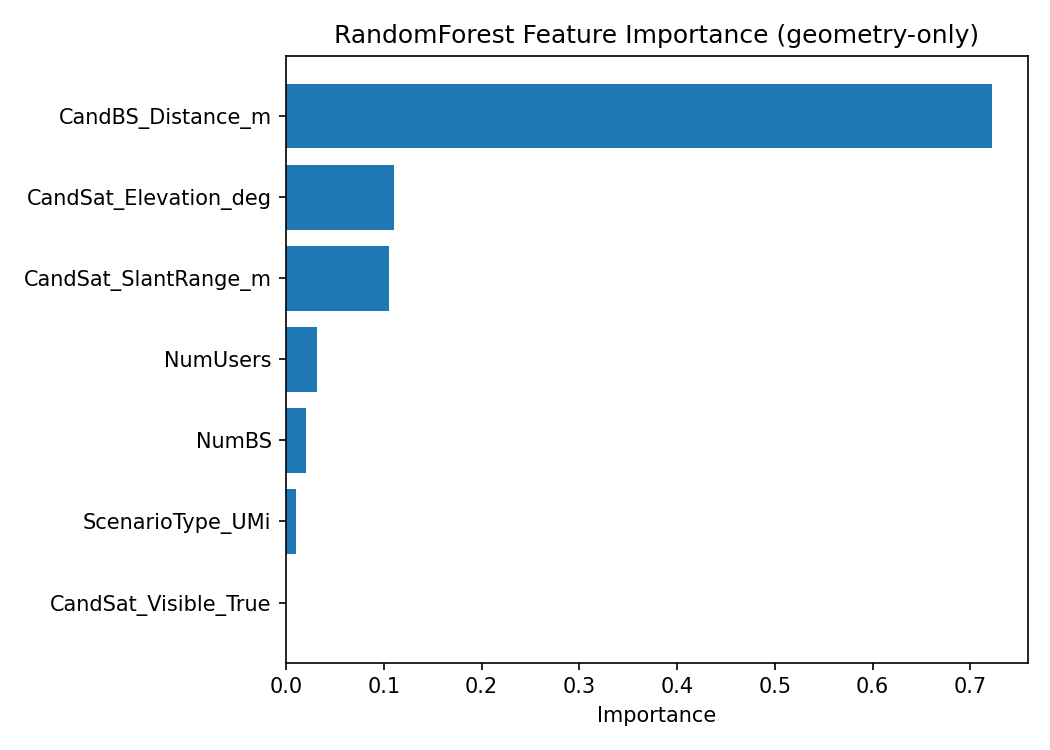
\includegraphics[width=0.7\textwidth]{feature_importance_RandomForest_geometry_only.png}
\caption{Σπουδαιότητα χαρακτηριστικών (Random Forest, μόνο γεωμετρία --
χωρίς SNR ή path loss). Η απόσταση προς το καλύτερο BS κυριαρχεί, αφού
είναι πλέον το χαρακτηριστικό που καθορίζει σχεδόν αποκλειστικά αν ένας
χρήστης είναι Satellite-only ή DualConnectivity -- βλ. συζήτηση παρακάτω.}
\label{fig:ml-feature-importance-geo}
\end{figure}

Το πρώτο πράγμα που ξεχωρίζει στον Πίνακα~\ref{tab:ml-results-realistic}
είναι αυτό \emph{που δεν συμβαίνει}: δεν υπάρχει πια η καθαρή, μονότονη
πτώση Accuracy που θα περίμενε κανείς καθώς αφαιρείται πληροφορία SNR.
Το Random Forest πιάνει $99.15\%$ και στα δύο πειράματα μειωμένης
πληροφορίας -- \emph{το ίδιο} ποσοστό στο θορυβώδες SNR όσο και στη μόνο
γεωμετρία -- ενώ ακόμα και η Λογιστική Παλινδρόμηση μένει πάνω από
$98\%$ και στα τρία πειράματα. Πριν την πολυσυνδεσιμότητα, το ίδιο αυτό
πείραμα έδειχνε μια σαφή, τρίβημη σκάλα ($100\% \rightarrow 89.5\%
\rightarrow 87.2\%$ Accuracy για το Random Forest): η αιτία της
διαφοράς δεν είναι σφάλμα στην υλοποίηση της αξιολόγησης (η μάσκα σε
κλάσεις παρούσες στο test set, Ενότητα~\ref{sec:meth-ml}, ελέγχθηκε
ρητά ώστε να μην κρύβει τεχνητά μια πτώση), αλλά μια πραγματική συνέπεια
της αλλαγής της ίδιας της ετικέτας: αφού η κατηγορία Terrestrial-only
εξαφανίστηκε από το dataset (Ενότητα~\ref{sec:results-ml}), το πρόβλημα
τριών κλάσεων ανάγεται ουσιαστικά σε \emph{DualConnectivity έναντι
Satellite-only} -- και αυτή η διάκριση εξαρτάται σχεδόν αποκλειστικά από
το αν ο χρήστης τοποθετήθηκε "κοντά" ή "μακριά" από σταθμό βάσης στη
γεννήτρια Monte Carlo (Ενότητα~\ref{sec:meth-montecarlo}: πιθανότητα
$30\%$ για "μακρινό" χρήστη, με ακτίνα $1$-$150$~km), \emph{όχι} από μια
λεπτή διαφορά SNR μεταξύ δύο κοντινών υποψηφίων. Η απόσταση BS από μόνη
της (Σχήμα~\ref{fig:ml-feature-importance-geo}) κωδικοποιεί σχεδόν όλη
αυτή την πληροφορία, οπότε η γεωμετρία φτάνει σχεδόν εξίσου μακριά με το
ακριβές SNR. Πρόκειται για ένα πραγματικό εύρημα σχετικά με \emph{αυτή}
τη γεωμετρία ανάπτυξης (ένα σύμπλεγμα σταθμών βάσης που καλύπτεται πλήρως
από το αποτύπωμα ενός δορυφόρου LEO στο όριο ανύψωσης $10^\circ$), όχι
απόδειξη ότι το πρόβλημα connectivity είναι γενικά εύκολο, ούτε
οπισθοδρόμηση της πειραματικής σχεδίασης -- συζητείται περαιτέρω στο
Κεφάλαιο~\ref{ch:discussion}.

Το θορυβώδες SNR εξακολουθεί να προσφέρει κάτι μετρήσιμο, μόνο σε πιο
λεπτό επίπεδο απ' ό,τι πριν: το ROC-AUC του ($0.9965$ RF, $0.9973$ LR)
παραμένει καλύτερο από αυτό της μόνο-γεωμετρίας ($0.9902$ RF, $0.9859$
LR), παρότι οι δύο Accuracy τιμές τους συμπίπτουν ή σχεδόν συμπίπτουν --
η ποιότητα κατάταξης (ranking) των πιθανοτήτων του μοντέλου βελτιώνεται
ακόμα κι όταν το κατώφλι $0.5$ καταλήγει στην ίδια τελική απόφαση. Αυτό
είναι το μόνο σημείο όπου η αναμενόμενη διαβάθμιση ρεαλισμού (ακριβές
$>$ θορυβώδες $>$ γεωμετρία) επιβιώνει καθαρά μετά την πολυσυνδεσιμότητα.

Η διαμόρφωση ενός ακόμα δυσκολότερου, μη-τετριμμένου στόχου πρόβλεψης
(π.χ. πρόβλεψη handover πριν συμβεί, regression/ranking στόχοι, ή ένα
σενάριο γεννήτριας που παράγει πραγματικές Terrestrial-only περιπτώσεις
ώστε το πρόβλημα να μην κυριαρχείται από τη γεωμετρία τοποθέτησης
χρηστών) συζητείται στο Κεφάλαιο~\ref{ch:discussion}.

\chapter{Συζήτηση, Περιορισμοί και Μελλοντική Εργασία}
\label{ch:discussion}

\section{Σύνοψη ευρημάτων}
\label{sec:disc-summary}

Τα αποτελέσματα του Κεφαλαίου~\ref{ch:results} απαντούν στα τρία
ερευνητικά ερωτήματα της Ενότητας~\ref{subsec:intro-questions}:

\begin{itemize}
  \item[\textbf{Ε1.}] Η επίγεια και η δορυφορική εξυπηρέτηση διαφέρουν
    ριζικά και συστηματικά ως προς throughput, ενέργεια ανά bit, και SNR
    (Ενότητα~\ref{sec:results-repeated}): ο ρυθμός μετάδοσης και η
    ενεργειακή απόδοση ανά bit κινούνται σε αντίθετη κατεύθυνση μεταξύ των
    δύο τύπων ζεύξης, μια ισορροπία που κάθε μελλοντική πολιτική
    επιλογής/εναλλαγής κόμβου θα πρέπει να λαμβάνει υπόψη αν στοχεύει σε
    ενεργειακά αποδοτική λειτουργία.
  \item[\textbf{Ε2.}] Η χρονική προσομοίωση διέλευσης
    (Ενότητα~\ref{sec:results-temporal}) αναπαράγει με φυσική συνέπεια το
    αναμενόμενο σχήμα γωνίας ανύψωσης, και δείχνει ότι όσο ο δορυφόρος
    πλησιάζει το ζενίθ, το SNR/throughput του δορυφορικού σκέλους
    βελτιώνεται σταθερά, παραμένει όμως, ακόμα και στο ζενίθ, κατά πολύ
    χαμηλότερο από ένα καλό επίγειο link. Η δορυφορική ζεύξη δεν
    "νικά" ποτέ σε throughput στο συγκεκριμένο σενάριο, παρά μόνο σε
    ενεργειακή απόδοση και σε διαθεσιμότητα, εκεί όπου δεν υπάρχει καθόλου
    εναλλακτική.
  \item[\textbf{Ε3.}] Εντοπίστηκαν πέντε συγκεκριμένοι περιορισμοί του
    αρχικού μοντέλου (Ενότητες~\ref{subsec:results-handovers},
    \ref{subsec:results-outage}, \ref{subsec:results-hysteresis},
    \ref{subsec:results-fairness}, Ενότητα~\ref{sec:meth-node-selection}):
    μη-ρεαλιστικά συχνά handovers λόγω μη-συσχετισμένου shadow fading,
    απουσία ρητής διαχείρισης outage, αδυναμία μοντελοποίησης πραγματικής
    πολυσυνδεσιμότητας (ο αρχικός κανόνας ήταν καθαρά single-connectivity),
    απουσία υστέρησης/time-to-trigger στην ενεργοποίηση ζεύξης (καθαρά
    greedy κανόνας στιγμιαίου SNR, ευάλωτος σε τεχνητά συχνή εναλλαγή σε
    θορυβώδεις συνθήκες κοντά στο κατώφλι), και απουσία συντονισμού
    μεταξύ χρηστών στην απόφαση σύνδεσης (κάθε $\mathcal{N}(u)$
    υπολογιζόταν πλήρως ανεξάρτητα, χωρίς να λαμβάνεται υπόψη το φορτίο
    του κόμβου ή το αν άλλοι χρήστες του ίδιου κόμβου έχουν εναλλακτική).
    Και οι πέντε αντιμετωπίστηκαν ήδη εντός του Μέρους~1: ο πρώτος με τη
    χωρικά συσχετισμένη διαδικασία shadow fading της
    Ενότητας~\ref{subsec:meth-correlated-sf} (ο
    Πίνακας~\ref{tab:handovers} επιβεβαιώνει ότι τα handovers μειώθηκαν
    στο φυσικά αναμενόμενο επίπεδο -- πλέον μηδέν πραγματικά handovers σε
    ολόκληρη τη διέλευση), ο δεύτερος με το ελάχιστο χρησιμοποιήσιμο SNR
    κατώφλι της εξίσωσης~\eqref{eq:node-selection}
    (Ενότητα~\ref{subsec:results-outage} επιβεβαιώνει ότι ο χρήστης $5$
    καταγράφεται πλέον σε outage αντί να αναγκάζεται σε μια ζεύξη
    μηδενικής πρακτικής χρησιμότητας), ο τρίτος με το τετρα-καταστασιακό
    μοντέλο σύνδεσης SS-SBS της ίδιας εξίσωσης (ταυτόχρονη εξυπηρέτηση
    BS+δορυφόρου όποτε και οι δύο ξεπερνούν το κατώφλι), ο τέταρτος
    με μια μηχανή υστέρησης+TTT κατά το πρότυπο Event~A3 του TS~38.331
    (εξίσωση~\eqref{eq:hysteresis}, Ενότητα~\ref{subsec:meth-hysteresis}) --
    επικυρωμένη σε ειδικά κατασκευασμένο σενάριο πίεσης, αφού το ίδιο το
    σενάριο αναφοράς αποδείχθηκε πολύ "ήσυχο" (καθόλου ταλάντωση κοντά
    στο κατώφλι) για να την αναδείξει (Ενότητα~\ref{subsec:results-hysteresis}):
    $67\%$ μείωση μεταβάσεων ($12\rightarrow4$) σε $80$ βήματα -- και ο
    πέμπτος με μια load-based φάση εξισορρόπησης
    (Ενότητα~\ref{subsec:meth-fairness}) σε δύο αλγορίθμους: \emph{PerBs}
    (εξίσωση~\eqref{eq:fairness}), που αποσυνδέει προτεραιοποιημένα από
    έναν υπερφορτωμένο BS τους χρήστες που έχουν ήδη δορυφορική
    εναλλακτική, προστατεύοντας όσους δεν έχουν -- επικυρωμένος σε
    αντίστοιχο σενάριο συμφόρησης (Ενότητα~\ref{subsec:results-fairness}):
    $+33\%$ μέση/ελάχιστη χωρητικότητα για την προστατευόμενη ομάδα, με
    πραγματικό αλλά περιορισμένο κόστος για την ομάδα με εναλλακτική· και
    \emph{Joint} (εξίσωση~\eqref{eq:fairness-joint}), που προτιμά lateral
    handover σε γείτονα BS αντί για πτώση σε δορυφόρο-μόνο, και μπορεί να
    ωφελήσει ακόμα και Terrestrial-only χρήστες -- επικυρωμένος σε
    δεύτερο, δύο-BS σενάριο: μηδενική ανακούφιση από το PerBs έναντι
    πλήρους αναδιανομής φορτίου από το Joint σε μια Terrestrial-only
    παραλλαγή, με το ειλικρινές εύρημα ότι η μέση χωρητικότητα του
    πληθυσμού μπορεί να \emph{μειωθεί} όταν το Joint γεμίζει έναν
    προηγουμένως ελαφρά φορτωμένο γείτονα (Ενότητα~\ref{subsec:results-fairness}).
    Ως προς το δεύτερο
    σκέλος του
    ερωτήματος -- τι θα χρειαστεί ώστε ένα μελλοντικό μοντέλο μηχανικής
    μάθησης να αντιμετωπίσει αυτούς τους περιορισμούς -- η
    Ενότητα~\ref{sec:results-ml-realistic} δίνει μια πρώτη, μερική
    απάντηση, με μια ενδιάμεση παράκαμψη στην πορεία: η πολυσυνδεσιμότητα
    άλλαξε αρχικά την ίδια την κατανομή κλάσεων της ετικέτας ώστε η
    επίδοση με ρεαλιστικά διαθέσιμο (θορυβώδες) SNR να μείνει σχεδόν
    αμετάβλητη σε σχέση με το ιδανικό SNR ($99.15\%$ έναντι $99.72\%$
    Accuracy, Random Forest) -- όχι επειδή το πρόβλημα έγινε γενικά
    εύκολο, αλλά επειδή η ίδια η γεννήτρια σεναρίων δεν παρήγε πια
    οριακές περιπτώσεις. Μια επακόλουθη διόρθωση της γεννήτριας
    (Ενότητα~\ref{sec:results-ml-realistic}) αποκατέστησε ένα γνήσιο,
    μετρήσιμο χάσμα ($100.00\%$ ακριβές SNR έναντι $93.93\%$
    μόνο-γεωμετρίας, Random Forest). Και τα δύο ευρήματα συζητούνται
    αναλυτικά παρακάτω.
\end{itemize}

\section{Περιορισμοί του τρέχοντος μοντέλου}
\label{sec:disc-limitations}

Πέρα από τα δύο ευρήματα που αναδείχθηκαν εμπειρικά στο
Κεφάλαιο~\ref{ch:results}, το τρέχον μοντέλο έχει και άλλους γνωστούς
περιορισμούς, οι οποίοι δεν έχουν ακόμα αντιμετωπιστεί:

\begin{itemize}
  \item \textbf{Ακόμα greedy heuristic, όχι πλήρης joint
    βελτιστοποίηση ούτε πιο σύνθετος διαμοιρασμός πόρων.} Ο αλγόριθμος
    Joint της Ενότητας~\ref{subsec:meth-fairness} συντονίζει πλέον
    πολλαπλούς BS (δεν αντιμετωπίζει πια κάθε BS εντελώς μεμονωμένα, όπως
    το PerBs), αλλά παραμένει ένα greedy, per-iteration heuristic:
    διαλέγει προορισμό με βάση το ποιος BS έχει τη \emph{μεγαλύτερη
    ελεύθερη χωρητικότητα}, όχι με βάση μια αντικειμενική συνάρτηση πάνω
    στη συνολική/βεβαρημένη χωρητικότητα του δικτύου (π.χ. proportional
    fairness πάνω στο throughput) -- κάτι που, όπως δείχνει το εύρημα της
    Ενότητας~\ref{subsec:results-fairness}, μπορεί να μειώσει τη μέση
    χωρητικότητα του πληθυσμού ακόμα κι όταν κάθε μεμονωμένος
    μετακινημένος χρήστης βελτιώνεται. Ούτε μοντελοποιεί πιο σύνθετα
    σχήματα διαμοιρασμού (π.χ. Mode~2/3 της SS-SBS ή η αρχιτεκτονική
    MS-MBS, Ενότητα~\ref{subsec:bg-architectures}, με κοινή διαχείριση
    φάσματος/ισχύος μεταξύ πολλαπλών δορυφόρων ή σταθμών βάσης).
  \item \textbf{Δορυφορικό κανάλι χωρίς ιονοσφαιρική σπινθηρίδα.} Το
    μοντέλο FSPL περιλαμβάνει πλέον ατμοσφαιρική απόσβεση αερίων
    (εξίσωση~\eqref{eq:gas-atten}, TR~38.811 §6.6.4), αλλά όχι
    ιονοσφαιρική σπινθηρίδα (§6.6.6) -- το σημαντικότερο εναπομείναν
    φαινόμενο στη ζώνη S, το οποίο όμως απαιτεί κλιματολογικό μοντέλο
    (γεωγρ. πλάτος/ώρα/εποχή/ηλιακή δραστηριότητα) και όχι κλειστή
    αναλυτική σχέση. Ούτε κέρδος κεραίας εξαρτώμενο από τη γωνία
    (TR~38.901 §7.3) μοντελοποιείται σε καμία από τις δύο πλευρές: το
    επίγειο και το δορυφορικό σκέλος χρησιμοποιούν πλέον συμμετρικά ένα
    ενιαίο, βαθμωτό κέρδος κεραίας το καθένα
    (εξισώσεις~\eqref{eq:snr-bs},~\eqref{eq:snr-sat}), όχι όμως πλήρες
    μοτίβο ακτινοβολίας/πίνακα κεραιών με beamforming.
  \item \textbf{Απλοποιημένο μοντέλο ίχνους εδάφους.} Το μοντέλο κίνησης
    δορυφόρου (Ενότητα~\ref{sec:meth-temporal}) χρησιμοποιεί επίπεδη
    γεωμετρία σε σταθερό γεωγραφικό πλάτος, όχι πλήρη ορβιτογράφο (π.χ.
    SGP4 με πραγματικά two-line elements).
  \item \textbf{Ενεργειακό μοντέλο μόνο ενεργών κόμβων.} Η
    εξίσωση~\eqref{eq:earth-power} δεν συνυπολογίζει την κατανάλωση
    ισχύος $P_{\text{sleep}}$ κόμβων χωρίς εξυπηρετούμενους χρήστες,
    παρότι η παράμετρος αυτή ήδη υπάρχει στο μοντέλο EARTH.
\end{itemize}

\section{Μελλοντική εργασία}
\label{sec:disc-future-work}

Με βάση τα παραπάνω, και τις οδηγίες που δόθηκαν από τον επιβλέποντα
καθηγητή σχετικά με την ανάγκη διεξαγωγής περισσότερων, χρονικά εκτενών
προσομοιώσεων και την αξιολόγηση της συμπεριφοράς του μοντέλου, η εργασία
θα συνεχιστεί προς τις εξής κατευθύνσεις, σε φθίνουσα σειρά προτεραιότητας.

Οκτώ από τις κατευθύνσεις που αρχικά τέθηκαν εδώ ως μελλοντική
εργασία υλοποιήθηκαν ήδη εντός του Μέρους~1, και αναφέρονται εδώ ως
ολοκληρωμένες αντί να επαναλαμβάνονται στην αριθμημένη λίστα παρακάτω:

\begin{itemize}
  \item Ένα χρονικά συσχετισμένο μοντέλο shadow fading αντί για
    ανεξάρτητο δείγμα (εξίσωση~\eqref{eq:pathloss-shadowing}) ανά χρονικό
    βήμα (Ενότητα~\ref{subsec:meth-correlated-sf},
    εξίσωση~\eqref{eq:correlated-sf}), μέσω εκθετικής αυτοσυσχέτισης κατά
    Gudmundson~\cite{gudmundson1991correlation}, παραμετροποιημένης με
    την correlation distance του TR~38.901, Πίνακας~7.5-6. Τα
    αποτελέσματα (Πίνακας~\ref{tab:handovers}) επιβεβαιώνουν ότι τα
    handovers μειώθηκαν στο φυσικά αναμενόμενο επίπεδο.
  \item Φραγμένη χωρητικότητα MCS/CQI αντί για μη-φραγμένη χωρητικότητα
    Shannon (εξίσωση~\eqref{eq:shannon-capacity}, TS~38.214~\cite{ts38214}
    Πίνακας 5.1.3.1-2), η οποία υπερεκτιμούσε σημαντικά τη χωρητικότητα
    σε υψηλό SNR (βλ. Ενότητα~\ref{sec:results-static}).
  \item Κέρδος κεραίας στο επίγειο σκέλος (εξίσωση~\eqref{eq:snr-bs},
    TR~38.901 §7.3, Πίνακας 7.3-1) και ατμοσφαιρική απόσβεση αερίων στο
    δορυφορικό σκέλος (εξίσωση~\eqref{eq:gas-atten}, TR~38.811 §6.6.4),
    ώστε τα δύο σκέλη να βρίσκονται σε πιο συγκρίσιμο επίπεδο
    μοντελοποίησης· βλ. Ενότητα~\ref{sec:disc-limitations} για τι
    παραμένει ασύμμετρο (πλήρες μοτίβο ακτινοβολίας κεραίας, ιονοσφαιρική
    σπινθηρίδα).
  \item Πρόβλεψη από θορυβώδη ή ελλιπή παρατηρήσιμα αντί για το ακριβές,
    στιγμιαίο SNR και των δύο υποψηφίων (Ενότητα~\ref{sec:results-ml-realistic},
    Πίνακας~\ref{tab:ml-results-realistic}): δύο νέα πειράματα
    (\texttt{train\_model\_noisy\_snr.py}, \texttt{train\_model\_geometry\_only.py})
    έδειξαν αρχικά, αμέσως μετά την προσθήκη της πολυσυνδεσιμότητας (βλ.
    τελευταία κουκκίδα παρακάτω), σχεδόν ταυτόσημη Accuracy με το ακριβές
    SNR ($99.72\% \rightarrow 99.15\% \rightarrow 99.15\%$ για το Random
    Forest) αντί για τη σαφή, τρίβημη πτώση που παρατηρούνταν πριν --
    ένα εύρημα που αποδείχθηκε τεχνούργημα της τότε γεννήτριας σεναρίων
    (βλ. Ενότητα~\ref{subsec:disc-mc-ml-impact}): μετά τη διόρθωσή της, η
    πτώση επανεμφανίστηκε ($100.00\% \rightarrow 93.12\% \rightarrow
    93.93\%$).
  \item Ρητή κατάσταση outage (εξίσωση~\eqref{eq:node-selection},
    Ενότητα~\ref{subsec:results-outage}): ένα ελάχιστο χρησιμοποιήσιμο SNR
    κατώφλι $\text{SNR}_{\min} \approx -7.53$~dB, παραγόμενο από το ίδιο
    TS~38.214 Πίνακα 5.1.3.1-2 (MCS~0) που ήδη χρησιμοποιείται για το όριο
    χωρητικότητας παραπάνω. Όταν κανένας υποψήφιος δεν το ξεπερνά, ο
    χρήστης καταγράφεται ρητά ως εκτός κάλυψης (\texttt{ServingNode="None"})
    αντί να ανατεθεί στον "λιγότερο κακό" κόμβο· ο Πίνακας~\ref{tab:handovers}
    επιβεβαιώνει ότι το φαινόμενο της Ενότητας~\ref{subsec:results-outage}
    εξαλείφθηκε.
  \item \textbf{Πραγματική πολυσυνδεσιμότητα} (εξίσωση~\eqref{eq:node-selection},
    Ενότητα~\ref{sec:meth-node-selection}): το ίδιο κατώφλι
    $\text{SNR}_{\min}$ εφαρμόζεται πλέον \emph{ανεξάρτητα} στον
    καλύτερο BS και στον δορυφόρο, με τον χρήστη να συνδέεται σε
    όποιον/όποιους το ξεπερνούν -- ταυτόχρονα και στους δύο
    (\texttt{ServingType="DualConnectivity"}) όποτε το ξεπερνούν και οι
    δύο, με αθροιστική χωρητικότητα/ισχύ στις δύο ενεργές ζεύξεις
    (εξισώσεις~\eqref{eq:shannon-capacity},~\eqref{eq:energy-per-bit}).
    Πρόκειται για το τετρα-καταστασιακό μοντέλο σύνδεσης της
    αρχιτεκτονικής SS-SBS (Ενότητα~\ref{subsec:bg-architectures}), αντί
    για τον αρχικό, καθαρά single-connectivity κανόνα $\argmax$. Ένα
    απροσδόκητο εύρημα ήρθε μαζί με την αλλαγή: με τη γεωμετρία
    κάλυψης του σεναρίου αναφοράς, ένας χρήστης με χρησιμοποιήσιμο BS
    έχει σχεδόν πάντα \emph{και} χρησιμοποιήσιμο δορυφόρο, οπότε η
    κατηγορία Terrestrial-only εξαφανίστηκε εντελώς από το dataset της
    Ενότητας~\ref{sec:meth-montecarlo} -- κάτι που άλλαξε αισθητά και
    την ερμηνεία των πειραμάτων μηχανικής μάθησης
    (Ενότητα~\ref{sec:results-ml-realistic}), συζητείται στην επόμενη
    ενότητα.
  \item \textbf{Υστέρηση (hysteresis) και time-to-trigger} στην
    ενεργοποίηση/απενεργοποίηση ζεύξης
    (εξίσωση~\eqref{eq:hysteresis}, Ενότητα~\ref{subsec:meth-hysteresis}):
    μηχανή κατά το πρότυπο Event~A3 του TS~38.331~\cite{ts38331} πάνω
    στο ήδη υπάρχον κατώφλι $\text{SNR}_{\min}$, με περιθώριο
    $\Delta_{\text{hyst}}=2$~dB και $N_{\text{TTT}}=1$ βήμα στο σενάριο
    αναφοράς. Το ίδιο το σενάριο αναφοράς αποδείχθηκε "ήσυχο" (καθόλου
    ταλάντωση κοντά στο κατώφλι, αφού το επίγειο κανάλι παγώνει για
    ακίνητους χρήστες και το δορυφορικό είναι ήδη ντετερμινιστικό), οπότε
    η επικύρωση έγινε σε ένα ειδικά κατασκευασμένο σενάριο πίεσης
    (\texttt{hysteresisStressTest.m}, Ενότητα~\ref{subsec:results-hysteresis}):
    $67\%$ μείωση μεταβάσεων κατάστασης ($12\rightarrow4$ σε $80$
    βήματα), με εμφανή καταστολή ping-pong.
  \item \textbf{Joint/fairness-aware εξισορρόπηση φορτίου, σε δύο
    αλγορίθμους} (Ενότητα~\ref{subsec:meth-fairness}). \emph{PerBs}
    (εξίσωση~\eqref{eq:fairness}): όταν ένας BS υπερφορτώνεται, οι ήδη
    DualConnectivity χρήστες του (με δορυφορική εναλλακτική)
    αποσυνδέονται προτεραιοποιημένα από αυτόν -- ξεκινώντας από τον
    χαμηλότερο $\text{SNR}_{\text{BS}}$ -- αντί οι Terrestrial-only
    χρήστες (χωρίς εναλλακτική) να συνεχίζουν να μοιράζονται εξίσου το
    συρρικνωμένο εύρος ζώνης μαζί τους. Επικυρωμένος σε ειδικά
    κατασκευασμένο σενάριο συμφόρησης (\texttt{fairnessDemo.m},
    Ενότητα~\ref{subsec:results-fairness}): $+33\%$ μέση/ελάχιστη
    χωρητικότητα για την προστατευόμενη ομάδα, με ειλικρινά αναφερόμενο
    (όχι αποσιωπημένο) κόστος για την ομάδα με εναλλακτική. \emph{Joint}
    (εξίσωση~\eqref{eq:fairness-joint}), προστέθηκε στη συνέχεια πάνω στο
    ίδιο μηχανισμό: αντί να περιορίζεται σε έναν BS τη φορά, εντοπίζει
    τον πλέον υπερφορτωμένο BS σε όλο το δίκτυο και προτιμά lateral
    handover σε γείτονα BS με ελεύθερη χωρητικότητα αντί για πτώση σε
    δορυφόρο-μόνο -- κάτι που μπορεί να ωφελήσει ενεργά ακόμα και
    Terrestrial-only χρήστες, όχι μόνο να τους προστατέψει. Επικυρωμένος
    σε δεύτερο σενάριο δύο επικαλυπτόμενων BS
    (\texttt{jointFairnessDemo.m}, Ενότητα~\ref{subsec:results-fairness}):
    σε μια Terrestrial-only παραλλαγή το PerBs δεν μετακινεί κανέναν ενώ
    το Joint αναδιανέμει πλήρως το φορτίο· σε μια μεικτή DualConnectivity
    παραλλαγή κάθε μετακινημένος χρήστης βελτιώνεται σημαντικά
    ($1.6$-$4.3\times$), αλλά η μέση χωρητικότητα του πληθυσμού μπορεί να
    \emph{μειωθεί}, ένα ειλικρινά αναφερόμενο όριο του greedy
    heuristic -- ένα πραγματικό βήμα προς joint συντονισμό
    μεταξύ κόμβων, όχι όμως ακόμα πλήρης joint βελτιστοποίηση πολλαπλών
    κόμβων (βλ. Ενότητα~\ref{sec:disc-limitations} για τι παραμένει
    ανοιχτό).
\end{itemize}

\subsection{Η επίδραση της πολυσυνδεσιμότητας στα πειράματα μηχανικής μάθησης}
\label{subsec:disc-mc-ml-impact}

Πριν την προσθήκη της πολυσυνδεσιμότητας, τα τρία πειράματα μηχανικής
μάθησης της Ενότητας~\ref{sec:results-ml-realistic} σχημάτιζαν μια καθαρή,
μονότονη σκάλα ρεαλισμού: ακριβές SNR $\gg$ θορυβώδες SNR $>$ μόνο
γεωμετρία, με το Random Forest να πέφτει από σχεδόν τέλειο σε $89.5\%$ και
τελικά $87.2\%$ Accuracy. Μετά την προσθήκη της, η σκάλα αυτή είχε σχεδόν
εξαφανιστεί ($99.72\% \rightarrow 99.15\% \rightarrow 99.15\%$). Η αιτία
δεν ήταν μεθοδολογικό σφάλμα -- οι μετρικές ελέγχθηκαν ρητά ώστε να μη
συγχέουν έλλειψη δεδομένων με ευκολία προβλήματος (macro F1/ROC-AUC
περιορισμένα σε κλάσεις όντως παρούσες στο test set) -- αλλά πραγματική
συνέπεια της γεννήτριας σεναρίων εκείνης της στιγμής: η κατηγορία
Terrestrial-only είχε εξαφανιστεί εντελώς (βλ. παραπάνω), το τρι-κλασικό
πρόβλημα ανάγονταν ουσιαστικά σε DualConnectivity-έναντι-Satellite-only,
και η "κοντά"/"μακριά" τοποθέτηση χρηστών ήταν αυστηρά δίτιμη ($1$~km
πάντα-χρησιμοποιήσιμο έναντι $50$-$150$~km πάντα-εκτός εμβέλειας) --
καμία γνήσια οριακή περίπτωση δεν υπήρχε πουθενά στο dataset.

Η γεννήτρια Monte Carlo (\texttt{monteCarloDriver.m}) διορθώθηκε στη
συνέχεια ακριβώς σε αυτά τα δύο σημεία -- ευρύτερη τυχαιοποίηση του
υποδορυφορικού σημείου (ώστε ορισμένα σενάρια να μην έχουν καθόλου
δορυφορική κάλυψη) και μια ακτίνα "κοντινών" χρηστών $[0.1,4.0]$~km που
διασχίζει γνήσια το πραγματικό όριο χρησιμοποιήσιμου SNR -- και η σκάλα
ρεαλισμού \emph{επανεμφανίστηκε}: ακριβές SNR ($100.00\%$) $\gg$
μόνο-γεωμετρία ($93.93\%$) $\approx$ θορυβώδες SNR ($93.12\%$) για το
Random Forest, με τη Λογιστική Παλινδρόμηση να δείχνει την αναμενόμενη
σειρά καθαρότερα ($96.76\% > 94.74\% > 90.69\%$). Το ενδιάμεσο
"οροπέδιο" δεν ήταν συνεπώς ένα εγγενές χαρακτηριστικό της
πολυσυνδεσιμότητας αυτής καθαυτής, αλλά ένα τεχνούργημα της
συγκεκριμένης γεννήτριας σεναρίων που τη συνόδευε -- ένα εύρημα από μόνο
του, για το πόσο ευαίσθητη μπορεί να είναι η φαινομενική "δυσκολία" ενός
προβλήματος ταξινόμησης στις λεπτομέρειες του τρόπου παραγωγής των
δεδομένων εκπαίδευσης, ανεξάρτητα από την ίδια την αρχιτεκτονική
σύνδεσης. Η αναθεωρημένη τυπική απόκλιση θορύβου του πειράματος
θορυβώδους SNR (πλέον $\sigma_{SF}$ NLOS του 3GPP TR~38.901
Πίνακα 7.4.1-1 ανά \texttt{ScenarioType}, αντί για μια μετρημένη αλλά μη
αντιπροσωπευτική τιμή από παλαιότερη τοπολογία) εξηγείται στην
Ενότητα~\ref{sec:results-ml-realistic}.

Οι υπόλοιπες κατευθύνσεις παραμένουν ανοιχτές:

\begin{enumerate}
  \item \textbf{Πραγματικός ορβιτογράφος.} Αντικατάσταση του απλοποιημένου
    μοντέλου ίχνους εδάφους (Ενότητα~\ref{sec:meth-temporal}) με πλήρη
    διάδοση τροχιάς (π.χ. SGP4 πάνω σε πραγματικά two-line elements ενός
    LEO αστερισμού), ώστε οι χρονικές προσομοιώσεις να αντιστοιχούν σε
    πραγματικά, επαληθεύσιμα σενάρια διέλευσης.
  \item \textbf{Ιονοσφαιρική σπινθηρίδα και πλήρες μοτίβο κεραίας.} Η
    ατμοσφαιρική απόσβεση αερίων και το κέρδος κεραίας στο επίγειο σκέλος
    προστέθηκαν ήδη (βλ. παραπάνω)· παραμένουν ανοιχτά η ιονοσφαιρική
    σπινθηρίδα (TR~38.811 §6.6.6, χρειάζεται κλιματολογικό μοντέλο) και
    η αντικατάσταση του ενιαίου, βαθμωτού κέρδους κεραίας και στις δύο
    πλευρές με πλήρες, γωνιακά εξαρτώμενο μοτίβο ακτινοβολίας/πίνακα
    κεραιών (TR~38.901 §7.3), ώστε η ασυμμετρία διακύμανσης που
    παρατηρήθηκε στην Ενότητα~\ref{sec:results-repeated} να μην είναι
    απλώς τεχνούργημα ελλιπούς μοντελοποίησης.
  \item \textbf{Πλήρης joint βελτιστοποίηση πολλαπλών κόμβων και πιο
    σύνθετος διαμοιρασμός πόρων.} Ο αλγόριθμος Joint της
    Ενότητας~\ref{subsec:meth-fairness} συντονίζει ήδη πολλαπλούς BS
    (worst-BS-first, lateral handover αντί για πτώση σε δορυφόρο-μόνο
    όταν υπάρχει επικάλυψη κάλυψης) -- το κενό που απομένει είναι πλέον
    πιο συγκεκριμένο, όχι η πλήρης απουσία συντονισμού: χρειάζεται μια
    πραγματική αντικειμενική συνάρτηση πάνω στη συνολική/βεβαρημένη
    χωρητικότητα του δικτύου (π.χ. proportional fairness πάνω στο
    throughput) αντί για την τρέχουσα greedy επιλογή "προορισμός με τη
    μεγαλύτερη ελεύθερη χωρητικότητα", η οποία -- όπως έδειξε το
    \texttt{jointFairnessDemo.m} (Ενότητα~\ref{subsec:results-fairness}) --
    μπορεί να μειώσει τη μέση χωρητικότητα του πληθυσμού αραιώνοντας
    έναν προηγουμένως ελαφρά φορτωμένο γείτονα BS. Ταυτόχρονη
    εξισορρόπηση BS \emph{και} δορυφόρου μαζί (όχι μόνο ο δορυφόρος ως
    fallback προορισμός) και πιο σύνθετα σχήματα διαμοιρασμού (π.χ.
    Mode~2/3 της SS-SBS ή η αρχιτεκτονική MS-MBS,
    Ενότητα~\ref{subsec:bg-architectures}, με κοινή διαχείριση
    φάσματος/ισχύος μεταξύ πολλαπλών δορυφόρων ή σταθμών βάσης)
    παραμένουν επίσης ανοιχτά.
  \item \textbf{Πέρα από ταξινόμηση \texttt{ServingType}.} Η γεννήτρια
    Monte Carlo πλέον παράγει γνήσιες οριακές περιπτώσεις και τις τρεις
    κλάσεις με πραγματική συχνότητα (βλ. Ενότητα~\ref{subsec:disc-mc-ml-impact}
    παραπάνω), οπότε το πιο επείγον σκέλος αυτού του σημείου έχει ήδη
    αντιμετωπιστεί -- ο ίδιος ο στόχος πρόβλεψης παραμένει όμως η στατική
    ταξινόμηση \texttt{ServingType}, μια ουσιωδώς απλή ερώτηση σε σχέση
    με ό,τι θα χρειαζόταν πραγματικά ένα σύστημα διαχείρισης
    συνδεσιμότητας. Ουσιωδώς πιο ρεαλιστικά προβλήματα παραμένουν
    ανοιχτά: πρόβλεψη handover/SN event \emph{πριν} συμβεί, δηλαδή με
    χρονική προήγηση πάνω στα δεδομένα της χρονικής προσομοίωσης της
    Ενότητας~\ref{sec:results-temporal}, μετάβαση από ταξινόμηση σε
    regression/ranking στόχους (\texttt{Capacity\_Mbps},
    \texttt{EnergyPerBit\_uJ}), ή ένας joint/fairness-aware στόχος πάνω
    στο μηχανισμό της Ενότητας~\ref{subsec:meth-fairness} (π.χ. πρόβλεψη
    αν ένας χρήστης θα μετακινηθεί λόγω φόρτου). Κανένα από αυτά δεν
    βελτιστοποιεί η τρέχουσα SNR-greedy baseline.
\end{enumerate}

Τα σημεία 1-3 παραπάνω απαιτούν πιο εκτεταμένη επέκταση του μοντέλου
link-budget/κίνησης δορυφόρου/βελτιστοποίησης, ενώ το σημείο 4 (μηχανική
μάθηση σε μη-τετριμμένο στόχο) είναι το φυσικό Μέρος~2 της εργασίας και
θα ακολουθήσει αφού σταθεροποιηθεί περαιτέρω το μοντέλο προσομοίωσης
(Μέρος~1). Τόσο η υστέρηση/TTT όσο και η εξισορρόπηση φορτίου (PerBs \emph{και}
Joint), που ως πρόσφατα ήταν τα σημεία με την υψηλότερη προτεραιότητα σε
αυτή τη λίστα, υλοποιήθηκαν ήδη (βλ. παραπάνω) -- η πλήρης joint
βελτιστοποίηση πολλαπλών κόμβων (σημείο 3) παραμένει η φυσική επόμενη
προτεραιότητα σε επίπεδο κανόνα επιλογής κόμβου, πλέον όμως πιο
συγκεκριμένη: όχι η εισαγωγή συντονισμού μεταξύ BS από το μηδέν (αυτό
έγινε ήδη με το Joint), αλλά η αντικατάσταση του τρέχοντος greedy
heuristic με μια πραγματική αντικειμενική συνάρτηση.

\chapter{Συμπεράσματα}
\label{ch:conclusions}

Η παρούσα διπλωματική εργασία ανέπτυξε ένα πλαίσιο προσομοίωσης
link-budget για ένα σενάριο STIN με δύο επίγειους σταθμούς βάσης 5G NR
και έναν δορυφόρο LEO, βασισμένο σε πρότυπα μοντέλα διάδοσης 3GPP
TR~38.901 για το επίγειο σκέλος και σε απλοποιημένο μοντέλο ελεύθερου
χώρου για το δορυφορικό, με single-connectivity επιλογή κόμβου βάσει
μέγιστου SNR.

Το βασικό βήμα πέρα από το αρχικό στατικό σενάριο ήταν η προσομοίωση
πολλαπλών διαδοχικών μεταδόσεων στη διάρκεια μίας διέλευσης δορυφόρου
LEO, με κίνηση υπολογισμένη από την τροχιακή μηχανική αντί για αυθαίρετη
παραδοχή. Η επέκταση αυτή, απούσα από την αρχική έκδοση της
προσομοίωσης, ανέδειξε τα πιο χρήσιμα ευρήματα της εργασίας: μια
ξεκάθαρη ισορροπία μεταξύ ρυθμού και ενεργειακής απόδοσης ανάμεσα στις
δύο ζεύξεις, και δύο συγκεκριμένες αδυναμίες του κανόνα επιλογής κόμβου
που κανένα μεμονωμένο στατικό σενάριο δεν θα μπορούσε να φανερώσει. Η
πρώτη -- ασυσχέτιστο shadow fading που παρήγε τεχνητά συχνά handovers --
αντιμετωπίστηκε ήδη μέσα στην ίδια εργασία, με την υιοθέτηση ενός χωρικά
συσχετισμένου μοντέλου σκίασης· η δεύτερη, η απουσία ρητής διαχείρισης
outage, παραμένει ανοιχτή και ορίζει την επόμενη προτεραιότητα.

Ένα πρώτο μοντέλο μηχανικής μάθησης επιβεβαίωσε ότι η ροή δεδομένων
MATLAB $\rightarrow$ CSV $\rightarrow$ Python λειτουργεί σωστά από άκρη
σε άκρη, δεν αποτελεί όμως ακόμα μια πραγματικά δύσκολη πρόβλεψη -- κάτι
που παραμένει στόχος του επόμενου σταδίου.

Το γενικότερο συμπέρασμα είναι ότι η μετάβαση από μία στατική
προσομοίωση σε χρονική διάσταση δεν προσθέτει απλώς όγκο δεδομένων, αλλά
φέρνει στην επιφάνεια πραγματικά ζητήματα σχεδίασης, όπως η διαχείριση
outage και η υστέρηση (hysteresis) στην απόφαση handover, τα οποία
παραμένουν αόρατα σε μια στατική ανάλυση. Τα ζητήματα αυτά, μαζί με τη
μετάβαση σε πραγματική πολυσυνδεσιμότητα και σε πιο απαιτητικούς στόχους
μηχανικής μάθησης, καθορίζουν το επόμενο στάδιο της εργασίας, όπως
περιγράφηκε στο Κεφάλαιο~\ref{ch:discussion}.


% ================= ΒΙΒΛΙΟΓΡΑΦΙΑ =================
\printbibliography[heading=bibintoc,title={Βιβλιογραφία}]

% ================= ΠΑΡΑΡΤΗΜΑΤΑ =================
\appendix
\chapter{Επιλεγμένα Τμήματα Κώδικα}
\label{ch:appendix-code}

Ο πλήρης πηγαίος κώδικας της προσομοίωσης βρίσκεται στο αποθετήριο του
έργου, στους φακέλους \texttt{PROD/} (MATLAB) και \texttt{Model/}
(Python). Παρακάτω παρατίθενται τα πιο αντιπροσωπευτικά τμήματα, όπως
αναφέρονται στα Κεφάλαια~\ref{ch:methodology} και~\ref{ch:implementation}.

\section{Πυρήνας επιλογής κόμβου (\texttt{simulateScenario.m})}
\label{sec:appendix-simulatescenario}

Το παρακάτω απόσπασμα υλοποιεί τον κανόνα επιλογής κόμβου
(εξίσωση~\eqref{eq:node-selection}): για κάθε χρήστη, υπολογίζεται το SNR
προς κάθε υποψήφιο σταθμό βάσης (με στοχαστικό LOS draw και shadow fading,
εξισώσεις~\eqref{eq:los-prob-uma}-\eqref{eq:snr-bs}), κρατείται ο
καλύτερος υποψήφιος BS, υπολογίζεται ανεξάρτητα το SNR του δορυφόρου, και
οι δύο αξιολογούνται \emph{ο καθένας ξεχωριστά} έναντι του ελάχιστου
χρησιμοποιήσιμου SNR -- ο χρήστης συνδέεται σε όποιον/όποιους το
ξεπερνούν, ταυτόχρονα και στους δύο αν το ξεπερνούν και οι δύο
(πολυσυνδεσιμότητα).

\begin{lstlisting}[language=Matlab, caption={Απόσπασμα από \texttt{PROD/simulateScenario.m}: επιλογή κόμβου ανά χρήστη (πολυσυνδεσιμότητα).}]
for u = 1:numUsers
    userBestSNR  = -Inf;
    userBestNode = "";

    %% ===== Terrestrial BS candidates =====
    for b = 1:numBs
        % ... geodetic2enu, groundDistance, d3d ...

        % LOS probability, TR 38.901 par. 7.4.2
        pLos  = losProbability38901(groundDistance, user_geo(u,3), ...
                                     simParameters.PathLoss.Scenario);
        isLos = rand() < pLos;

        [pathLoss, sigmaSF] = nrPathLoss(simParameters.PathLoss, ...
                              simParameters.CarrierFrequency, isLos, ...
                              txPosition, rxPosition);

        % Shadow fading: log-normal, tipiki apoklisi sigmaSF
        pathLoss = pathLoss + sigmaSF * randn();

        % EIRP = TxPower + AntennaGain (TR 38.901 Pinakas 7.3-1)
        snr_db = (simParameters.EIRP - 30) - pathLoss - noisePowerBS_dBW;

        if snr_db > userBestSNR
            userBestSNR  = snr_db;
            userBestNode = "BS" + string(b);
        end
    end
    bsWinnerNode = userBestNode;   % kalyteros BS, prin sygkrithei me ton doryforo

    %% ===== Satellite candidate =====
    [~, elevSat, slantRangeSat] = geodetic2aer( ...
        sat_geo(1), sat_geo(2), sat_geo(3), ...
        user_geo(u,1), user_geo(u,2), user_geo(u,3), wgs84);

    if elevSat >= satParameters.MinElevationDeg
        lambdaSat = physconst('LightSpeed') / satParameters.CarrierFrequency;
        satPathLoss = fspl(slantRangeSat, lambdaSat);

        % Atmosfairiki aposvesi aerion, TR 38.811 ex. (6.6-8)
        satPathLoss = satPathLoss + gasAttenuationSlantP676( ...
            satParameters.CarrierFrequency, elevSat);

        satSnrDb = (satParameters.EIRP - 30) - satPathLoss - noisePowerSAT_dBW;
    else
        satPathLoss = inf;
        satSnrDb = -Inf;
    end

    %% ===== Apofasi syndesimotitas (SS-SBS, tesseris katastaseis) =====
    bsUsable  = userBestSNR >= minUsableSnrDb;
    satUsable = satSnrDb    >= minUsableSnrDb;

    if bsUsable && satUsable
        bestNodeTypeVec(u) = "DualConnectivity";
        bestNodeVec(u)     = bsWinnerNode + "+SAT-1";
    elseif bsUsable
        bestNodeTypeVec(u) = "Terrestrial";
        bestNodeVec(u)     = bsWinnerNode;
    elseif satUsable
        bestNodeTypeVec(u) = "Satellite";
        bestNodeVec(u)     = "SAT-1";
    else
        bestNodeTypeVec(u) = "Outage";
        bestNodeVec(u)     = "None";
    end
end
\end{lstlisting}

\section{Μοντέλο κίνησης LEO (\texttt{temporalPassSimulation.m})}
\label{sec:appendix-temporal}

Το παρακάτω απόσπασμα υλοποιεί τις εξισώσεις~\eqref{eq:orbital-period}-\eqref{eq:ground-track}:
τον υπολογισμό της Κεπλεριανής τροχιακής περιόδου/ταχύτητας ίχνους εδάφους,
και τον χρονικό βρόχο που μετακινεί το υποδορυφορικό σημείο και καλεί εκ
νέου τη \texttt{simulateScenario} σε κάθε βήμα, περνώντας την κατάσταση
καναλιού (\texttt{channelState}) από βήμα σε βήμα ώστε το shadow fading
να είναι χωρικά συσχετισμένο κατά Gudmundson
(εξίσωση~\eqref{eq:correlated-sf}) αντί να επαναδειγματίζεται ανεξάρτητα.

\begin{lstlisting}[language=Matlab, caption={Απόσπασμα από \texttt{PROD/temporalPassSimulation.m}: ταχύτητα ίχνους εδάφους και χρονικός βρόχος.}]
muEarth = 3.986004418e14;  % m^3/s^2
Re      = 6371e3;          % m, mesi aktina Gis
a       = Re + satAltitude;
orbitalPeriodS  = 2*pi*sqrt(a^3/muEarth);      % Kepleriani periodos (s)
groundSpeedMps  = (2*pi/orbitalPeriodS) * Re;  % taxytita ixnous edafous (m/s)

channelState = []; % kamia proigoumeni katastasi prin to proto vima
while step < maxSteps
    offsetKm = startOffsetKm + groundSpeedMps * t / 1000;
    subLon = centerLon + offsetKm / (111.320*cosd(centerLat));
    sat_geo = [centerLat, subLon, satAltitude];

    rng(step + 1);

    % to channelState perna vima-vima, xorika sysxetismeno (Gudmundson 1991)
    [bestNodeVec, bestNodeTypeVec, ~, ~, bestSnrDbVec, capacityMbpsVec, ...
        ~, ~, energyPerBitUJVec, ~, ~, ~, ~, satElevationVec, ~, ~, ...
        channelState] = ...
        simulateScenario(bs_geo, user_geo, sat_geo, wgs84, ...
                          simParameters, satParameters, channelState);

    % ... katagrafi apotelesmaton ana xristi ...

    refElev = max(satElevationVec);
    if refElev >= satParameters.MinElevationDeg
        wasVisible = true;
    elseif wasVisible
        break; % i dielefsi elixe
    end

    t = t + dtSeconds;
    step = step + 1;
end
\end{lstlisting}

\section{Χαρακτηριστικά και προεπεξεργασία μοντέλου μηχανικής μάθησης (\texttt{train\_model.py})}
\label{sec:appendix-train-model}

Το παρακάτω απόσπασμα ορίζει τα χαρακτηριστικά εισόδου (μόνο per-candidate
διαγνωστικά, όχι τα χαρακτηριστικά του ήδη-επιλεγμένου νικητή κόμβου -- βλ.
Ενότητα~\ref{sec:meth-ml}) και τον διαχωρισμό εκπαίδευσης/ελέγχου ανά σενάριο.

\begin{lstlisting}[language=Python, caption={Απόσπασμα από \texttt{Model/train\_model.py}: χαρακτηριστικά και grouped train/test split.}]
FEATURE_COLUMNS_NUMERIC = [
    # BsLoad/SatLoad exclude: synepeia tou ServingType, oxi predictor.
    "NumBS", "NumUsers",
    "CandBS_SNR_dB", "CandBS_Distance_m", "CandBS_PathLoss_dB",
    "CandSat_SNR_dB", "CandSat_Elevation_deg", "CandSat_SlantRange_m",
    "CandSat_PathLoss_dB",
]
# ServingType: Terrestrial/Satellite/DualConnectivity (3-class, vlepe ml_common.py).
TARGET_COLUMN = "ServingType"

def group_train_test_split(df, test_size=0.25, seed=42):
    # Split ana ScenarioID, oxi ana grammi - apofygi diarrois geometrias senariou.
    splitter = GroupShuffleSplit(n_splits=1, test_size=test_size,
                                  random_state=seed)
    train_idx, test_idx = next(splitter.split(df, groups=df["ScenarioID"]))
    return df.iloc[train_idx], df.iloc[test_idx]
\end{lstlisting}


\end{document}
